%\newsection{Kapitel1}

%Hier den Inhalt mit \input einfügen und die folgenden Zeilen entfernen

%\include{nomenclature.tex}

%Beginn Inhalt
%Einbeziehung der Nomenklatur, Abkürzungs- und Symbolverzeichnis
%Einleitung

\begin{frame}
    \fta{Einleitung}
    
    \s{
        In den vorangegangenen Modulen wurden die grundsätzlichen physikalischen Gegebenheiten und die Grundbauteile besprochen. 
        Außerdem wurden die grundlegenden technischen Verhaltensweisen in Gleichstromnetzwerken geklärt. Bei den Gleichstromnetzwerken
        werden die elektrischen Netzwerke mit einem DC-Strom (Direct Current) versorgt, Wechselstromnetzwerke mit einem AC-Strom 
        (Alternating Current). Der DC-Strom fließt dauerhaft in eine Richtung. Beim AC-Strom wechselt die Stromrichtung regelmäßig 
        seine Richtung. Die Regelmäßigkeit des Wechsels der Stromrichtung des Wechslestromes erfolgt periodisch nach einer bestimmten
        Frequenz. Beispielsweise ist der ideale elektrische Widerstand als Bauteil nicht frequenzabhängig. Zusätzlich Bauteile, wie der 
        Kondensator oder eine Spule, weisen bei unterschiedlichen Frequenzen verschiedene komplexe Widerstände auf. Um diese periodischen
        Größen zu bestimmen werden die folgenden Themengebiete besprochen:

        \begin{itemize}
            \item Zeigerdiagramm
            \item Komplexe Wechselstromrechnung
            \item Effektivwert
            \item Scheinleistung, Wirkleistung und Blindleistung
            \item Drehstrom
            \item Mitsystem, Gegensystem und Nullsystem
        \end{itemize}

        \fu{
        \resizebox{0.7\textwidth}{!}{
        \begin{tikzpicture}
    \draw[very thin,color=gray] (-0.1,-0.1) grid (6.2,2.1);
    \draw[->] (-0.2,0) -- (6.4,0) node[right] {$\Re$};
    \draw[->] (0,-0.1) -- (0,2.2) node[above] {$\Im$};
    \draw[->, color=voltage] (0,0) coordinate (U) -- (6,0) coordinate (B) node[below] {$\underline{U}_\mathrm{1}$};
    \draw[->, color=red] (0,0.02) -- (3,0.02) node[below]	 {$\underline{I}_\mathrm{1}$};
    \draw[->, color=red] (3,0.02) -- (3,2.02) coordinate (D);
    \draw[color = red] (3,1)node[right]	 {$\underline{I}_\mathrm{c}$};
    \draw[->, color=red] (0,0.02) -- (3,2.02);
    \draw[color=red](2.3,1.9) node	 {$\underline{I}_\mathrm{2}$};
    \draw[->, color=voltage](6,0) -- (6,2) coordinate (C);
    \draw[color=voltage](6.2,1.3) node	 {$\underline{U}_\mathrm{2}$};
    \draw[->, color=voltage](0,0) -- (6,2);
    \draw[color=voltage](4.8,1.2) node	 {$\underline{U}_\mathrm{E}$};
    %Winkel
    \draw pic[draw, voltage, angle radius = 2cm, ->] {angle = B--U--C};
    \draw pic[draw, red, angle radius = 1.2cm, ->] {angle = B--U--D};
    \draw[red] (0.7,0.8) node{$\varphi_\mathrm{2}$};
    \draw[voltage] (2.32,0.2) node{$\varphi_\mathrm{1}$};
\end{tikzpicture}
        }
    }{{\bf Zeigerdiagramm.} Die Größen Spannung und Strom in der Darstellung als Zeiger. \label{ZeigerBeispiel}}
    }

    \b{
        Eine Sinusschwingung weist über der Zeit unterschiedliche Spannungswerte auf. Wiederholen sich die exakten Sinusschwingungen,
        handelt es sich um einen zetlich periodischen Vorgang. 
        Im Modul 7 'Periodische Größen' werden die folgenden Themegebiete behandelt:\\

        \begin{minipage}[t]{0.45\textwidth}
            \begin{itemize}
                \vspace{\baselineskip}
                \item Zeigerdiagramm
                \item Komplexe Wechselstromrechnung
                \item Effektivwert
                \item Scheinleistung, Wirkleistung und Blindleistung
                \item Drehstrom
                \item Mitsystem, Gegensystem und Nullsystem
            \end{itemize}
        \end{minipage}
        \begin{minipage}[t]{0.54\textwidth}
        \fu{
            \resizebox{\textwidth}{!}{
            \begin{tikzpicture}
                \draw[very thin,color=gray] (-0.1,-0.1) grid (6.2,2.1);
                \draw[->] (-0.2,0) -- (6.4,0) node[right] {$\Re$};
                \draw[->] (0,-0.1) -- (0,2.2) node[above] {$\Im$};
                \draw[->, color=voltage] (0,0) coordinate (U) -- (6,0) coordinate (B) node[below] {$\underline{U}_\mathrm{1}$};
                \draw[->, color=red] (0,0.02) -- (3,0.02) node[below]	 {$\underline{I}_\mathrm{1}$};
                \draw[->, color=red] (3,0.02) -- (3,2.02) coordinate (D);
                \draw[color = red] (3,1)node[right]	 {$\underline{I}_\mathrm{c}$};
                \draw[->, color=red] (0,0.02) -- (3,2.02);
                \draw[color=red](2.3,1.9) node	 {$\underline{I}_\mathrm{2}$};
                \draw[->, color=voltage](6,0) -- (6,2) coordinate (C);
                \draw[color=voltage](6.2,1.3) node	 {$\underline{U}_\mathrm{2}$};
                \draw[->, color=voltage](0,0) -- (6,2);
                \draw[color=voltage](4.8,1.2) node	 {$\underline{U}_\mathrm{E}$};
                %Winkel
                \draw pic[draw, voltage, angle radius = 2cm, ->] {angle = B--U--C};
                \draw pic[draw, red, angle radius = 1.2cm, ->] {angle = B--U--D};
                \draw[red] (0.7,0.8) node{$\varphi_\mathrm{2}$};
                \draw[voltage] (2.32,0.2) node{$\varphi_\mathrm{1}$};
            \end{tikzpicture}
            }
        }{}
        \end{minipage}
    }
\end{frame}
\newpage
%Zeigerdiagramme


\newvideofile{Komplx}{Komplexe Zahlen}

\begin{frame}
    \fta{Grundlagen Komplexe Zahlen}

     
    \s{
        Die in der Wechselstromtechnik genutzen Zeigerdiagramme geben einen schnellen Überblich über die Größe und
        die Ausrichtung der Spannung und des Stromes. Die zugrunde liegenden Begriffe der komplexen Zahlenebene und
        der Aufbau von Zeigerdiagrammen wird folgend weiter Erläutert und an einem Beispiel erklärt.
    }



    \begin{Lernziele}{Komplexe Zahlen}
        Die Studierenden können
        \begin{itemize}
            \item mit Zahlen in der komplexen Ebene umgehen.
            \item Zeigerdiagramme von komplexen Zahlen darstellen.
            \item komplexe Zahlen berechnen.
        \end{itemize}
    \end{Lernziele}

    \speech{KomplxLrnz}{1}{Das Themengebiet der komplexen Zahlen ist notwendig, 
    um tiefer in die Gegebenheiten der Wechselstromlehre und ihrer periodischen Größen einzutauchen.
    Hierzu sollen in diesem Kapitel die Grundlagen der Komplexen Zahlen vermittelt werden.
    Anschließend soll mit Zahlen in der komplexen Ebene umgegangen,
    Zeigerdiagramme von komplexen Zahlen dargestellt 
    und komplexe Zahlen berechnet werden können.} 
\end{frame}

\begin{frame}
    \ftb{Komplexe Zahlenebene}

    \s{
        Um den Aufbau von Zeigerdiagrammen zu Überblicken ist ein grundlegendes Verständnis über die komplexe 
        Zahlenebene nötig. Für die elementaren Rechenoperationen reichen die natürlichen Zahlen mit Null und die 
        rationalen Zahlen aus. Die rationalen Zahlen können als endliche oder periodische Dezimalzahlen dargestellt 
        werden. Die irrationalen Zahlen lassen sich hingegen als Dezimalzahlen darstellen, welche unendliche viele
        Stellen aufweisen und dabei nicht periodisch sind. Die reellen Zahlen setzen sich aus den rationalen Zahlen
        und den irrationalen Zahlen zusammen. Allerdings ist beispielsweise das Wurzelziehen aus einer negativen Zahl 
        in der reellen Zahlenebene nicht möglich. Hierfür wird die komplexe Zahlenebene eingeführt. in der komplexen 
        Zahlenebene wird der Raum der reellen Zahlen um die imaginäre Einheit j erweitert. So ergibt in der komplexen
        Zahlenebene das Wurzelziehen aus -1 die imaginäre Einheit j. 
    }

    \b{
        In der komplexen Zahlenebene wird die imaginäre Einheit j eingeführt, um mit komplexen Zahlen zu rechnen.
    }


    
    \begin{eq}
        \mathrm{j}=\sqrt{-1} 
    \end{eq}

    \onslide<2->{

        Das Quadrieren der imaginären Einheit ergibt wiederum -1. 
    
    \begin{eq}
        \mathrm{j}^2=-1
    \end{eq}}

    \speech{KomplxImag}{1}{In der Mathematik besteht das Problem, das die Wurzel aus einer negativen Zahl im reellen Zahlenraum nicht weiter definiert ist.
    Hier wird in der Elektrotechnik die Imaginäre Einheit jot eingeführt, welche in anderen Themenbereichen auch I genannt wird.} 
    \speech{KomplxImag}{2}{Die Definition der angegebenen Gleichung, das jot zum Quadrat gleich minus eins ergibt, ermöglicht das Radizieren von negativen Zahlen.}
\end{frame}


\begin{frame}
    \ftx{Darstellung von komplexen Zahlen}

    \s{
        Eine komplexe Zahl \underline{Z} beschreibt einen Ort in der komplexen Ebene. Um in einem zweidimensionalen
        Koordinatensystem einen Ort eindeutig festzulegen werden zwei Koordinaten benötigt. Die beiden Koordinaten zur 
        Beschreibung einer komplexen Zahl \underline{Z} werden in der komplexen Ebene als Realteil und Imaginärteil 
        beschrieben (vgl. Gleichung \ref{GleichungKomplexeZahlen}). Komplexe Zahlen werden meist durch einen Unterstrich 
        gekennzeichnet, wobei der Realteil und der Imaginärteil reelle Zahlen darstellen. 
    }

    \b{
        Kartesische Koordinaten mit dem Realteil und dem Podukt aus imaginärer Einheit und Imaginärteil:
    }

    \begin{eq}
        \underline{Z}=Realteil+\mathrm{j} \cdot Imagin"arteil  \label{GleichungKomplexeZahlen}
    \end{eq}

    \onslide<2->{
    \b{
        Der Realteil wird mit $\Re$ und der Imaginärteil mit $\Im$ abgekürzt:
    }

    \begin{eq}
        \underline{Z}=\Re(\underline{Z})+\mathrm{j} \cdot \Im(\underline{Z})  
    \end{eq}}

    \speech{KomplxDarst}{1}{Der skalare reelle Zahlenbereich wird um den Bereich der komplexen Zahlen erweitert und führt so zur komplexen Zahlenebene.
    Hier kann die komplexe Zahl beispielsweise mit kartesischen Koordinaten beschrieben werden. Die komplexe Zahl Zett unterteilt sich in den Realteil,
    gepaart mit der imaginären Einheit und dem Imaginärteil. Die Komplexen Zahlen werden mit einem Unterstrich gekennzeichnet.}
    \speech{KomplxDarst}{2}{Abgekürzt wird der Realteil Er Ee. Gelesen: Realteil von Zett. Der Imaginärteil wird mit I emm abgekürzt.}
\end{frame}


\begin{frame}
    \ftx{Darstellung von komplexen Zahlen}

    \s{
        In der Komplexene Ebene wird der Realteil auf die Abszisse und der Imaginärteil auf die Ordinate aufgetragen. 
        Es werden die Abkürzungen Re = Realteil und Im = Imaginärteil verwendet. Das Koordinatensystem einer komplexen 
        Ebene wird in der Abbildung \ref{BildKomplexeEbene} erläutert. Der Ort der komplexen Zahl kann durch 
        Richtungspfeile, welche auch als Vektoren oder Zeiger bezeichnet werden, dargestellt werden. Die Darstellung
        der komplexen Zahl in kartesischen Koordinaten erfolgt durch die Zerlegung in Realteil der komplexen Zahl 
        Re(\underline{Z}) und Imaginärteil der komplexen Zahl Im(\underline{Z}) kombiniert mit der imaginären Einheit j. 
        Komplexe Zahlen können auch in Polar-Koordinaten dargestellt werden. Dies erfolgt durch den Betrag $|\underline{Z}|$
        der komplexen Zahl \underline{Z} und durch den Winkel $\varphi$, den der Zeiger der komplexen Zahl mit der reellen Achse 
        einschließt. 
    }

    \b{
        Verwendung der komplexenen Ebene:
        \begin{itemize}
            \item<1-> Der Realteil $\Re$ wird auf der vertikalen und der Imaginärteil $\Im$ auf der horizontalen Achse aufgetragen
            \item<2-> Kartesische Koordinaten: $\Re(\underline{Z}) + \mathrm{j} \cdot \Im(\underline{Z})$
            \item<3-> Polar-Koordinaten: $|\underline{Z}| \cdot e^{j \cdot \varphi_\mathrm{Z}}  $
        \end{itemize}
    }

    \fu{
        \begin{tikzpicture}
    \draw (0,0) coordinate (K);
    \draw[very thin,color=gray] (-0.1,-0.1) grid (4.2,3.1);
    \draw[->] (-0.2,0) -- (4.4,0) node[right] {$\Re$};
    \draw[->] (0,-0.1) -- (0,3.2) node[above] {$\Im$};
    \pause
    \draw[->, color=blue] (0,0.02) -- (3,0.02) coordinate (R);
    \draw[color = blue] (3,0)node[below]	 {$\Re(\underline{Z})$};
    \draw[->, color=red] (3,0.02) -- (3,2.02) coordinate (Z);
    \draw[color = red] (3,1)node[right]	 {$\Im(\underline{Z})$};
    \draw[->] (0,0.02) -- (3,2.02);
    \draw(2.3,1.9) node	 {$\underline{Z}$};
    \pause

    %Winkel
    \draw pic[draw, angle radius = 1.2cm, <-] {angle = R--K--Z};
    \draw(1.4,0.5) node{$\varphi_\mathrm{Z}$};
    \draw(1,1)node {$|\underline{Z}|$};
\end{tikzpicture}
    }{{\bf Zeigerdiagramm einer komplexen Zahl.} Eine komplexe Zahl $\underline{Z}$, welche sich durch $Re(\underline{Z})$ und $Im(\underline{Z})$
    in kartesischen Koordinaten und durch den Betrag der komplexen Zahl $|\underline{Z}|$ sowie den zugehörigen Winkel
    $\varphi$ in Polar-Kooradinaten darstellen lässt. \label{BildKomplexeEbene}}

    \speech{KomplxDarstEbn}{1}{Folgend wird die komplexe Ebene dargestellt. Hier wird der Realteil auf der Abszisse und der Imaginärteil auf der Ordinate aufgetragen.}
    \speech{KomplxDarstEbn}{2}{Eine komplexe Zahl Zett kann in der komplexen Ebene dargestellt werden. Nach der zuvor getroffenen Definition, 
    kann die komplexe Zahl in den Realteil von Zett und den Imaginärteil von Zett unterteilt werden.}
    \speech{KomplxDarstEbn}{3}{Außerdem kann eine komplexe Zahl auch in Polarkoordinaten dargestellt werden.
    Hierbei wird der Betrag der komplexen Zahl und der Winkel Vieh zur Abszisse als Definition verwendet.}
\end{frame}


\begin{frame}
    \ftx{Koordinatentransformation}

    \s{
        Die beiden Darstellungsformen lassen sich ineinander transformieren. Behilflich ist hier die Euler'sche Formel. 
        Die Euler'sche Formel zeigt, dass sich der Ordinatenwert und der Abszissenwert des Einheitskreises
        durch die trigonometrischen Funktionen Kosinus und Sinus berechnen lassen. Die Euler'sche Formel wird in der Gleichung 
        \ref{GleichungEuler} dargestellt. 

        \begin{eq}
            \mathrm{e}^{\mathrm{j} \cdot \chi} = \cos(\chi) + \mathrm{j} \cdot \sin(\chi)    \label{GleichungEuler}
        \end{eq}
    
        Unter Verwendung der Euler'schen Formel können durch die Hinzunahme des Betrages der komplexen Zahl die Polar-Koordinaten
        in kartesische Koordinaten transformiert werden. Dies wird durch die Gleichung \ref{GleichungKartesisch} erläutert. 
    
        \begin{eq}
            \underline{Z} = |\underline{Z}| \cdot \cos(\varphi) + \mathrm{j} \cdot |\underline{Z}| \cdot \sin(\varphi) = \Re(\underline{Z}) + \mathrm{j} \cdot \Im(\underline{Z}) \label{GleichungKartesisch}
        \end{eq}
    
        Über den Satz des Pythagoras lässt sich aus den bekannten Realteil und Imaginärteil der Betrag der komplexen Zahl
        für die Polar-Koordianten bestimmen. Der dazugehörige Winkel ergibt sich aus dem arctan mit dem Verhältnis aus Imaginärteil
        zu Realteil im Argument. Mit diesen Informationen kann eine komplexe Zahl wie in der Gleichung \ref{GleichungPolar} 
        in Polar-Koordinaten transformiert werden. 
    
        \begin{eq}
            \underline{Z} = \sqrt{(\Re(\underline{Z}))^2+(\Im(\underline{Z}))^2} \cdot \mathrm{e}^{\mathrm{j} \cdot \arctan(\frac{\Im(\underline{Z})}{\Re(\underline{Z})}) } = |\underline{Z}| \cdot \mathrm{e}^{\mathrm{j} \cdot \varphi} \label{GleichungPolar}
        \end{eq}
    }

    \b{
        \begin{itemize}
            \item Euler'sche Formel: 
            \begin{eq}
                \mathrm{e}^{\mathrm{j} \cdot \chi} = \cos(\chi) + \mathrm{j} \cdot \sin(\chi)  
            \end{eq}
            \item Kartesische Koordianten:
            \begin{eq}
                \underline{Z} = |\underline{Z}| \cdot \cos(\varphi) + \mathrm{j} \cdot |\underline{Z}| \cdot \sin(\varphi) = \Re(\underline{Z}) + \mathrm{j} \cdot \Im(\underline{Z}) 
            \end{eq}
            \item Polar-Koordinaten:
            \begin{eq}
                \underline{Z} = \sqrt{(\Re(\underline{Z}))^2+(\Im(\underline{Z}))^2} \cdot \mathrm{e}^{\mathrm{j} \cdot \arctan(\frac{\Im(\underline{Z})}{\Re(\underline{Z})}) } = |\underline{Z}| \cdot e^{j \cdot \varphi} 
            \end{eq}
        \end{itemize}
    }

    \speech{KomplxKoordtr}{1}{Über die Eulersche Formel können Winkelangaben, in die Bestandteile der Kartesischen Koordinaten aufgeteilt werden.
    Um die komplexe Zahl aus den Polarkoordinaten in die kartesischen Koordinaten zu überführen, 
    wird über die Eulersche Formel mit dem Betrag und dem Winkel der komplexen Zahl der Realteil und der Imaghinärteil bestimmt.
    Andersherum lässt sichd er Betrag der komplexen Zahl über den Satz des Pütagoras bestimmen. Der Winkel ergibt sich aus der Arcustangensfunktion.}
\end{frame}


\begin{frame}
    \ftx{Darstellungsformen komplexer Zahlen}

    \begin{Merksatz}{Darstellungsformen komplexer Zahlen}
        Kartesische Darstellung:
        \begin{eq}
            \underline{Z} = \Re(\underline{Z}) + j \cdot \Im(\underline{Z}) \nonumber
        \end{eq}
        Polarform:
        \begin{eq}
            \underline{Z} = |\underline{Z}| \cdot e^{j \cdot \varphi}   \nonumber
        \end{eq}
        Trigonometrische Darstellung:
        \begin{eq}
            \underline{Z} = |\underline{Z}| (\cos(\varphi) + j \cdot \sin(\varphi))   \nonumber
        \end{eq}
    \end{Merksatz}

    \speech{KomplxMrk1}{1}{Komplexe Zahlen lassen sich über den Realteil und Imaginärteil in Kartesischen Koordinaten,
    über die Polarform mit dem Betrag und dem zugehörigen Winkel,
    sowie mit den Trigonometrischen Funktionen darstellen und ineinander umrechnen.}
\end{frame}

\begin{frame}
    \ftx{Grundrechenarten und Operationen}

    \s{
        Zu den Operationen bei komplexen Zahlen zählt die Konjugation. Beim Konjugieren einer komplexen Zahl wird der 
        j durch -j ersetzt (Negation des Imaginärteils). Die Konjugation wird wie in Gleichung \ref{GleichungKonj} dargestellt mit einem
        Stern gekennzeichnet. 
    }

    \b{
        Konjugation:
    }

    \begin{eq}
        \underline{Z}^* = (\Re(\underline{Z}) + \mathrm{j} \cdot \Im(\underline{Z}))^*= \Re(\underline{Z}) - \mathrm{j} \cdot \Im(\underline{Z})   \label{GleichungKonj}
    \end{eq}

    \s{
        Der Betrag einer komplexen Zahl lässt sich durch die Multiplikation der komplexen Zahl mit ihrer Konjugierten
        bestimmen (vgl. Gleichung \ref{GleichungBetrag}). Statt des Betrages, welcher eine Wurzel enthält, wird auch das Betragsquadrat 
        verwendet. Es stellt ebenfalls ein Maß für den Abstand der Zahl zum Ursprung dar, ist aber einfacher zu berechnen.
    }

    \onslide<2->{
    \b{
        Betrag und Betragsquadtrat
    }

    \begin{eq}
        |\underline{Z}| = \sqrt{\underline{Z} \cdot \underline{Z}^*} \rightarrow |\underline{Z}|^2 = \underline{Z} \cdot \underline{Z}^*        \label{GleichungBetrag}
    \end{eq}}

    \speech{KomplxOperat}{1}{Bei der sogennanten Konjugiert-Komplexen Darstellung einer Zahl handelt es sich um eine komplexe Zahl, 
    bei welcher das Vorzeichen des Imaginärteiles negiert wird. So wird beispielsweise aus dem positiven Imaginärteil ein negativer.}
    \speech{KomplxOperat}{2}{Das Betragsquadrat quadriert den Betrag einer Komplexen Zahl. 
    Es wird ebenso wie der normale Betrag einer komplexen Zahl als Maß für den Abstand zum Ursprung verwendet. }
\end{frame}

\begin{frame}
    \ftx{Grundrechenarten und Operationen}
    \s{
        Bei der Addition und der Subtraktion von komplexen Zahlen empfiehlt es sich, diese zunächst in kartesiche 
        Koordianten umzuwandeln. Auf diese Weise lassen sich der Realteil und der Imaginärteil der komplexen Zahl
        separat miteinander verrechnen. 
    }
    \b{
        Addition und Subtraktion:
    }
    \begin{eqa}
        \underline{Z}_1+\underline{Z}_2 = \Re(\underline{Z}_1) + \Re(\underline{Z}_2) +j \cdot (\Im(\underline{Z}_1) + \Im(\underline{Z}_2)) \\
        \underline{Z}_1-\underline{Z}_2 = \Re(\underline{Z}_1) - \Re(\underline{Z}_2) -j \cdot (\Im(\underline{Z}_1) - \Im(\underline{Z}_2))
    \end{eqa}

    \s{
        Die Darstellung in Polar-Koordinaten empfiehlt sich für die Verrechnungen von komplexen Zahlen durch Multiplikation
        und Division. Die Multiplikation von komplexen Zahlen setzt sich auf dem Produkt der Beträge und der Summe der jeweiligen
        Winkel zusammen (vgl. Gleichung \ref{GleichungMultiplikation}). Bei der Division werden die Beträge dividiert und die Winkel 
        voneinander subtrahiert (vgl. Gleichung \ref{GleichungDivision}). 
    }

    \onslide<2->{
    \b{
        Multiplikation und Division:
    }

    \begin{eq}
        \underline{Z}_1 \cdot \underline{Z}_2 = |\underline{Z}_1| \cdot |\underline{Z}_2| \cdot e^{j \cdot (\varphi_1+\varphi_2)} \label{GleichungMultiplikation}
    \end{eq}

    \begin{eq}
        \frac{\underline{Z}_1}{\underline{Z}_2} = \frac{|\underline{Z}_1|}{|\underline{Z}_2|} \cdot e^{j \cdot (\varphi_1-\varphi_2)} \label{GleichungDivision}
    \end{eq}}

    \speech{KomplxGrundrech}{1}{Grundsätzlich wird bei verschiedenen komplexen Zahlen gerechnet wie mit unterschiedlichen Variablen. 
    Bei der Addition werden die Realteile und imaginärteile jeweils seperat addiert.
    Ebenso verhält es sich bei der Subtraktion, auch hier werden die Realteile und Imaginärteile jeweils für sich voneinander subtrahiert.}
    \speech{KomplxGrundrech}{2}{Bei der Multiplikation wird der Betrag der Komplexen Zahlen miteinander Multipliziert und die Winkel im Exponenten addiert.
    Die Division von komplexen Zahlen erfolgt durch die Division der Beträge und der Subtraktion der Winkel.}
\end{frame}


\begin{frame}
    \ftx{Grundrechenarten komplexer Zahlen}

    \begin{Merksatz}{Grundrechenarten komplexer Zahlen}
        Für die {\bf Addition und Subtraktion} wird in der Regel die {\bf kartesische Darstellungsform} für komplexen Zahlen verwendet.
        Bei der {\bf Multiplikation und Division} von komplexen Zahlen wird die {\bf Polarform} gewählt. 
    \end{Merksatz}

    \speech{KomplxMrk2}{1}{Für die Addition und die Subtraktion wird in der Regel die kartesische Darstellungsform für komplexen Zahlen verwendet.
    Bei der Multiplikation und der Division von komplexen Zahlen wird die Polarform zur Berechnung gewählt.}
\end{frame}


\begin{frame}
    \ftx{Grundrechenarten und Operationen}
    \s{
        Da die Division zunächst nur für reelle Zahlen außer Null definiert ist, wird die komplexe Zahl im Nenner so erweitert, dass 
        dieser reell wird.
    }
    \b{
        Division durch konjugiert komplexe Erweiterung:
    }
    \begin{eq}
        \frac{\underline{Z}_1}{\underline{Z}_2} = \frac{\underline{Z}_1}{\underline{Z}_2} \cdot \frac{\underline{Z}_2^*}{\underline{Z}_2^*} = \frac{\underline{Z}_1 \cdot \underline{Z}_2^*}{|\underline{Z}_2|^*} 
    \end{eq}

    \s{
        Durch die Addition einer komplexen Zahl mit ihrer konjugiert komplexen hebt sich ihr Imaginärteil auf (vgl. Gleichung \ref{GleichungRealteil}). 
        Entsprechend verschwindet durch die Subtraktion der Realteil (vgl. Gleichung \ref{GleichungImaginärteil}).
    }

    \onslide<2->{
    \b{
        Realteil und Imaginärteil berechnen:
    }
    \begin{eq}
        \Re(\underline{Z}) = \frac{\underline{Z}+\underline{Z}^*}{2} \label{GleichungRealteil}
    \end{eq}
    \begin{eq}    
        \Im(\underline{Z}) = \frac{\underline{Z}-\underline{Z}^*}{2j} \label{GleichungImaginärteil}
    \end{eq}}

    \speech{KomplxWeitere}{1}{Die Division von komplexen Zahlen kann auch durch die konjugiert-komplexe Erweiterung erfolgen.} 
    \speech{KomplxWeitere}{2}{Durch die Addition einer komplexen Zahl mit ihrer konjugiert komplexen hebt sich ihr Imaginärteil auf. 
    Entsprechend verschwindet durch die Subtraktion der Realteil.
    Je nach Anwendungsfall können mit diesen Operationen die Rechnungen vereinfacht werden.}     
\end{frame}


\begin{frame}
    \ftb{Graphische Darstellung und Rechnungen mit komplexen Zahlen}

    \s{
        Mithilfe von Zeigerdiagrammen lassen sich komplexe Zahlen auch zeichnerisch lösen. Werden die komplexen
        Zahlen wie empfohlen in der kartesischen Form dargestellt, können die Bestandteile der Realteile und der 
        Imaginärteile direkt abgelesen werden und in ein Koordinatensystem eingestragen werden. Die komplexen Zahlen 
        werden beispielsweise in der Abbildung \ref{BildKomplexRechnung} eingetragenen. Bei der Addition von komplexen Zahlen wird entweder
        $Z_\mathrm{1}$ an $Z_\mathrm{2}$ gesetzt oder umgekehrt. Denn bei der Addition gilt weiterhin das Kommutativgesetz. Hier werden durch 
        die gestrichelten Pfeile die Parallelverschiebungen von $Z_\mathrm{1}$ und $Z_\mathrm{2}$ angegeben. Die Verschiebungen enden beide an 
        der selben Koordinate. Hier können separat der Realteil und der Imaginärteil aus der Summe der beiden komplexen 
        Zahlen abgelesen werden. 
    }

    \b{
        Rechenoperationen im Zeigerdiagramm - Addition:

        \begin{itemize}
            \item[1.] <2-> Parallelverschiebung $Z_\mathrm{2}$ an die Spitze von $Z_\mathrm{1}$
            \item[2.] <3-> Realteil und Imaginärteil ablesen
        \end{itemize}
    }

    \fu{
        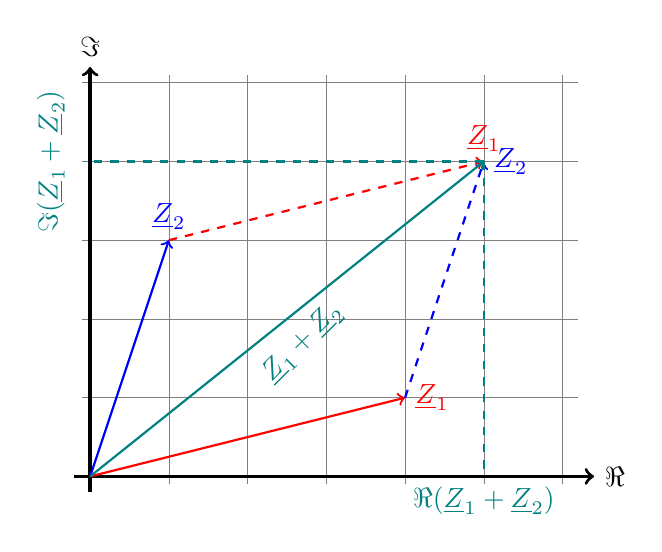
\begin{tikzpicture}
    \draw (0,0) coordinate (K);
    \draw[very thin,gray] (-0.1,-0.1) grid (6.2,5.1);
    \draw[->, very thick] (-0.2,0) -- (6.4,0) node[right] {$\Re$};
    \draw[->, very thick] (0,-0.2) -- (0,5.2) node[above] {$\Im$};
    \draw[->, thick, red] (0,0) -- (4,1) node[right] {$\underline{Z}_\mathrm{1}$};
    \draw[->, thick, blue] (0,0) -- (1,3) node[above] {$\underline{Z}_\mathrm{2}$};
    \pause

    \draw[->, dashed, thick, blue] (4,1) -- (5,4) node[right] {$\underline{Z}_\mathrm{2}$};
    \draw[->, dashed, thick, red] (1,3) -- (5,4) node[above] {$\underline{Z}_\mathrm{1}$};
    \pause

    \draw[->, thick, teal] (0,0) -- (5,4);
    \draw(2.7,1.7) node [teal, rotate=45] {$\underline{Z}_\mathrm{1}+\underline{Z}_\mathrm{2}$};
    \draw[dashed, thick, teal] (5,4) -- (0,4)
    (-0.5,4) node[rotate=90] {$\Im(\underline{Z}_\mathrm{1}+\underline{Z}_\mathrm{2}$)};
    \draw[dashed, thick, teal] (5,4) -- (5,0) node[below] {$\Re(\underline{Z}_\mathrm{1}+\underline{Z}_\mathrm{2}$)};
\end{tikzpicture}
    }{{\bf Addition von komplexen Zahlen.} Zeichnerische Lösung einer Addition von zwei komplexen Zahlen im Zeigerdiagramm. \label{BildKomplexRechnung}}

    \speech{KomplxGraphAdd}{1}{Gezeigt wird die Komplexe Ebene mit der Aufteilung in Realteil und Imaghinärteil.
    Außerdem werden die Zahlen Zett eins in rot und Zett zwei in blau dargestellt.
    Hier soll nun die Addition der beiden komplexen Zahlen grafisch gelöst werden.}
    \speech{KomplxGraphAdd}{2}{Dafür wird eine der Zahlen parallel an der anderen komplexen Zahl verschoben. 
    Dabei ist es nach dem Kommutativgesetz unerheblich, welche komplexe Zahl womit addiert wird.}
    \speech{KomplxGraphAdd}{3}{Nun können der Realteil und der Imaginärteil aus der Summe der beiden komplexen Zahlen abgelesen und notiert werden.}
\end{frame}


\begin{frame}
    \ftx{Zeigerdiagramme - Subtraktion}

    \s{
        Die zeichnerische Lösung der Subtraktion von komplexen Zahlen erfolgt vergleichbar mit der Addition. 
        Zu beachten ist dabei, dass wie in anderen Zahlensystemen bei der Subtraktion von zwei komplexen Zahlen
        das Kommutativgesetz nicht gilt. Wird von der komplexen Zahl $Z_\mathrm{2}$ $Z_\mathrm{1}$ subtrahiert, ändert sich die Richtung
        von $Z_\mathrm{1}$. Hier erfolgt dann wieder die Parallelverschiebung, allerdings lediglich von $Z_\mathrm{1}$. An dem sich ergebenen
        neuen Vektor können dann wieder der Realteil und der Imaginärteil abgelesenw erden. 
    }

    \b{
        Rechenoperationen im Zeigerdiagramm - Subtraktion:

        \begin{itemize}
            \item[1.] <1-> Zeigerumkehr bei Negation
            \item[2.] <2-> Zeiger $Z_\mathrm{1}$ verschieben: Fußpunkt von $Z_\mathrm{1}$ zur Spitze von $Z_\mathrm{2}$
            \item[3.] <3-> Realteil und Imaginärteil ablesen
        \end{itemize}
    }

    \fu{
        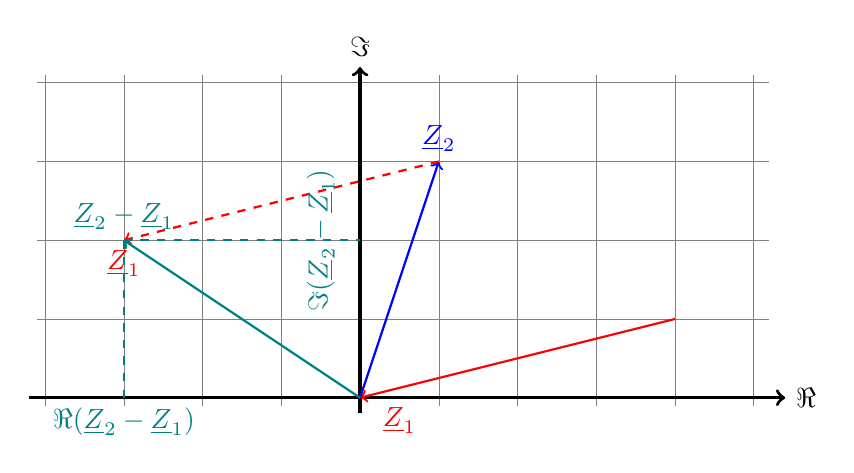
\begin{tikzpicture}
    \draw (0,0) coordinate (K);
    \draw[very thin,gray] (-4.1,-0.1) grid (5.2,4.1);
    \draw[->, very thick] (-4.2,0) -- (5.4,0) node[right] {$\Re$};
    \draw[->, very thick] (0,-0.2) -- (0,4.2) node[above] {$\Im$};
    \draw[->, thick, red] (4,1) -- (0,0);
    \draw(0.5,0) node [below,red] {$\underline{Z}_\mathrm{1}$};
    \draw[->, thick, blue] (0,0) -- (1,3) node[above] {$\underline{Z}_\mathrm{2}$};
    \pause

    \draw[->, dashed, thick, red] (1,3) -- (-3,2) node[left, below] {$\underline{Z}_\mathrm{1}$};
    \pause

    \draw[->, thick, teal] (0,0) -- (-3,2) node [teal, above] {$\underline{Z}_\mathrm{2}-\underline{Z}_\mathrm{1}$};
    \draw[dashed, thick, teal] (-3,2) -- (0,2)
    (-0.5,2) node[rotate=90] {$\Im(\underline{Z}_\mathrm{2}-\underline{Z}_\mathrm{1}$)};
    \draw[dashed, thick, teal] (-3,2) -- (-3,0) node[below] {$\Re(\underline{Z}_\mathrm{2}-\underline{Z}_\mathrm{1}$)};
\end{tikzpicture}
    }{{\bf Subtraktion von komplexen Zahlen.} Zeichnerische Lösung einer Subtraktion von zwei komplexen Zahlen im Zeigerdiagramm.}

    \speech{KomplxGraphSub}{1}{Ähnlich wie bei der Addition wird bei der Subtraktion von komplexen Zahlen vorgegangen.
    Wieder wird die komplexe Ebene mit dem Realteil und dem Imaginärteil dargestellt.
    Nun wird aber Zett eins von Zett zwei subtrahiert. 
    Hierfür wird die Richtung des Zeigers Zett eins umgekehrt. }
    \speech{KomplxGraphSub}{2}{Anschließend wird der Zeiger von Zett eins so verschoben,
    dass das Ende von Zett eins an der Spitze von Zett zwei anliegt.}
    \speech{KomplxGraphSub}{3}{Folgend werden wieder der Realteil und der Imaginärteil aus der Differenz der beiden komplexen Zahlen abgelesen und notiert.}
\end{frame}

  
\begin{frame}
    \ftx{Zeigerdiagramme - Multiplikation}

    \s{
        Die in der Abbildung \ref{BildMultiplikation} dargestellten komplexen Zahlen $\underline{Z}_\mathrm{1}$ und $\underline{Z}_\mathrm{2}$ werden zur 
        Multiplikation in Polar-Koordinaten abgebildet. Durch die zuvor beschriebenen Rechnenregeln der Multiplikation 
        für komplexe Zahlen können die Werte für die für das Ergebnis $\underline{Z}_\mathrm{3}$ bestimmt werden. Die Multiplikation
        aus den Zeigerlängen gibt die Länge des Produktes an. Die Summe aus den beiden komplexen Zahlen den Winkel der neuen
        komplexen Zahl an. 
    }

    \b{
        Rechenoperationen im Zeigerdiagramm - Multiplikation: (Zeichnung nicht maßstabsgetreu!)

        \begin{itemize}
            \item[1.] <2-> Winkel $\varphi_\mathrm{1}+\varphi_\mathrm{2}$ berechnen und einzeichnen
            \item[2.] <3-> Länge $Z_1 \cdot Z_\mathrm{2}$ berechnen und eintragen
            \item[3.] <4-> Realteil und Imaginärteil ablesen
        \end{itemize}
    }
    
    \fu{
        \begin{tikzpicture}
    \draw (0,0) coordinate (U);
    \draw (4,0) coordinate (0);
    \draw[very thin,gray] (-3.1,-0.1) grid (5.2,4.1);
    \draw[->, very thick] (-3.2,0) -- (5.4,0) node[right] {$\Re$};
    \draw[->, very thick] (0,-0.2) -- (0,4.2) node[above] {$\Im$};
    \draw[->, thick, red] (0,0) -- (4,1) coordinate (1);
    \draw(4,1) node [right,red] {$\underline{Z}_\mathrm{1}$};
    \draw[->, thick, blue] (0,0) -- (1,3) coordinate (2);
    \draw(1,3) node [above,blue] {$\underline{Z}_\mathrm{2}$};
    \draw pic[draw,red, very thick, angle radius = 3cm, ->] {angle = 0--U--1} (3.5,0.5) node[very thick, red]{$\varphi_\mathrm{1}$};
    \draw pic[draw,blue, very thick, angle radius = 2cm, ->] {angle = 0--U--2} (1.5,1.7) node[very thick, blue]{$\varphi_\mathrm{2}$};
    \pause

    \draw (-2,4) coordinate (3);
    \draw pic[draw, teal, very thick, angle radius = 1cm, ->] {angle = 0--U--3} (-1.2,0.5) node[very thick, teal]{$\varphi_\mathrm{1}+\varphi_\mathrm{2}$};
    \pause

    \draw[->, thick, teal] (0,0) -- (-2,4);
    \pause

    \draw[dashed, thick, teal] (-2,0) -- (-2,4) node[above] {$\underline{Z}_\mathrm{2} \cdot \underline{Z}_\mathrm{1}$};
    \draw[dashed, thick, teal] (0,4) -- (-2,4);
\end{tikzpicture}
    }{{\bf Multiplikation von komplexen Zahlen.} Zeichnerische Lösung einer Multiplikation von zwei komplexen Zahlen in Polar-Koordinaten im Zeigerdiagramm. \label{BildMultiplikation}}

    \speech{KomplxGraphMulti}{1}{Bei der grafischen Multiplikation ist ein wenig Rechnen notwendig.
    Hier werden die komplexen Zahln Zett eins und Zett zwei in der komplexen Ebene in ihrer Polarform dargestellt.}
    \speech{KomplxGraphMulti}{2}{Um das Produkt aus den beiden komplexen Zahlen zu bestimmen,
    wird im ersten Schritt die Summe aus den beiden Winkel der komplexen Zahlen gebildet und notiert.}
    \speech{KomplxGraphMulti}{3}{Im zweiten Schritt werden die beiden Beträgen der komplexen Zahlen miteinander multipliziert und eingetragen.}
    \speech{KomplxGraphMulti}{4}{Abschließend kann das Ergebniss nach der Berechnung auch grafisch veranschaulicht werden.}
\end{frame} 
\newpage
%Anwendung komplexe Zahlen in der Wechselstromtechnik

\newvideofile{Zeiger}{Zeigerdiagramme}

\begin{frame}
    \fta{Zeigerdiagramme in der Wechselstromtechnik}
    
    \s{
        In der Wechselstromtechnik finden die komplexen Zahlen unter Anderem als Zeiger Verwendung.  
        In linearen Netzwerken haben sinusförmige und monofrequente Quellengrößen nur sinusförmige und monofrequente 
        Spannungen und Ströme zur Folge. Im Stationären Zustand unterscheiden sich die Spannungen und Ströme nur in 
        ihrer Amplitude und der zugehörigen Phase. Alle Signale haben dabei eine identische Frequenz. Die Stationären
        und harmonischen Schwingungen können durch ihren Zeitverlauf im Liniendiagramm oder durch komplexe Zahlen durch
        Zeiger dargestellt werden. Die Beschreibung von Schwingungen durch komplexe Zahlen ermöglicht die Darstellung 
        durch ruhende Zeiger, wobei nur die relative Lage zueinander ausgedrückt wird. 
    }
    
    \begin{Lernziele}{Zeigerdiagramme}
        Die Studierenden
        \begin{itemize}
            \item verstehen die Kenngrößen von periodischen Wechselspannungen.
            \item können mit den komplexen Drehzeigern der Amplituden umgehen.
        \end{itemize}
    \end{Lernziele}
    
    \speech{ZeigerLrnz}{1}{Zeigerdiagramme dienen in der Wechselstromtechnik der vereinfachten Berechnung von sinusförmigen Wechselgrößen.
    In diesem Kapitel sollen die Kenngrößen von periodischen Wechselgrößen vermittelt 
    und die zugehörigen komplexen Drehzeiger erläutert werden.} 
\end{frame}

\begin{frame}
    \ftb{Periodische Wechselspannung}
    
    \s{
        In der Abbildung \ref{BildWechselspannungssignal} wird ein Wechselspannungssignal mit dem Scheitelwert (Amplitudenwert) $\hat{U}$
        dargestellt. Der Versatz des Wechselspannungssignals auf der Abszisse wird durch den Zeitpunkt $t_\mathrm{0}$
        ausgedrückt. Der Punkt in dem das Wechselspannungssignal die Ordinate kreuzt gibt den Wechselspannungswert 
        $U$ zum Zeitpunkt $t=0$ an. 
        
        Das Wechselspannungssignal ist periodisch in $T$. Eine Periode wird bei dem angegebenen Wechselspannungsignal
        durch einen kompletten Durchlauf einer positiven und negativen Halbwelle definiert. So wird ab $t_\mathrm{0}$ nach einer 
        Periode der Zeitpunkt $t_0+T$ und nach zwei Perioden der Zeitpunkt $t_\mathrm{0+2T}$ erreicht. 
        
        Mit der Übertragung der angegebenen Werte auf ein Kreisdiagramm lässt sich der Zusammenhang der Wechselspannung 
        mit der komplexen Darstellung erklären. Auf diese Weise kann die Wechselspannungsgröße $U(t=0)$ zum Zeitpunkt $0$ 
        durch die Länge und Ausrichtung des Zeigers beschrieben werden. Der Scheitelwert enspricht der Länge des Zeigers
        im Kreisdiagramm. Der Winkel $\varphi_\mathrm{u}$ beschreibt den Phasenwinkel zum Zeitpunkt $t=0$. 
    }
    
    \b{
        Anwendung von komplexen Zahlen in der Wechselstromtechnik
        
        \begin{itemize}
            \item <1-> Sinusförmige und harmonische Quellengrößen, Scheitelwert $\hat{U}$ und Phasenverschiebung $t_\mathrm{0}$
            \item <2-> Periodendauer $T$, Wiederholung von Perioden
            \item <3-> Stationärer Zustand $\rightarrow$ Spannungen und Ströme unterscheiden sich nur in Amplitude und Phase
            \item <4-> Schwingungen können durch Zeiger dargestellt werden
        \end{itemize}
    }
    
    \fu{
        %vergrößern auf Folienbreite
        \resizebox{0.95\textwidth}{!}{
            \begin{circuitikz}[domain=-1:8.5,samples=100]
    %Gitter
    \draw[very thin,color=gray] (-1.1,-2.1) grid (8.7,2.1);
    \draw[->] (-1.2,0) -- (8.9,0) node[right] {$t$};
    \draw[->] (0,-2.1) -- (0,2.2) node[above] {};
    \draw (0,-2.1) node[below] {$0\ ms$};
    \draw (2,-2.1) node[below] {$10\ ms$};
    \draw (4,-2.1) node[below] {$20\ ms$};
    \draw (6,-2.1) node[below] {$30\ ms$};
    \draw (8,-2.1) node[below] {$40\ ms$};
    \draw[color=voltage] (0,2.2) node[above] {$u(t)$};
    \draw[color=voltage, very thick] plot[id=Sinus6] function{1.5 * sin((pi/2) * x + (pi/4))} node[right] {};
    \draw(0,-2.1) -- (0,2.2) node[above] {};
    \draw[dashed](0,1.5) -- (1.5,1.5) node[above] {$\hat{U}$};
    \draw[dashed](0.2,1) -- (-0.2,1) node[above left] {$u(t=0)$};
    \draw (-0.5,0.2) -- (-0.5,-0.2) node[below] {$t_\mathrm{0}$};
    \pause

    %Periodendauer
    \draw (3.5,0.2) -- (3.5,-0.2) node[below right] {$t_\mathrm{0+T}$};
    \draw (7.5,0.2) -- (7.5,-0.2) node[below right] {$t_\mathrm{0+2T}$};
    \draw[dashed](3.5,0) -- (3.5,2);
    \draw[dashed](7.5,0) -- (7.5,2);
    \draw[<->] (3.5,2) -- (7.5,2);
    \draw (5.5,2) node[above] {T};
    \pause

    %Kreisdiagramm
    \draw (11.5,-2) -- (11.5,2);
    \draw (9.5,0) -- (13.5,0);
    \draw (11.5,0) circle (1.5);
    \draw[dashed](8.5,1.5) -- (11.5,1.5);
    \draw (9.5,1.5) node[above] {$\hat{U}$};
    \draw[dashed](7.8,1) -- (12.5,1);
    \draw (9,0.6) node {$u(t=0)$};
    \pause

    %Zeiger und Winkel
    \draw[->] (11.5,0) -- (12.55,1.05);
    \draw (13,0) coordinate (3);
    \draw (11.5,0) coordinate (4);
    \draw (13,1.5) coordinate (5);
    \draw pic[draw, very thick, angle radius = 0.75cm, ->] {angle = 3--4--5};
    \draw (12.5,0.5) node[very thick]{$\varphi_\mathrm{u}$};
    \draw (13.5,1) coordinate (6);
    \draw (11.5,0) coordinate (7);
    \draw (12.5,2) coordinate (8);
    \draw pic[draw, thick, angle radius = 1.7cm, ->] {angle = 6--7--8};
    \draw (12.8,1.7) node[very thick]{$\omega=\frac{2 \pi}{T}$};
    \def\StartAngle{0}
    \def\EndAngle{359}
    \def\Radius{1.5}
    \draw([shift=(\StartAngle : \Radius)]11.5,0)  arc[start angle=\StartAngle, end angle=\EndAngle, radius=\Radius];
    %\draw (9.3,0.9) node[right] {$\varphi_i=\frac{\pi}{2}$};									

    %ohne diesen Befehl macht das \pause in der Tikz Umgebung die Footline kaputt
    \onslide<1->
\end{circuitikz}
        }
    }{{\bf Periodische Wechselspannung über der Zeit mit zwei Perioden.} Anhand der Wechselspannung lassen sich z.B. der
        Amplitudenwert und die Periodedauer ermitteln.   \label{BildWechselspannungssignal}}

    \speech{ZeigerPerd}{1}{Folgend wird eine Sinusförmige und harmonische, also gleichförmige Wechselspannung dargstellt. 
    Der größtmögliche Ausschlag des Spannungssignals wird beim sogenannten Scheitelwert U Dach erreicht.
    Außerdem kann ein Stromsignal oder Spannungssignal eine Phasenverschiebung T null aufweisen.}
    \speech{ZeigerPerd}{2}{Die Periodendauer T gibt hierbei die Länge einer Periode an. Das Spannungssignal wird periodisch wiederholt.}
    \speech{ZeigerPerd}{3}{Neben dieser Darstellung einer Wechselgröße, kann in einem Stationären Zustand, also zu einem festgesetzten Zeitpunkt,
    quasi ein Momentwert einer Wechselspannung oder eines Wechselstroms beschrieben werden. 
    Die Beschreibung von sinusförmigen Wechselgrößen erfolgt hier mit dem Amplitudenwert und der Phase.}
    \speech{ZeigerPerd}{4}{So lässt sich die Schwingung der Wechselgrößen auch als Zeiger darstellen.
    Der Zeiger dreht sich hierbei um den Kreis mit der Kreisfrequenz.}
\end{frame}

\begin{frame}
    \ftx{Umrechnung der Kreisfrequenz}
    
    \s{
        Die Kreisfrequenz $\omega$ kann mithilfe der Periodendauer $T$ oder der Frequenz $f$ angegeben werden. Weiter wird die 
        Kreisfrequenz auch als Winkelgeschwindigkeit beschrieben. Über den 
        Zusammenhang zwischen der Periodendauer und der Frequenz können die Größen ineinander umgerechnet werden. 
        Die erläuterten Zusammenhänge werden in den Gleichungen \ref{GleichungKreisfrequenz} beschrieben.
    }
    
    \b{
        \begin{itemize}
            \item Kreisfrequenz $\omega$ beschrieben durch die Periodendauer $T$
            \item<2-> Umrechnung von Periodendauer und Frequenz $f$
            \item<3-> Kreisfrequenz $\omega$ beschrieben durch die Frequenz
        \end{itemize}
    }
    
    \begin{eq}
        \omega = \frac{2\pi}{T} 
        \onslide<2->{\text{\quad mit \quad} f=\frac{1}{T} }
        \onslide<3->{\text{\quad wird \quad} \omega = 2\pi f \label{GleichungKreisfrequenz}}
    \end{eq}

    \speech{ZeigerKreis}{1}{Die Kreisfrequenz Omega lässt sich wie angegeben aus der Periodendauer T errechnen.
    Der Ausdruck zwei Pi erfolgt aus dem Umlauf eines Kreises im Bogenmaß.}
    \speech{ZeigerKreis}{2}{Über die Periodendauer kann auch eine Verbindung zur Frequenz f hergeleitet werden.
    Die Frequenz einer Wechselspannung lässt sich aus dem Kehrwert der Periodendauer bestimmen.}
    \speech{ZeigerKreis}{3}{So kann die Kreisfrequenz auch über die frequenz errechnet werden.}
\end{frame}

\begin{frame}
    \ftx{Harmonische Wechselgrößen}
    
    \s{
        Angenommen der Durchlauf einer kompletten Periode bei einer Frequenz von $50 Hz$ dauert $20 ms$ (vgl. Abbildung \ref{BildZeiten}). 
        Übertragen auf das Gradmaß und das Radmaß ergeben sich so Winkelangaben für den Durchlauf einer Periode. Der 
        Winkel nach der kompletten Periode T entspricht dem Umlauf eines vollen Kreises. Der Umlauf eines vollen Kreises
        entspricht dazu 
        Die Phasenverschieben $t_\mathrm{0}$
        lässt sich auch in der Winkeldarstellung als Phasenwinkel $\varphi_\mathrm{N}$ beschreiben. 
    }
    
    \b{
        \begin{itemize}
            \item <1-> Eine Periodendauer entspricht in Winkelgrößen einem Kreisumlauf von $360°$ oder $2\pi$
            \item <2-> Die Phasenverschiebung $t_\mathrm{0}$ entspricht in der Winkeldarstellung dem Phasenwinkel $\varphi_\mathrm{N}$
        \end{itemize}
    }
    
    \fu{
        \begin{circuitikz}
    \draw[very thin,color=gray] (-1.1,-0.1) grid (8.7,0.3);
    \draw[->] (-1.2,0) -- (8.9,0) node[right] {t in ms};
    \draw (0,-0.1) node[below] {$0$};
    \draw (2,-0.1) node[below] {$5$};
    \draw (4,-0.1) node[below] {$10$};
    \draw (6,-0.1) node[below] {$15$};
    \draw (8,-0.1) node[below] {$20$};
    \draw[dashed,GETgreen](-1.2,-0.6) -- (10.3,-0.6);
    \draw[very thin,color=gray] (-1.1,-1.1) grid (8.7,-0.7);
    \draw[->] (-1.2,-1) -- (8.9,-1) node[right] {Grad};
    \draw (0,-1.1) node[below] {$0$};
    \draw (2,-1.1) node[below] {$90$};
    \draw (4,-1.1) node[below] {$180$};
    \draw (6,-1.1) node[below] {$270$};
    \draw (8,-1.1) node[below] {$360$};
    \draw[very thin,color=gray] (-1.1,-2.1) grid (8.7,-1.7);
    \draw[->] (-1.2,-2) -- (8.9,-2) node[right] {Rad};
    \draw (0,-2.1) node[below] {$0$};
    \draw (2,-2.1) node[below] {$\pi/2$};
    \draw (4,-2.1) node[below] {$\pi$};
    \draw (6,-2.1) node[below] {$3/2 \pi$};
    \draw (8,-2.1) node[below] {$2\pi$};
    \draw[dashed](-0.5,0.3) -- (-0.5,-2.2);
    \draw (-0.5,0.3) node[above] {$t_\mathrm{0}$};
    \draw (-0.5,-2.2) node[below] {$\varphi_\mathrm{N}$};
\end{circuitikz}
    }{{\bf Verschiedene Maßangaben.} Vegleich zwischen Gradmaß und Radmaß, der Umlauf eines Kreises entspricht $360^o$ oder
        $2\pi$. \label{BildZeiten}}

    \speech{ZeigerHarm}{1}{Wie bereits angemerkt entspricht die Periodendauer einem Kreisumlauf von zwei Pi oder Dreihundertsechzig grad.}
    \speech{ZeigerHarm}{2}{Die zuvor kennengelernte Phasenverschiebung T null, welche in der Zeiteinteilung und der Berechnung mit der Periodendauer zum Einsatz kommt,
    entspricht in der Winkeldarstellung Vieh N dem Phasenwinkel.}
\end{frame}



\begin{frame}
    \ftx{Wechselgrößen}
    
    \begin{Merksatz}{Wechselgrößen}
        Eine Wechselspannung erklärt einen regelmäßigen Polaritätswechsel mit dem {\bf Amplitudenwert $\hat{U}$} und der 
            {\bf Periodendauer $T$}.
    \end{Merksatz}
    
    \speech{ZeigerMrk1}{1}{Eine Wechselspannung erklärt einen regelmäßigen Polaritätswechsel mit dem Amplitudenwert U Dach und der Periodendauer Tee.}
\end{frame}




\begin{frame}
    \ftx{Zeitabhängige Wechselspannung}
    
    \s{
        Der zeitabhängige Spannungswert $u(t)$ einer Wechselspannung ist von mehreren Einflussgrößen abhängig.
        Dazu gehören der Scheitelwert und die Frequenz der Wechselspannung sowie der dazugehörige Phasenwinkel.
        Über das Verhältnis vom Zeitpunkt t zur Periodendauer lässt sich $u(t)$ bestimmen.
    }
    
    \b{
        \begin{itemize}
            \item $u(t)$ beschrieben durch die Kreisfrequenz $\omega$
            \item $u(t)$ zum Zeitpunkt $t$ bei einer Periodendauer von $T$
        \end{itemize}
    }
    
    \begin{eq}
        u(t) = \hat{U} \cdot \sin(\omega t + \varphi_\mathrm{N}) = \hat{U} \cdot \sin(2\pi f t + \varphi_\mathrm{N}) = \hat{U} \cdot \sin(2\pi \frac{t}{T} + \varphi_N)       \label{GleichungSpannung}
    \end{eq}

    \speech{ZeigerZeitab}{1}{Je nachdem zu welchen Zeitpunkt klein T hat der Drehzeiger eine andere Ausrichtung.
    Der zeitabhängige Spannungswerte U von T wird in der Abhängigkeit von der Kreisfrequenz Omega beschrieben.}
\end{frame}




\begin{frame}
    \ftb{Komplexer Drehzeiger der Amplitude}
    
    \s{
        Der komplexe Spannungswert sowie der komplexe Stromwert können als Zeiger dargestellt werden. 
        Hier wird auf die Darstellungsart der Polar-Koordinaten zurückgegriffen. 
    }
    
    \b{
        \begin{itemize}
            \item lineare Netzwerke $\rightarrow$ Sinusförmige und harmonische Quellengrößen
            \item Stationärer Zustand $\rightarrow$ Spannungen und Ströme unterscheiden sich nur in Amplitude und Phase
            \item Schwingungen können durch Zeiger dargestellt werden
            \item Ruhende Zeiger drücken die relative Lage von Schwingungen zueinander aus
        \end{itemize}
    }
    
    \fu{
        \begin{tikzpicture}
    \draw (0,0) coordinate (U);
    %\draw[very thin,color=gray] (-0.1,-0.1) grid (3.2,2.1);
    \draw[->] (-0.2,0) -- (3.4,0) node[right] {$\Re$};
    \draw[->] (0,-0.1) -- (0,2.2) node[above] {$\Im$};
    \draw (3,0.02) coordinate (R);
    \draw (3,2.02) coordinate (Z);
    \draw[->, very thick, voltage] (0,0.02) -- (3,2.02);
    \draw pic[draw, very thick, angle radius = 2cm, ->, voltage] {angle = R--U--Z};
    \draw(1.4,0.5) node [voltage] {$\varphi_\mathrm{U}$};
    \draw(1,1)node [voltage] {$\hat{U}$};

    \draw (6,0) coordinate (U);
    %\draw[very thin,color=gray] (5.9,-0.1) grid (9.2,2.1);
    \draw[->] (5.8,0) -- (9.4,0) node[right] {$\Re$};
    \draw[->] (6,-0.1) -- (6,2.2) node[above] {$\Im$};
    \draw (9,0.02) coordinate (R);
    \draw (9,2.02) coordinate (Z);
    \draw[->, very thick, red] (6,0.02) -- (9,2.02);
    \draw pic[draw, very thick, angle radius = 2cm, ->, red] {angle = R--U--Z};
    \draw(7.4,0.5) node [red] {$\varphi_\mathrm{I}$};
    \draw(7,1)node [red] {$\hat{I}$};
\end{tikzpicture}
    }{{\bf Spannungs- und Stromzeiger.} Ein Spannungszeiger mit dazugehörigen Phasenwinkel und äquivalent dazu ein Stromzeiger mit Phasenwinkel\label{BildSpannung}}

    \speech{ZeigerZsm}{1}{Zusammenfassend kann gesagt werden, dass für lienare Netzwerke Sinusförmige und harmonische Quellengrößen gelten.
    In stationären Zuständen unterscheiden sich Spannungen und Ströme lediglich in ihrer Amplitude und Phase.
    Die Schwingungen können durch Zeiger dargestellt werden. Die Zeiger beruhen auf der Darstellung der Polarkoordinaten.
    Mithilfe von ruhenden Zeigern kann die relative Lage von Schwingungen zueinander ausgedrückt werden.}
\end{frame}

\begin{frame}
    \ftx{Komplexer Drehzeiger der Amplitude}
    
    \s{
        Eine harmonische Wechselgröße kann als mit konstanter Winkelgeschwindigkeit $\omega$ rotierender Zeiger dargestellt
        werden. Die Zeitfunktion ist die Projektion des Zeigers auf die reelle Achse. Der rotierende Zeiger wird durch 
        eine zeitabhängige komplexe Zahl beschrieben. Wie bei den komplexen Zahlen erklärt, können der Imaginärteil 
        und der Realteil jeweils sparat bestimmt werden. Über die Winkelfunktionen kann der Realteil und der 
        Imaginärteil der komplexen Spannung berechnet werden. 
    }
    
    \b{
        Komplexer Drehzeiger einer elektrischen Spannung:
        \begin{itemize}
            \item<1-> Amplitudenwert der Spannung: $\hat{U}$
            \item<2-> Phasenwinkel der Spannung: $\varphi_\mathrm{U}$
            \item<3-> Komplexe Spannungszeiger: $\underline{U}=\hat{U} \cdot e^{j \varphi_\mathrm{U}}$
            \item<4-> Realanteil der Spannung
            \item<5-> Imaginäranteil der Spannung
        \end{itemize}
    }
    
    \fu{
        \begin{tikzpicture}
    \draw (0,0) coordinate (U);
    %\draw[very thin,color=gray] (-0.1,-0.1) grid (3.2,3.1);
    \draw[->] (-0.2,0) -- (3.4,0) node[right] {$\Re(U)$};
    \draw[->] (0,-0.1) -- (0,3.2) node[above] {$\Im(U)$};
    \draw (3,0) coordinate (R);
    \draw (3,3) coordinate (Z);
    \draw[->, voltage] (0,0) -- (2.5,2.5);
    \draw(1,2) node [voltage] {$\hat{U}$};
    \pause

    \draw pic[draw, angle radius = 1cm, ->, voltage] {angle = R--U--Z};
    \draw(1.7,0.5) node [voltage] {$\varphi_\mathrm{U}$};
    \pause

    \draw(3,2.5) node [right,voltage] {$\underline{U}=\hat{U} \cdot e^{j \varphi_\mathrm{U}}$};
    \pause

    \draw[dashed](2.5,2.5) -- (2.5,-0.2) node[below] {$\hat{U} \cdot \cos(\omega t + \varphi_\mathrm{u})$};
    \pause

    \draw[dashed](2.5,2.5) -- (-0.2,2.5) node[left] {$\hat{U} \cdot \sin(\omega t + \varphi_\mathrm{u})$};
\end{tikzpicture}
    }{{\bf Zeigerdarstellung einer komplexen Wechselspannung.} Wechselspannungszeiger mit der Aufteilung in Realteil und
        Imaginärteil.}

    \speech{ZeigerDreh}{1}{Folgend wird beispielhaft der komplexe Drehzeiger einer elektrischen Spannung näher erläutert.
    Es werden der Imaginärteil und der Realteil in der komplexen Ebene der Spannung dargestellt.
    Außerdem ist der Drehzeiger mit der Information U Dach, also dem Amplitudenwert, eingezeichnet.}
    \speech{ZeigerDreh}{2}{Für die Darstellung in Polarkoordinaten fehlt noch der Phasenwinkel Vieh U in Relation zur Abszisse.}
    \speech{ZeigerDreh}{3}{Der komplexe Drehzeiger für die Komplexe Spannung U kann somit vollständig beschrieben werden.}
    \speech{ZeigerDreh}{4}{Der Anteil des Realteiles an der komplexen Spannung lässt sich über die trigonometrische Funktion
    des Cosinus bestimmen.}
    \speech{ZeigerDreh}{5}{Vergleichbar lässt sich der Imaginärteil mithilfe der Sinusfunktion berechnen.}
\end{frame}


\begin{frame}
    \ftx{Komplexe Drehzeiger von Spannung und Strom}
    
    \begin{Merksatz}{Komplexe Drehzeiger von Spannung und Strom}
        Die Wechselgrößen Spannung und Strom werden als komplexe Drehzeiger dargestellt. Die Drehzeiger beschreiben dabei 
            {\bf Augenblickswerte $u(t)$}, welche sich mit konstanter {\bf Winkelgeschwindigkeit $\omega$} verändern. 
    \end{Merksatz}

    \speech{ZeigerMrk2}{1}{Die Wechselgrößen Spannung und Strom werden als komplexe Drehzeiger dargestellt.
    Die Drehzeiger beschreiben dabei Augenblickswerte wie U von T, 
    welche sich mit konstanter Winkelgeschwindigkeit Omega verändern.}
\end{frame}



\begin{frame}
    \ftx{Spannungszeiger und Stromzeiger von elektrischen Komponenten}
    
    \s{
        Die Beschreibung von periodischen Größen an elektrischen Komponenten erfolgt durch feste Spannungszeiger und Stromzeiger. 
        Das Verhalten der verschiedenen Komponenten ist dabei jeweils unterschiedlich. In der Abbildung \ref{BildBauteileZeiger}
        werden ein Widerstand, ein Kondensator als Kapazität und eine Spule als Induktivität mit ihren zugehörigen Spannungs- und 
        Stromzeigern dargestellt. Das genaue Verhalten der drei Komponenten wird im folgenden Kapitel näher betrachtet. 
    }
    
    \b{
        Spannungszeiger und Stromzeiger für verschiedene Komponenten: 
        \begin{itemize}
            \item <1-> Elektrischer Widerstand $\rightarrow$ Spannungszeiger und Stromzeiger in Phase
            \item <2-> Kapazität $\rightarrow$ Stromzeiger eilt dem Spannungszeiger vor
            \item <3-> Induktivität $\rightarrow$ Stromzeiger folgt dem Spannungszeiger
        \end{itemize}
    }
    
    \fu{
        \resizebox{\textwidth}{!}{
            \begin{tikzpicture}
    \draw (0,0) coordinate (U);
    %\draw[very thin,color=gray] (-0.1,-0.1) grid (3.2,2.1);
    \draw[->] (-0.2,0) -- (3.4,0) node[right] {$\Re$};
    \draw[->] (0,-2.2) -- (0,2.2) node[above] {$\Im$};
    \draw (3,0.02) coordinate (R);
    \draw (3,2.02) coordinate (Z);
    \draw[->, voltage] (0,0) -- (3,2);
    \draw pic[draw, angle radius = 2.5cm, ->, voltage] {angle = R--U--Z};
    \draw(2.7,1.3) node [voltage] {$\varphi_\mathrm{UR}$};
    \draw(3,2)node [voltage,above] {$\hat{U}_\mathrm{R}$};
    \draw[->, red] (0,0.1) -- (1.5,1.1);
    \draw pic[draw, angle radius = 1.5cm, ->, red] {angle = R--U--Z};
    \draw(2,0.7) node [red] {$\varphi_\mathrm{IR}$};
    \draw(1.5,1.5)node [red] {$\hat{I}_\mathrm{R}$};
    \draw(0.5,4) to [R=$R$, v, i, name=R] (3.5,4);
    \varrmore{R}{$\underline{U}_\mathrm{R}$};
    \iarrmore{R}{$\underline{I}_\mathrm{R}$};
    \pause

    \draw (6,0) coordinate (U);
    %\draw[very thin,color=gray] (5.9,-0.1) grid (9.2,2.1);
    \draw[->] (5.8,0) -- (9.4,0) node[right] {$\Re$};
    \draw[->] (6,-2.2) -- (6,2.2) node[above] {$\Im$};
    \draw (9,0.02) coordinate (R);
    \draw (9,2.02) coordinate (Z);
    \draw[->, voltage] (6,0.02) -- (9,2.02);
    \draw pic[draw, angle radius = 2.5cm, ->, voltage] {angle = R--U--Z};
    \draw(8.7,1.3) node [voltage] {$\varphi_\mathrm{UC}$};
    \draw(9,2)node [voltage,above] {$\hat{U}_\mathrm{C}$};
    \draw[->, red] (6,0) -- (5,1.5) coordinate (C);
    \draw pic[draw, angle radius = 1.5cm, ->, red] {angle = R--U--C};
    \draw(6.5,1.7) node [red] {$\varphi_\mathrm{IC}$};
    \draw(5,1.5)node [red,above] {$\hat{I}_\mathrm{C}$};
    \draw(6.5,4) to [C=$C$, v, i, name=C] (9.5,4);
    \varrmore{C}{$\underline{U}_\mathrm{C}$};
    \iarrmore{C}{$\underline{I}_\mathrm{C}$};
    \draw (5,1.5) coordinate (K);
    \draw pic[draw, angle radius = 1cm] {angle = Z--U--K};
    \draw (6.1,0.5)[very thick] node {$\cdot$};
    \pause

    \draw (12,0) coordinate (U);
    %\draw[very thin,color=gray] (11.9,-0.1) grid (15.2,2.1);
    \draw[->] (11.8,0) -- (15.4,0) node[right] {$\Re$};
    \draw[->] (12,-2.2) -- (12,2.2) node[above] {$\Im$};
    \draw (15,0.02) coordinate (R);
    \draw (15,2.02) coordinate (Z);
    \draw[->, voltage] (12,0.02) -- (15,2.02);
    \draw pic[draw, angle radius = 2.5cm, ->, voltage] {angle = R--U--Z};
    \draw(14.7,1.3) node [voltage] {$\varphi_\mathrm{UL}$};
    \draw(15,2)node [voltage,above] {$\hat{U}_\mathrm{L}$};
    \draw[->, red] (12,0) -- (13,-1.5) coordinate (L);
    \draw pic[draw, angle radius = 1.5cm, <-, red] {angle = L--U--R};
    \draw(12.3,-1) node [red] {$\varphi_\mathrm{IL}$};
    \draw(13.5,-1.5)node [red,above] {$\hat{I}_\mathrm{L}$};
    \draw(12.5,4) to [L=$L$, v, i, name=L] (15.5,4);
    \varrmore{L}{$\underline{U}_\mathrm{L}$};
    \iarrmore{L}{$\underline{I}_\mathrm{L}$};
    \draw (13,-1.5) coordinate (M);
    \draw pic[draw, angle radius = 1cm] {angle = M--U--Z};
    \draw (12.5,-0.1)[very thick] node {$\cdot$};
\end{tikzpicture}
        }
    }{{\bf Verschiedene Bauteile und die Wechselspannungszeiger.} Die Bauteile Widerstand, Kondensator und Spule mit zugehörigen Spannungs- und Stromzeigern. \label{BildBauteileZeiger}}

    \speech{ZeigerKomp}{1}{Folgend ein Überblick über die Spannungszeiger und die Stromzeiger von drei Komponenten eines elektrischen Netzwerkes verschafft.
    Angefangen mit dem elektrischen Widerstand. Die komplexe Spannung und der komplexe Strom zeigen mit einem identischen Phasenwinkel in dieselbe Richtung.
    Der Spannungszeiger und der Stromzeiger sind somit in Phase.}
    \speech{ZeigerKomp}{2}{Bei einer Kapazität, also einem Kondensator, sind der Spannungszeiger und der Stromzeiger nicht in Phase, zeigen dementsprechend in unterschiedliche Richtungen.
    Der Stromzeiger eilt dem Spannungszeiger an einer Kapazität vor.}
    \speech{ZeigerKomp}{3}{An einer Induktivität, wie einer Spule, sind die Zeiger ebenfalls nicht in Phase. 
    Hier folgt der Stromzeiger dem Spannungszeiger nach.
    Wie es zu dieser Phasenverschiebung an Kapazitäten und Induktivitäten kommt, wird im Themengebiet der komplexen Wechselstromrechnung behandelt.}
\end{frame}


\newpage
%Komplexe Wechselstromrechnung

\begin{frame}
    \fta{Komplexe Wechselstromrechnung}
    
    \s{
        In Gleichstromnetzwerken wird mit konstanten Spannungsquellen und Stromquellen gearbeitet. Im Gegensatz dazu kommen bei der 
        komplexen Wechselstromrechnung Quellen mit sinusförmigen Wechselgrößen zum Einsatz. Die elektrische Analyse von Komponenten 
        in einem Wechselspannungsnetzwerk erfolgt komplex. 
        Die komplexen Spannungen \underline{U} und Ströme \underline{I} erzeugen zeitabhängige Spannungswerte u(t) und Stromwerte 
        i(t). Die Gleichung \ref{GleichungURIKomplex} beschreibt den angegebenen Zusammenhang zwischen komplexen und zeitabhängigen
        Strom- und Spannungswerten für einen ohmschen Widerstand.
    }
    
    \b{
        Komplexe und zeitabhängige Strom- und Spannungsangaben der Wechselstromrechnung:
    }
    
    \begin{eq}
        \underline{U} = \underline{Z}_\mathrm{R} \cdot \underline{I} \quad \rightarrow \quad u(t) = R \cdot i(t)  \label{GleichungURIKomplex}
    \end{eq}
    
    \s{
        Abgesehen von der komplexität der Wechselstromrechnungen, gelten weiterhin die Regeln zur Berechnung elektrischer Netzwerke,
        wie Maschen- und Knotenregeln, das Verhalten von Reihen- und Paralellschaltungen und die Knotenpotentialanalyse sowie die 
        Maschenstromanalyse. Bei all diesen Beispielen ist darauf zu achten, mit den komplexen Wechselgrößen zu rechnen. Für die 
        Erläuterung von elektrische Netzwerken mit komplexen Wechselgrößen werden im Folgenden diese Tehmengebiete näher betrachtet:
    }
    
    \b{
        Für die Berechnung von elektrische Netzwerken mit Wechselgrößen werden im Folgenden diese Tehmengebiete näher betrachtet:
    }
    
    
    \begin{Lernziele}{Wechselstromrechnung}
        Die Studierenden
        \begin{itemize}
            \item kennen die komplexe Impedanz und die komplexe Attmitanz.
            \item verstehen das Verhalten eines Widerstandes, eines Kondensators und einer Spule an einer Wechselspannung.
            \item kennen Wechselquellen und die dazugehörigen Umwandlungsvorschriften.
        \end{itemize}
    \end{Lernziele}
    
\end{frame}

\begin{frame}
    \ftb{Impedanz und Attmitanz in der komplexen Ebene}
    
    \s{
        Durch eine Phasenverschiebung zwischen der Spannung und dem Strom kommt es zu einer Erzeugung eines Blindanteils der Impedanz. Der Blindanteil lässt sich jedoch 
        auf der reellen Achse nicht darstellen, weshalb die reelle Achse um eine imaginäre Achse erweitert wird, welche gemeinsam die 
        komplexe Ebene bilden. Die Abbildung \ref{BildKomplexeImpedanz} zeigt den Zeiger der komplexen Impedanz in der komplexen Ebene 
        mit Imaginäranteil und Realanteil. 
        
        \fu{
            \begin{tikzpicture}
    \draw (0,0) coordinate (U);
    \draw[very thin,color=gray] (-0.1,-0.1) grid (3.2,3.1);
    \draw[->] (-0.2,0) -- (3.4,0) node[right] {$\Re(\underline{Z})$};
    \draw[->] (0,-0.1) -- (0,3.2) node[above] {$\Im(\underline{Z})$};
    \draw (3,0) coordinate (R);
    \draw (3,3) coordinate (Z);
    \draw[->] (0,0) -- (2.5,2.5);
    \draw(1.25,1.75) node {$\hat{Z}$};
    \draw pic[draw, angle radius = 1cm, ->] {angle = R--U--Z};
    \draw(1.2,0.5) node {$\varphi_Z$};
    \draw(3,2.5) node [right] {$\underline{Z}=\hat{Z} \cdot e^{j \varphi_\mathrm{Z}}$};
    \pause

    \draw[dashed](2.5,2.5) -- (2.5,-0.2) node[below] {$R$};
    \pause

    \draw[dashed](2.5,2.5) -- (-0.2,2.5) node[left] {$j \cdot X$};
\end{tikzpicture}
        }{{\bf Zeiger der komplexen Impedanz.} Die Impedanz in der komplexen Ebene mit der Aufteilung in Realanteil R und Imaginäranteil X. \label{BildKomplexeImpedanz}}
        
    }
    
    \b{
        \begin{minipage}[t]{0.4\textwidth}
            \begin{itemize}
                \item<1-> Komplexer Zeiger der Impedanz
                \item<2-> Wirkanteil der Impedanz
                \item<3-> Blindanteil der Impedanz
                \item<4-> Wirkwiderstand und Blindwiderstand der Impedanz
            \end{itemize}
        \end{minipage}
        \begin{minipage}[t]{0.4\textwidth}
            \fu{
                \begin{tikzpicture}
                    \draw (0,0) coordinate (U);
                    \draw[very thin,color=gray] (-0.1,-0.1) grid (3.2,3.1);
                    \draw[->] (-0.2,0) -- (3.4,0) node[right] {$\Re(\underline{Z})$};
                    \draw[->] (0,-0.1) -- (0,3.2) node[above] {$\Im(\underline{Z})$};
                    \draw (3,0) coordinate (R);
                    \draw (3,3) coordinate (Z);
                    \draw[->] (0,0) -- (2.5,2.5);
                    \draw(1.25,1.75) node {$\hat{Z}$};
                    \draw pic[draw, angle radius = 1cm, ->] {angle = R--U--Z};
                    \draw(1.2,0.5) node {$\varphi_Z$};
                    \draw(3,2.5) node [right] {$\underline{Z}=\hat{Z} \cdot e^{j \varphi_\mathrm{Z}}$};
                    \pause
                    
                    \draw[dashed](2.5,2.5) -- (2.5,-0.2) node[below] {$R$};
                    \pause
                    
                    \draw[dashed](2.5,2.5) -- (-0.2,2.5) node[left] {$j \cdot X$};
                \end{tikzpicture}
            }{}
        \end{minipage}
    }
    
    \s{
        So besteht auch die komplexe Impedanz \underline{Z} nach Gleichung \ref{GleichungImpedanz} aus einem Realteil und aus einem Imaginärteil. Der
        Realteil besteht aus dem ohmschen Anteil, welcher den Wirkwiderstand einer Impedanz darstellt. Der Wirkwiderstand wird auch als 
        Resistanz R bezeichnet. Zweiter Bestandteil der Impedanz ist der Imaginärteil, welcher auch als Reaktanz X bezeichnet wird.
        Die Reaktanz eines elektrischen Netzwerkes setzt sich beisplielsweise aus den kapazitiven und induktiven Auswirkungen zusammen
        und wird mit der imaginären Einheit j versehen. Die Einheit der komplexen Impedanz ist wie in der Gleichstromtechnik Ohm $\Omega$. 
    }
    
    \only<4>{
        \begin{eq}
            Impedanz = Resistanz + j \cdot Reaktanz \quad \rightarrow \quad \underline{Z} = R + j \cdot X   \label{GleichungImpedanz}
        \end{eq}
        \begin{eq}
            [\underline{Z}] = 1\ Ohm = 1\ \Omega \nonumber
        \end{eq}
    }
    
\end{frame}




\begin{frame}
    \ftx{Impedanz und Attmitanz in der komplexen Ebene}
    
    \s{
        Wie in der Gleichstromtechnik existiert ein Leitwert des elektrischen Widerstandes in der komplexen Wechselstromtechnik.
        Dieser Kehrwert der komplexen Impedanz wird als Admittanz \underline{Y} bezeichnet (vlg. Gleichung \ref{GleichungImpedanzAttmitanz}). Die Einheit des komplexen Leitwertes bleibt 
        wie in der Gleichstromtechnik Siemens S. 
    }
    
    \b{
        Komplexer Leitwert als Kehrwert der komplexen Impedanz:
    }
    
    \begin{eq}
        R = \frac{1}{G} \quad \rightarrow \quad \underline{Z} = \frac{1}{\underline{Y}}   \label{GleichungImpedanzAttmitanz}
    \end{eq}
    
    \s{
        Auch die Admittanz lässt sich in einen Wirkleitwert und einen Blindleitwert differenzieren. 
        Der Wirkleitwert G der Admittanz wird als Konduktanz und der Blindleitwert B der Admittanz wird als Suszeptanz bezeichnet (vgl. Gleichung \ref{GleichungAdmittanz} ). 
    }
    
    \b{
        Wirkleitwert und Blindleitwert der Admittanz:
    }
    
    \begin{eq}
        Admittanz = Konduktanz + j \cdot Suszeptanz \quad \rightarrow \quad \underline{Y} = G + j \cdot B           \label{GleichungAdmittanz}
    \end{eq}
    
    \begin{eq}
        [\underline{Y}] = 1\ Siemens = 1\ S \nonumber
    \end{eq}
    
\end{frame}


\begin{frame}
    \ftx{Komplexe Impedanz und komplexe Admittanz}
    
    \begin{Merksatz}{Komplexe Impedanz und komplexe Admittanz}
        Der Gleichstromwiderstand wird bei einer {\bf Wechselspannung} zur {\bf komplexen Impedanz} \underline{Z}. Der 
        Kehrwert des Widerstandes, der Leitwert, wird bei einer Wechselspannung zur {\bf komplexen Admittanz} \underline{Y}.
    \end{Merksatz}
\end{frame}


\begin{frame}
    \ftb{Komplexer Widerstand}
    
    \s{
        Der komplexe Widerstand eines ohmschen Verbrauchers besteht aus dem Wirkannteil R und dem Blindanteil des des ohmschen 
        Widerstandes.
        Der ohmsche Widerstand R verkörpert die Eigenschaft leitfähiger Materialien elektrische Leistung in thermische Leistung 
        umzuwandeln. Der Blindanteil des Widerstands wandelt die Leistung der Wechselströme nicht in Wärme um. 
        Der Blindanteil des elektrischen Widerstands wird als $X_\mathrm{R}$ beziechnet. Da der ideale elektrische Widerstand allerdings rein
        ohmsch und damit rein Real wirkt, wird in der Regel oft einfach das Formelzeichen R verwendet. Die Gleichung \ref{GleichungWid1}
        erklärt diese Zusammenhänge. 
    }
    
    \b{
        \begin{itemize}
            \item Komplexer Widerstand an einem ohmschen Verbraucher
            \item Kein Blindanteil bei einem idealen ohmschen Widerstand
            \item Idealer komplexer Widerstand als reiner Wirkanteil
        \end{itemize}
    }
    
    \begin{eq}
        \underline{Z}_\mathrm{R} = R + j \cdot X_\mathrm{R} \quad \rightarrow \quad X_\mathrm{R-ideal} = j \cdot 0\ \Omega \quad \rightarrow \quad \underline{Z}_\mathrm{R} = R       \label{GleichungWid1}
    \end{eq}
    
    \s{
        An den zeitabhängigen Werten für die Spannung und den Strom ergeben sich die Zusammenhänge des idealen ohmschen Widerstandes 
        nach Gleichung \ref{GleichungWid2}. 
    }
    
    \begin{eq}
        \underline{U} = \underline{Z}_\mathrm{R} \cdot \underline{I} \quad \rightarrow \quad u(t) = R \cdot i(t)        \label{GleichungWid2}
    \end{eq}
    
\end{frame}

\begin{frame}
    \ftx{Komplexer Widerstand}
    
    \s{
        Ein idealer elektrischer Widerstand ist ein reiner Wirkwiderstand und weist keinerlei Blindwiderstandanteile auf. 
        Der reale elektrische Widerstand ist mit parasitären Effekten behaftet. Die Schaltbilder eines idealen und eines 
        realen elektrischen Widerstandes werden in der Abbildung \ref{BildRealerWiderstand} gegenübergestellt. Diese parasitären 
        Effekte wirken sich induktiv, verdeutlicht durch die Spule, und kapazitiv, verdeutlicht durch die Kapazität, auf die 
        Schaltung aus. Neben der Frequenzabhängikeit der parasitären Effekte, werden auch die Spannung und der Strom so aufgeteilt,
        dass nicht mehr die gesamte Leistung am Widerstand abfällt. die Impedanz des idealen elektrischenWiderstands ist nicht 
        frequenzabhängig.
    }
    
    \b{
        Elektrischer Widerstand in der Wechselstromrechnung
        \begin{itemize}
            \item<1-> Idealer Widerstand
            \item<2-> Realer Widerstand
            \item<3-> Keine Phasenverschiebung beim idealen Widerstand
        \end{itemize}
    }
    
    \fu{
        \begin{circuitikz}
    \draw (0,2) to [short, o-] (2,2)
    to [R=$R_\mathrm{ideal}$] (2,0)
    to [short,-o] (0,0);
    \pause

    \draw [->](4,1) -- (5,1);
    \draw (6,2) to [L=$L_\mathrm{paras.}$, o-*] (8,2)
    to [R=$R_\mathrm{real}$] (8,0)
    to [short,*-o] (6,0);
    \draw (8,2) to [short] (10,2)
    to [C=$C_\mathrm{paras.}$] (10,0)
    to [short] (8,0);

    %[R=$R_2$, i<, name=R2] (6,3);
    %\draw(0,0) to[V, V<, name=Uq1] (0,3);	
    %\varrmore{Uq1}{$U_{q1}$};
    %\iarrmore{R2}{$I_2$};}
\end{circuitikz}
    }{{\bf Gegenüberstellung eines idealen und eines realen elektrischen Widerstandes.} Der reale Widerstand weist im
        Gegensatz zum idealen Widerstand seriell induktive und parallel kapazitive Effekte auf. \label{BildRealerWiderstand}}
    
\end{frame}


\begin{frame}
    \ftx{Komplexer Widerstand}
    
    \s{
        Zwischen der Spannung und dem Strom existiert beim idealen elektrischen Widerstand keine Phasenverschiebung. In der 
        Abbildung \ref{BildPhasenWiderstand} werden die Sinuswellen für die Spannung und den Strom an einem idealen Widerstand 
        aufgetragen. Sie liegen ohne Phasenverschiebung übereinander, somit befinden sie sich in Phase. 
    }
    
    \b{
        Phasenverschiebung am idealen ohmschen Widerstand:
        \begin{itemize}
            \item<1-> Spannung $u_\mathrm{R}(t)$
            \item<2-> Strom $i_\mathrm{R}(t)$
            \item<3-> Spannung und Strom am idealen ohmschen Wiederstand ohne Phasenverschiebung
        \end{itemize}
    }
    
    \fu{
        \begin{tikzpicture}[scale=1.5]
    % Achsen
    \draw[->] (-0.5, 0) -- (4.2, 0) node[right] {Zeit $t$};
    \draw[->] (0, -1) -- (0, 1.2) node[right] {Amplitude};

    % Spannung (u)
    \draw[color=blue, very thick, smooth, domain=0:4] plot[id=Sinus31] function{sin(pi * x)} node[right] {};
    \node[blue] at (-0.5, 0.8) {$u_\mathrm{R}(t)$};
    \pause
    % Strom (i) - in Phase mit Spannung
    \draw[color=red, very thick, smooth, dashed, domain=0:4] plot[id=Sinus32] function{0.8 * sin(pi * x)} node[right] {};
    \node[red] at (-0.5, 0.5) {$i_\mathrm{R}(t)$};
    \pause
    \node at (0.5, -1.2) {$\Delta\varphi_\mathrm{R} = \varphi_\mathrm{U} - \varphi_\mathrm{I} = 0$};

\end{tikzpicture}
    }{{\bf Sinuschwingungen an einem Widerstand.} Wechselspannung (blau) und Wechselstrom (rot) an einem idealen Widerstand. Es resultiert an dem
        Widerstand keine Phasenverschiebung zwischen der Wechselspannung und dem Wechselstrom. \label{BildPhasenWiderstand}}
    
\end{frame}


\begin{frame}
    \ftx{Sinusschwingung an einem Widerstand}
    
    \begin{Merksatz}{Sinusschwingung an einem Widerstand}
        Der {\bf elektrische Widerstand} weist zwischen der Wechselspannung und dem zugehörigen Wechselstrom {\bf keine
                Phasenverschiebung} auf.     
    \end{Merksatz}
\end{frame}


\begin{frame}
    \ftb{Kapazität}
    
    \s{
        Der Kondesnator als Bauteil in der Elektrotechnik weist die Fähigkeit auf Energie zwischen den zwei Platten in 
        dem elektrischen Feld zu speichern. Die Größe eines Kondensators wird in der Kapazität C angegeben. Die Einheit 
        der Kapazität ist das Farad F. Die komplexe Impedanz eines Kondensators lässt sich nach Gleichung \ref{GleichungKap1}
        berechnen. Im Gegensatz zum idealen Widerstand wirkt der ideale Kondensator im Wechselstromkreis nicht lediglich als
        Wirkwiderstand. Der reale Kondensator wirkt sowohl durch einen Wirkwanteil, als auch durch einen Blindanteil. Die 
        Kreisfrequenz $\omega$ ist frequenzabhängig. So ergeben sich bei hohen Frequenzen niedrige Impedanzwerte für den 
        Kondensator. Andersherum ergeben sich hohe Impedanzwerte bei niedrigen Frequenzen. Der Blindanteil des Kondensators
        wirkt sich als kapazitive Reaktanz aus. 
        Es kann beim Kondensator auch mit der komplexen Admittanz gerechnet werden. Die komplexe Admittanz ergibt sich aus
        dem kehrwert der komplexen Impedanz des Kondensators. 
    }
    
    \b{
        Negativer Blindwiderstand $\leftrightarrow$ Darstellung im negativen Imaginärbereich
    }
    
    \begin{eq}
        \underline{Z}_\mathrm{C} = \frac{1}{j \omega C} \quad \rightarrow \quad \underline{Y}_\mathrm{C} = j \omega C          \label{GleichungKap1}
    \end{eq}
    
    \s{
        Der ideale Kondensator wirkt rein im Blindanteil, so wird nach Gleichung \ref{GleichungKap2} aus der komplexen Notation $Z_C$ der 
        Blindanteil des Kondensators $X_C$ mit zeitabhängiger Spannung und Strom. 
    }
    
    \b{
        Idealer Kondensator an Wechselspannung und Wechselstrom:  
    }
    
    \begin{eq}
        \underline{U} = \underline{Z}_\mathrm{C} \cdot \underline{I} \qquad \qquad u(t) = \underline{X}_\mathrm{C} \cdot i(t)     \label{GleichungKap2}
    \end{eq}
    
    \s{
        Es Wird davon ausgegangen, dass die Wechselspannung an einem Kondensator mit der Phasenverschiebung von 0° anliegt. 
        Mit dieser Feststellung kann die verursachte Phasenverschiebung des Stromes am Kondensator nach Gleichung \ref{GleichungKap3} festgelegt
        werden. Durch die Phasenverschiebung des Stromes gleicht der Verlauf einer Cosinusfunktion im Gegensatz zur Sinusfunktion
        der Spannung. Sollen sowohl die Spannung als auch der Strom durch die Sinusfunktion beschrieben werden, wird die 
        Phasenverschiebung $\Delta\varphi$ von $\pi/2$ ins Argument mit aufgenommen. 
    }
    
    \b{
        Pasenverschiebung des Stromes am idealen Kondensator: 
    }
    
    \begin{eq}
        u(t) = \hat{U} \cdot \sin(\omega t)      \qquad      i(t) = \hat{I} \cdot \cos(\omega t) = \hat{I} \cdot \sin(\omega t + \pi/2)        \label{GleichungKap3}
    \end{eq}
    
\end{frame}

\begin{frame}
    \ftx{Kapazität}
    
    \s{
        Bei Induktivitäten und Kapazitäten kommt es zu einer Phasenverschiebung zwischen der Wechselspannung und dem
        Wechselstrom. Beim Kondensator bedeutet dies, dass der Strom der Spannung um 90° (Gradmaß) voreilt. Der beschriebene 
        Sachverhalt der Phasenverschiebung wird in der Abbildung \ref{BildPhasenKondensator} verdeutlicht. Der in rot 
        dargestellte Strom an einem Kondensator erreicht den Maximalwert um $2\pi$ (Bogenmaß) früher als der blau gefärbte 
        Maximalwert der Spannung.  
    }
    
    \b{
        Phasenverschiebung am Kondensator:
        \begin{itemize}
            \item Spannung $u_\mathrm{C}(t)$
            \item<2-> Strom $i_\mathrm{C}(t)$
            \item<3-> Phasenverschiebung zwischen Strom und Spannung
            \item<4-> Phasenverschiebung $\Delta\varphi$
        \end{itemize}
    }
    
    \fu{
        \begin{tikzpicture}[scale=1.5]
    % Achsen
    \draw[->] (-0.5, 0) -- (4.2, 0) node[right] {Zeit $t$};
    \draw[->] (0, -1) -- (0, 1.2) node[right] {Amplitude};
    \draw (0.5,0.1) -- (0.5,-0.1);
    \draw (1,0.1) -- (1,-0.1) node[below] {$\pi$};
    \draw (1.5,0.1) -- (1.5,-0.1);
    \draw (2,0.1) -- (2,-0.1) node[below] {$2\pi$};

    % Spannung (u)
    \draw[color=blue, very thick, smooth, domain=0:4] plot[id=Sinus33] function{sin(pi * x)} node[right] {};
    \node[blue] at (-0.5, 0.8) {$u_\mathrm{C}(t)$};
    \node[blue] at (5, -0.5) {$\underline{U}=\hat{U} \cdot e^{j \varphi_\mathrm{U}}$};
    \pause
    % Strom (i) - in Phase mit Spannung
    \draw[color=red, very thick, smooth, dashed, domain=0:4] plot[id=Sinus34] function{0.8 * sin((pi * x)+(pi/2))} node[right] {};
    \node[red] at (-0.5, 0.5) {$i_\mathrm{C}(t)$};
    \node[red] at (5, 0.5) {$\underline{I}=\hat{I} \cdot e^{j \varphi_\mathrm{I}}$};
    \pause
    \draw[<->] (0.5, -0.2) -- (0, -0.2) node[below right] {$\pi/2$};
    \pause
    \node at (0.5, -1.2) {$\Delta\varphi_\mathrm{C} = \varphi_\mathrm{U} - \varphi_\mathrm{I} = -\pi/2$};
\end{tikzpicture}
    }{{\bf Phasenverschiebung zwischen Strom und Spannung an einem Kondensator.} Der Strom eilt der Spannung am Kondensator um 90° vor.
        \label{BildPhasenKondensator}}
    
\end{frame}


\begin{frame}
    \ftx{Sinusschwingung an einem Kondensator}
    
    \begin{Merksatz}{Sinusschwingung an einem Kondensator}
        An der idealen Kapazität eilt der Wechselstrom der Wechselspannung um 90° vor. 
    \end{Merksatz}
\end{frame}


\begin{frame}
    \ftx{Idealer und realer Kondensator}
    
    \s{
        In der Regel wird mit idealen Bauteilen und deren Eigenschaften gerechnet. Jedoch weist der reale Kondensator, wie auch 
        der zuvor beschriebene reale Widerstand, induktive und ohmsche parasitäre Effekte auf. Der ideale Kondensator wird in der 
        Abbildung \ref{BildRealerKondensator} dem realen Kondensator gegenübergestellt. Die Zu- und Ableitungen weisen induktive 
        ($L_\mathrm{paras.}$) und ohmsche ($R_\mathrm{paras.2}$) Anteile auf. Außerdem ist der Kondensator einer ständigen 
        Selbstentladung ausgesetzt. Diese Selbstentladung erfolgt symbolisch über den Paralellwiderstand $R_\mathrm{paras.1}$.
    }
    
    \b{
        Idealer und realer Kondensator:
        \begin{itemize}
            \item Idealer Kondensator
            \item<2-> Realer Kondensator mit parasitären Effekten
        \end{itemize}
    }
    
    \fu{
        \begin{circuitikz}
    \draw (0,2) to [short, o-] (2,2)
    to [C=$C_\mathrm{ideal}$] (2,0)
    to [short,-o] (0,0);
    \pause

    \draw [->](4,1) -- (5,1);
    \draw (6,2) to [L=$L_\mathrm{paras.}$, o-*] (8,2)
    to [C=$C_\mathrm{real}$] (8,0)
    to [R=$R_\mathrm{paras.2}$,*-o] (6,0);
    \draw (8,2) to [short] (10,2)
    to [R=$R_\mathrm{paras.1}$] (10,0)
    to [short] (8,0);
\end{circuitikz}
    }{{\bf Gegenüberstellung eines idealen und eines realen Kondensators.} Der reale Kondensator weist im
        Gegensatz zum idealen Widerstand seriell induktive und parallel kapazitive Effekte auf. \label{BildRealerKondensator}}
    
\end{frame}


\begin{frame}
    \ftb{Induktivität}
    
    \s{
        Die Spule stellt ebenso einen Energiespeicher dar, wie der Kondensator. Nur wird bei der Spule die Energie nicht in einem
        elektrischen Feld gespiechert, sondern in einem magnetischen Feld nach den Gegebenheiten der Induktionsgesetze. Die Größe
        einer Spule wird in der Induktivität L angegeben. Die Einheit der Induktivität ist Henry H. Die komplexe Impedanz einer Spule
        ergibt sich aus der Imaginären Einheit j, der Kreisfrequenz $\omega$ und der Induktivität L (vgl. Gleichung \ref{GleichungInd1}).
        die komplexe Admittanz wird durch den Kehrwert der Spulenimpedanz berechnet. Das führt zu Zusammenhängen, welche sich entgegen
        der Impedanzberechnungen bei Kapazitäten entwickeln. Bei hohen frequenzen werden die Impedanzen bei Spulen entsprechend ihrer 
        Induktivität ebenfalls groß und bei niedrigen Frequenzen entsprechend gering. 
    }
    
    \b{
        Positiver Blindwiderstand $\leftrightarrow$ Darstellung im positiven Imaginärbereich
    }
    
    \begin{eq}
        \underline{Z}_\mathrm{L} = j \omega L \quad \rightarrow \quad \underline{Y}_\mathrm{L} = \frac{1}{j \omega L}     \label{GleichungInd1}
    \end{eq}
    
    \s{
        Ebenso wie beim Kondensator wirkt die ideale Spule rein als Blindanteil der Impedanz. In der Gleichung \ref{GleichungInd2}
        wird auf der linken Seite die komplexe Notation der Spulenimpedanz $Z_L$ verwendet. Auf der rechten Seite wird die Zeitfunktion
        lediglich mit der Schreibweise des Blindanteils der Spule $X_L$ dargestellt.     
    }
    
    \b{
        Ideale Spule an Wechselspannung und Wechselstrom:  
    }
    
    \begin{eq}
        \underline{U} = \underline{Z}_\mathrm{L} \cdot \underline{I} \qquad  \qquad u(t) = \underline{X}_\mathrm{L} \cdot i(t)        \label{GleichungInd2}
    \end{eq}
    
    \s{
        Prinzipiell verhalten sich die Zeitfunktionen von Induktivitäten für die Spannung und den Strom vergleichbar, mit denen Zeitfunktionen
        von Kapazitäten. Lediglich die Phasenverschiebung des Stromes an Spulen ist der Phasenverschiebung der Kapazitäten entgegengesetzt. 
        Die Phasenverschiebung $\Delta\varphi$ zwischen der Spannung und dem Strom beträgt an einer Induktivität $\pi/2$. 
    }
    
    \b{
        Pasenverschiebung des Stromes an der idealen Spule: 
    }
    
    \begin{eq}
        u(t) = \hat{U} \cdot \cos(\omega t) = \hat{U} \cdot \sin(\omega t + \pi/2)    \qquad     i(t) = \hat{I} \cdot \sin(\omega t)      \label{GleichungInd3}
    \end{eq}
    
\end{frame}

\begin{frame}
    \ftx{Induktivität}
    
    \s{
        Äquivalent zu der Phasenverschiebung an einem Kondensator existiert an der Induktivität ebenfalls eine Phasenverschiebung.
        Jedoch ist diese Phasenverschiebung des Stromes an der Induktivität der Phasenverschiebung der Kapazität entgegengerichtet.
        Im konkreten Fall in der Abbildung \ref{BildPhasenSpule} wird gezeigt, dass der der Strom (rot) an einer Induktivität der 
        Spannung (blau) nacheilt. 
    }
    
    \b{
        Phasenverschiebung an der Spule:
        \begin{itemize}
            \item Spannung $u_\mathrm{L}(t)$
            \item<2-> Strom $i_\mathrm{L}(t)$
            \item<3-> Phasenverschiebung zwischen Strom und Spannung
            \item<4-> Phasenverschiebung $\Delta\varphi$
        \end{itemize}
    }
    
    \fu{
        \begin{tikzpicture}[scale=1.5]
    % Achsen
    \draw[->] (-0.5, 0) -- (4.2, 0) node[right] {Zeit $t$};
    \draw[->] (0, -1) -- (0, 1.2) node[right] {Amplitude};
    \draw (0.5,0.1) -- (0.5,-0.1);
    \draw (1,0.1) -- (1,-0.1) node[below] {$\pi$};
    \draw (1.5,0.1) -- (1.5,-0.1);
    \draw (2,0.1) -- (2,-0.1) node[below] {$2\pi$};

    % Spannung (u)
    \draw[color=blue, very thick, smooth, domain=0:4] plot[id=Sinus35] function{sin(pi * x)} node[right] {};
    \node[blue] at (-0.5, 0.8) {$u_\mathrm{L}(t)$};
    \node[blue] at (5, -0.5) {$\underline{U}=\hat{U} \cdot e^{j \varphi_\mathrm{U}}$};
    \pause
    % Strom (i) - in Phase mit Spannung
    \draw[color=red, very thick, smooth, dashed, domain=0:4] plot[id=Sinus36] function{0.8 * sin((pi * x)-(pi/2))} node[right] {};
    \node[red] at (-0.5, 0.5) {$i_\mathrm{L}(t)$};
    \node[red] at (5, 0.5) {$\underline{I}=\hat{I} \cdot e^{j \varphi_\mathrm{I}}$};
    \pause
    \draw[<->] (0.5, -0.2) -- (0, -0.2) node[below right] {$\pi/2$};
    \pause
    \node at (0.5, -1.2) {$\Delta\varphi_\mathrm{L} = \varphi_\mathrm{U} - \varphi_\mathrm{I} = +\pi/2$};
\end{tikzpicture}
    }{{\bf Phasenverschiebung zwischen Strom und Spannung an einer Spule.} Der Strom folgt der Spannung an der Spule um 90° nach.
        \label{BildPhasenSpule}}
    
\end{frame}



\begin{frame}
    \ftx{Sinusschwingung an einer Spule}
    
    \begin{Merksatz}{Sinusschwingung an einer Spule}
        Bei einer idealen Induktivität folgt der Wechselstrom der Wechselspannung um 90° nach.     
    \end{Merksatz}
\end{frame}


\begin{frame}
    \ftx{Ideale und reale Spule}
    
    \s{
        Wie auch der ohmsche Widerstand und der Kondensator weist die reale Spule parasitäre Effekte auf. Über den Spulendraht 
        wirkt ein ohmscher Anteil ($R_\mathrm{paras.}$) auf die komplexe Impedanz der Spule ein. Zusätzlich erzeugt die Wicklung 
        der Spule kapazitive Effekte ($C_\mathrm{paras.}$). In der Abbildung \ref{BildRealeSpule} wird das Ersatzschaltbild einer 
        idealen Spule und einer realen Spule dargestellt. 
    }
    
    \b{
        Ideale und reale Spule:
        \begin{itemize}
            \item Ideale Spule
            \item<2-> Reale Spule mit parasitären Effekten
        \end{itemize}
    }
    
    \fu{
        \begin{circuitikz}
    \draw (0,2) to [short, o-] (2,2)
    to [L=$L_\mathrm{ideal}$] (2,0)
    to [short,-o] (0,0);
    \pause

    \draw [->](4,1) -- (5,1);
    \draw (6,2) to [R=$R_\mathrm{paras.}$, o-*] (8,2)
    to [L=$L_\mathrm{real}$] (8,0)
    to [short,*-o] (6,0);
    \draw (8,2) to [short] (10,2)
    to [C=$C_\mathrm{paras.}$] (10,0)
    to [short] (8,0);
\end{circuitikz}
    }{{\bf Gegenüberstellung einer idealen und einer realen Spule.} Die reale Spule weist serielle ohmsche und parallele
        kapazitive parasitäre Effekte auf. \label{BildRealeSpule}}
    
\end{frame}


\begin{frame}
    \ftb{Quellen von Wechselgrößen}
    
    \s{
        Wie bei Quellen von Gleichströmen und Gleichspannungen existieren Wechselquellen mit vergleichbaren Merkmalen. Bei der
        idealen Wechselspannungsquelle ist die Spannung eingeprägt. Die Wechselspannung ändert sich nicht mit der Abhängigkeit 
        des Stromes, welcher durch sie hindurchfließt. Die ideale Wechselstromquelle stellt einen eingesprägten Strom zur 
        Verfügung. Dieser wird nicht durch die angeschlossene Last beeinflusst. Die Schaltungssymbole einer idealen 
        Wechselspannungsquelle und einer idealen Wechselstromquelle werden in der Abbildung \ref{BildIdealeQuellen} dargestellt. 
    }
    
    \b{
        Quellen von Wechselgrößen:
        \begin{itemize}
            \item Ideale Wechselspannungsquelle
            \item<2-> Ideale Wechselstromquelle
        \end{itemize}
    }
    
    \fu{
        \begin{circuitikz}
    \draw (0,0) to[vsourcesin] (0,2)
    to[short,-o] (2,2)
    (0,0) to[short,-o] (2,0);
    \draw[-latex, thick, draw=voltage] (2,1.8) to node[right, color=voltage] {$\underline{U}$} (2,0.2);
    \pause

    %\draw [->](4,1) -- (5,1); 

    \draw (6,0) to[vsourcesin, i^>, name=I] (6,2)
    to[short,-o] (8,2)
    (6,0) to[short,-o] (8,0);
    \iarrmore{I}{$\underline{I}$};
\end{circuitikz}
    }{{\bf Quellen von Wechselgrößen.} Ideale Wechselspannungsquelle und ideale Wechselstromquelle. \label{BildIdealeQuellen}}
\end{frame}


\begin{frame}
    \ftx{Reale Wechselspannungsquelle}
    
    \s{
        Bei den beiden vorgestellten Wechselquellen werden ideale Quellen abgebildet. Reale Wechselquellen weisen wie auch die 
        Quellen von Gleichspannungen und Gleichströmen Innenwiderstände auf. Diese Innenwiderstände prägen sich bei Quellen von 
        Wechselgrößen als komplexe Impedanzen aus. Die reale Wechselspannungsquelle hat also eine komplexe Innenimpedanz 
        $\underline{Z}_\mathrm{i}$, welche mit einer idealen Wechselspannungsquelle in Serie geschaltet ist. Bei realen 
        Wechselspannungsquellen ist die Ausgangsspannung $\underline{U}$ von der angeschlossenen Last abhängig. Die Gegenüberstellung
        einer idealen und einer realen Wechselspannungsquelle ist in der Abbildung \ref{BildIdealSpannung} dargestellt. 
    }
    
    \b{
        Wechselspannungsquelle:
        \begin{itemize}
            \item Ideale Wechselspannungsquelle
            \item<2-> Reale Wechselspannungsquelle mit Innenimpedanz $\underline{Z}_\mathrm{i}$
        \end{itemize}
    }
    
    \fu{
        \begin{circuitikz}
    \draw (0,0) to[vsourcesin] (0,2)
    to[short,-o] (2,2)
    (0,0) to[short,-o] (2,0);
    \draw[-latex, thick, draw=voltage] (2,1.8) to node[right, color=voltage] {$\underline{U}$} (2,0.2);
    \pause

    \draw [->](3,1) -- (4,1);

    \draw (6,0) to[vsourcesin, v^<, name=U] (6,2)
    to[R=$\underline{Z}_\mathrm{i}$, i^>, v, name=R, -o] (8,2)
    (6,0) to[short,-o] (8,0);
    \draw[-latex, thick, draw=voltage] (8,1.8) to node[right, color=voltage] {$\underline{U}$} (8,0.2);
    \varrmore{U}{$\underline{U}_\mathrm{0}$};
    \varrmore{R}{$\underline{U}_\mathrm{i}$};
    \iarrmore{R}{$\underline{I}$};
\end{circuitikz}
    }{{\bf Gegenüberstellung einer idealen und einer realen Wechselspannungsquelle.} Die reale Wechselspannungsquelle weist eine
        Serienimpedanz $\underline{Z}_\mathrm{i}$ auf. \label{BildIdealSpannung}}
    
    \s{
        Die Ausgangsspannung einer realen Wechselspannungsquelle lässt sich nach Gleichung \ref{GleichungQuel1} bestimmen. 
        Hier liegt die Wechselspannung der Wechselspannungsquelle nicht direkt an den Klemmen an. Sie wird durch die Spannung
        über die Innenimpedanz $Z_\mathrm{i}$ reduziert. 
    }
    
    \only<3>{
        \b{
            Ausgangsspannung einer realen Wechselspannungsquelle:
        }
        
        \begin{eq}
            \underline{U} = \underline{U}_\mathrm{0} - \underline{Z}_\mathrm{i} \cdot \underline{I}     \label{GleichungQuel1}
        \end{eq}
    }
\end{frame}

\begin{frame}
    \ftx{Charakteristik von realen Wechselspannungsquellen}
    
    \s{
        Reale Wechselspannungsquellen weisen gewisse Charakteristika ohne Last beim Leerlauf und bei einem Kurzschluss auf.
        Beim Leerlauf liegt zwischen den Klemmen eine unendlich große Impedanz. Es wird kein geschlossener Stromkreis gebildet 
        und es stellt sich kein Stromfluss ein (Gleichung \ref{GleichungQuel2}). Die gesamte Spannung der Wechselspannungsquelle 
        liegt an den offenen Klemmen an, siehe Gleichung \ref{GleichungQuel3}.
    }
    
    \b{
        Leerlauf:
    }
    
    \begin{eq}
        \underline{I} = 0 \qquad \rightarrow \qquad \underline{U}_\mathrm{i} = \underline{I} \cdot \underline{Z}_\mathrm{i} = 0 \label{GleichungQuel2}
    \end{eq}
    \begin{eq}
        \underline{U}_\mathrm{0} - \underline{U}_\mathrm{i} - \underline{U} = 0 \qquad \rightarrow \qquad \underline{U} = \underline{U}_\mathrm{0} \label{GleichungQuel3}
    \end{eq}
    
    \s{
        Beim Kurzschluss geht die Impedanz zwischen den Klemmen gegen null und es fällt dort keine Spannung ab. So stellt sich ein 
        größter möglicher Kurzschlussstrom ein, welcher lediglich durch die Innenimpedanz begrenzt wird (Gleichung \ref{GleichungQuel4}).
        Die Spannungs der Wechselspannungsquelle wirkt so in Gänze über die Innenimpedanz (Gleichung \ref{GleichungQuel5}). Der 
        Kurzschlussstrom lässt sich nach Gleichung \ref{GleichungQuel6} aus dem Verhältnis aus der Spannung über die Innenimpedanz 
        $\underline{U}_\mathrm{i}$ und der Innenimpedanz $\underline{Z}_\mathrm{i}$ bestimmen.
    }
    
    \b{
        Kurzschluss:
    }
    
    \begin{eq}
        \underline{U} = 0 \qquad \rightarrow \qquad \underline{I} = \underline{I}_\mathrm{k} \label{GleichungQuel4}
    \end{eq}
    \begin{eq}
        \underline{U}_\mathrm{0} - \underline{U}_\mathrm{i} - \underline{U} = 0 \qquad \rightarrow \qquad \underline{U}_\mathrm{i} = \underline{U}_\mathrm{0} \label{GleichungQuel5}
    \end{eq}
    \begin{eq}
        \underline{I}_\mathrm{k} = \frac{\underline{U}_\mathrm{i}}{\underline{Z}_\mathrm{i}} \label{GleichungQuel6}
    \end{eq}
    
\end{frame}


\begin{frame}
    \ftx{Beispielaufgabe}
    \begin{bsp}{Reale Spannungsquelle}{Reale Spannungsquelle:}
        
        \begin{enumerate}
            \only<1>{\item[]	
            
                  Eine Reale Spannungsquelle (230\ V, 50\ Hz) verfügt nach der unten stehenden Abbildung über eine Innenimpedanz $\underline{Z}_\mathrm{i}$, welche sich aus 
                  einer Spule $L=20\ mH$ und einem ohmschen Widerstand $R=10\ m\Omega$ zusammensetzt. 
                  
                  \fu{
                      \resizebox{0.5\textwidth}{!}{
                          \begin{circuitikz}
    \draw (0,0) to[vsourcesin, v^<, name=U] (0,2)
    to[L=$L$] (2,2)
    to[R=$R$, i^>, name=R, -o] (4,2)
    (0,0) to[short,-o] (4,0);
    \draw[-latex, thick, draw=voltage] (4,1.8) to node[right, color=voltage] {$\underline{U}$} (4,0.2);
    \varrmore{U}{$\underline{U}_\mathrm{0}$};
    \iarrmore{R}{$\underline{I}$};
\end{circuitikz}
                      }
                  }{{\bf Beispiel.} Wechselspannungsquelle mit einer Innenimpedanz aus einer Spule und einem Widerstand. \label{BildBeispielQuelle}}
                  
                  Bestimmen Sie die {\bf Leerlaufspannung} und den {\bf Kurzschlussstrom} der Wechselspannungsquelle.
                  }
                  
                  \only<2>{
            \item[] 
                  \onslide<2>{
                  \begin{eqa}
                      \underline{U}_\mathrm{0} &= 230\ V \cdot e^{\mathrm{j}0^o}          \nonumber    \\
                      \underline{Z}_\mathrm{i} &= R + j X_L       \nonumber    \\
                      \underline{Z}_\mathrm{i} &= 0,01\ \Omega + j \cdot 2\pi \cdot 50\ Hz \cdot 20\ mH      \nonumber    \\
                      \underline{Z}_\mathrm{i} &= 0,01\ \Omega + j 6,28\ \Omega       \nonumber
                  \end{eqa}
                  
                  {\bf Leerlaufspannung}:
                  \begin{eqa}
                      \underline{U} &= \underline{U}_\mathrm{0}        \nonumber    \\
                      \underline{U} &= 230\ V \cdot e^{\mathrm{j}0^o}         \nonumber
                  \end{eqa}
                  
                  {\bf Kurzschlussstrom}:
                  \begin{eqa}
                      \underline{I}_\mathrm{k} &= \frac{\underline{U}_\mathrm{0}}{\underline{Z}_\mathrm{i}}           \nonumber        \\
                      \underline{I}_\mathrm{k} &= \frac{230\ V \cdot e^{\mathrm{j}0^o}}{0,01\ \Omega + j 6,28\ \Omega}           \nonumber        \\
                      \underline{I}_\mathrm{k} &= (0,058 - j36,6)\ A = 36,6\ A \cdot e^{-\mathrm{j}89,9^o}    \nonumber
                  \end{eqa}
                  }
                  }    
        \end{enumerate}
    \end{bsp}
\end{frame}


\begin{frame}
    \ftx{Reale Wechselstromquelle}
    
    \s{
        Die reale Wechselstromquelle in der Abbildung \ref{BildIdealStrom} verfügt wie die Wechselspannungsquelle über 
        eine Innenimpedanz $\underline{Z}_\mathrm{i}$, wobei diese Innenimpedanz nicht wie bei der Wechselspannungsquelle 
        in serie geschlatet ist, sondern parallel zu einer idealen Wechselstromquelle liegt. Der sich ergebende Ausgangsstrom 
        $\underline{I}$ der Quelle ist von der angeschlossenen Last, bzw. von der Ausgangsspannung $\underline{U}$ abhängig. 
    }
    
    \b{
        Wechselstromquelle:
        \begin{itemize}
            \item<1-> Ideale Wechselstromquelle
            \item<2-> Reale Wechselstromquelle mit Innenimpedanz $\underline{Z}_\mathrm{i}$
        \end{itemize}
    }
    
    \fu{
        \begin{circuitikz}
    \draw (0,0) to[isourcesin, i, name=I1] (0,2)
    to[short,-o] (2,2)
    (0,0) to[short,-o] (2,0);
    \draw[-latex, thick, draw=voltage] (2,1.8) to node[right, color=voltage] {$\underline{U}$} (2,0.2);
    \pause

    \draw [->](3,1) -- (4,1);

    \draw (6,0) to[isourcesin, i, name=I2] (6,2)
    to [short] (8,2)
    to [short, i, name=S, -o] (10,2)
    (8,2) to [R=$\underline{Z}_\mathrm{i}$, i>^, name=R, *-*] (8,0)
    (6,0) to [short,-o] (10,0);
    \draw[-latex, thick, draw=voltage] (10,1.8) to node[right, color=voltage] {$\underline{U}$} (10,0.2);
    \iarrmore{I1}{$\underline{I}_\mathrm{0}$};
    \iarrmore{I2}{$\underline{I}_\mathrm{0}$};
    \iarrmore{R}{$\underline{I}_\mathrm{i}$};
    \iarrmore{S}{$\underline{I}$};
\end{circuitikz}
    }{{\bf Quellen von Wechselgrößen.} Ideale Wechselstromquelle und ideale Wechselstromquelle. \label{BildIdealStrom}}
    
    \s{
        Der Wechselstrom der idealen Wechselstromquelle wird durch einen Anteil durch die Innenimpedanz reduziert. Der 
        Ausgangsstrom der realen Wechselstromquelle lässt sich über die Gleichung \ref{GleichungQuel7} bestimmen. Hier 
        wird ausgehend vom Quellstrom $\underline{I}_\mathrm{0}$ der ausgangsspannungsabhängige ($\underline{U}$) 
        Wechselstromanteil  $\underline{I}_\mathrm{i}$ durch die Innenimpedanz $\underline{Z}_\mathrm{i}$ abgezogen.
    }
    
    \only<3>{
        \b{
            Ausgangswechselstrom einer realen Wechselstromquelle:
        }
        
        \begin{eq}
            \underline{I} = \underline{I}_\mathrm{0} - \underline{I}_\mathrm{i} = \underline{I}_\mathrm{0} - \frac{\underline{U}}{\underline{Z}_\mathrm{i}}     \label{GleichungQuel7}
        \end{eq}
    }
\end{frame}


\begin{frame}
    \ftx{Äquivalenz von Wechselquellen}
    
    \s{
        {\bf Wechselquellenumwandlung} \\
        
        
        Wechselstrom- und Wechselspannungsquellen können ineinander umgewandelt werden, wenn beide Wechselquellen den identischen
        Kurzschlussstrom und die gleiche Leerlaufspannung aufweisen. 
    }
    
    \b{
        Umwandlung von Wechselstromquellen und Wechselspannungsquellen:
    }
    
    \fu{
        \begin{circuitikz}
    \draw (0,0) to[vsourcesin, v^<, i^, name=U] (0,2)
    to[R=$\underline{Z}_\mathrm{i}$, i^>, v, name=R1, -o] (2,2)
    (0,0) to[short,-o] (2,0);
    \draw[-latex, thick, draw=voltage] (2,1.8) to node[right, color=voltage] {$\underline{U}$} (2,0.2);

    \draw [<->](3.5,1) -- (4.5,1);

    \draw (6,0) to[isourcesin, i, name=I2] (6,2)
    to [short] (8,2)
    to [short, i, name=S, -o] (10,2)
    (8,2) to [R=$\underline{Z}_\mathrm{i}$, i>^, name=R2, *-*] (8,0)
    (6,0) to [short,-o] (10,0);
    \draw[-latex, thick, draw=voltage] (10,1.8) to node[right, color=voltage] {$\underline{U}$} (10,0.2);
    \iarrmore{I2}{$\underline{I}_\mathrm{0}$};
    \iarrmore{R2}{$\underline{I}_\mathrm{i}$};
    \iarrmore{S}{$\underline{I}$};

    \varrmore{U}{$\underline{U}_\mathrm{0}$};
    \iarrmore{U}{$\underline{I}_\mathrm{0}$};
    \varrmore{R1}{$\underline{U}_\mathrm{i}$};
    \iarrmore{R1}{$\underline{I}$};
\end{circuitikz}
    }{{\bf Gegenüberstellung einer realen Wechselspannungsquelle und einer realen Wechselstromquelle.} Die reale Wechselspannungsquelle
        und die reale Wechselstromquelle sind ineinander umwandelbar. \label{BildQuelleUmwandlung}}
    
    \s{
        Beide Wechselquellen sind äquivalent, wenn nach Gleichung \ref{GleichungQuel8} und Gleichung \ref{GleichungQuel9} das ohmsche 
        Gesetz mit identischen Innenimpedanzen für die Wechselspannungsquelle und die Wechselstromquelle gilt. 
    }
    
    \b{
        Äquivalente Wechselquellen, bei identischen Innenimpedanzen:
    }
    
    \begin{eq}
        \underline{U}_\mathrm{0} = \underline{Z}_\mathrm{0} \cdot \underline{I}_\mathrm{0}      \label{GleichungQuel8}
    \end{eq}
    \begin{eq}
        \underline{Z}_\mathrm{i} = \underline{Z}_\mathrm{0}      \label{GleichungQuel9}
    \end{eq}
    
    \s{
        Hierbei soll der Kurzschlussstrom $\underline{I}_\mathrm{K}$ gleich dem Quellstrom $\underline{I}_\mathrm{0}$ der 
        Wechselstromquelle sein, welcher identisch zu dem Ausgangsstrom $\underline{I}$ ist. Die Ausgangswechselspannung
        $\underline{U}$ der Wechselquellen enspricht der Leerlaufspannung $\underline{U}_\mathrm{L}$.
    }
    
    \b{
        Quellstrom der Stromquelle gleich dem Kurzschlussstrom. \\
        Quellspannung der Spannungsquelle gleich der Leerlaufspannung.
    }
    
    \begin{eq}
        \underline{I} = \underline{I}_\mathrm{k} = \underline{I}_\mathrm{0} \qquad \text{und} \qquad \underline{U} = \underline{U}_\mathrm{L} = \underline{U}_\mathrm{0}     \label{GleichungQuel10}
    \end{eq}
    
\end{frame}



\begin{frame}
    \ftx{Beispielaufgabe}
    \begin{bsp}{Wechselquellenumwandlung}{Wechselquellenumwandlung:}
        
        \begin{enumerate}
            \only<1>{\item[]
                  Gegeben ist eine reale Wechselspannungsquelle mit $\underline{U}_\mathrm{0} = 20\ kV \cdot \mathrm{e}^{\mathrm{j}30^o}$ und 
                  $\underline{Z}_\mathrm{0} = (0,01 + j \cdot 2)\ \Omega$. Wandeln Sie die Wechselspannungsquelle in eine äquivalente 
                  Wechselstromquelle um, berechnen Sie hierzu den Kurzschlussstrom.\\
                  }
                  \only<2>{
            \item[] 
                  \onslide<2>{
                      {\bf Kurzschlussstrom:}
                      
                      
                      \begin{eq}
                          \underline{I}_\mathrm{0} = \frac{\underline{U}_\mathrm{0}}{\underline{Z}_\mathrm{0}}
                          = \frac{20\ kV \cdot \mathrm{e}^{\mathrm{j}30^o}}{(0,01 + j \cdot 2)\ \Omega}
                          = (5,04 + j \cdot 8,64)\ kA     \nonumber
                      \end{eq}
                  }
                  }
        \end{enumerate}
        
    \end{bsp}
\end{frame}


\begin{frame}
    \ftb{Komplexer Spannungsteiler und komplexer Stromteiler}
    
    \s{
        Wie bei der Betrachtung von Gleichstromnetzwerken gelten die Grundgesetze zur Analyse von Wechselstromnetzen.
        Die Knotenregel und die Maschenregel sind hier äquivalent anzuwenden. Der bereits vorgestellte Beispielknoten 
        und die Beispielmasche werden in der Abbildung \ref{BildKnotenMaschenKomplex} mit komplexen Wechselgrößen noch 
        einmal dargestellt. Hieraus resultiert die Ausformulierung der folgenden Gleichung \ref{KnotenregelKomplex} als 
        Beispiel der komplexen Knotenregel:
        
        \begin{eq}
            \sum_{k = 1}^{N}{\underline{I}_\mathrm{k}} = 0 = \underline{I}_\mathrm{1} + \underline{I}_\mathrm{2} - 
            \underline{I}_\mathrm{3} - \underline{I}_\mathrm{4} - \underline{I}_\mathrm{5}    \label{KnotenregelKomplex}
        \end{eq}
        
        Sowie die Gleichung \ref{MaschengleichungKomplex} als Beispiel der komplexen Maschenregel:
        
        \begin{eq}
            \sum_\mathrm{k = 1}^{N}{\underline{U}_\mathrm{k}} = \underline{U}_\mathrm{Z2} - \underline{U}_\mathrm{Z1}
            = 0  \label{MaschengleichungKomplex}
        \end{eq}
        
        Hier ist im Gegensatz zur Gleichstrombetrachtung, wo ausschließlich mit reellen Werten gerechnet wird, lediglich 
        darauf zu achten, dass mit komplexen Wechselgrößen gearbeitet wird. 
    }
    
    \b{
        Wie bei der Betrachtung von Gleichstromnetzwerken gelten die Grundgesetze zur Analyse von Wechselstromnetzen.\\
        \begin{itemize}
            \item<2-> Knotenregel:
                  \begin{eq}
                      \sum_{k = 1}^{N}{\underline{I}_\mathrm{k}} = 0 = \underline{I}_\mathrm{1} + \underline{I}_\mathrm{2} - 
                      \underline{I}_\mathrm{3} - \underline{I}_\mathrm{4} - \underline{I}_\mathrm{5}   \nonumber
                  \end{eq}
            \item<3-> Maschenregel:
                  \begin{eq}
                      \sum_\mathrm{k = 1}^{N}{\underline{U}_\mathrm{k}} = \underline{U}_\mathrm{Z2} - \underline{U}_\mathrm{Z1}
                      = 0  \nonumber
                  \end{eq}
        \end{itemize}
    }
    
    \fu{
        \resizebox{0.7\textwidth}{!}{
            \begin{circuitikz}
    \pause

    \draw (0,3) to [short, i=\red{$\underline{I}_\mathrm{1}$},-*] (2,2)
    (0,1) to [short, i=\red{$\underline{I}_\mathrm{2}$}] (2,2)
    (2,2) to [short, i=\red{$\underline{I}_\mathrm{3}$}] (3.5,3.5)
    (2,2) to [short, i=\red{$\underline{I}_\mathrm{4}$}] (4,2)
    (2,2) to [short, i=\red{$\underline{I}_\mathrm{5}$}] (3.5,0.5);
    \pause

    \draw (6,0) to [vsourcesin, v^<, name=U0] (6,4)
    to [short, i=\red{$\underline{I}_\mathrm{0}$}, -*] (10,4)
    to [short] (14,4)
    (10,4) to [R=$\underline{Z}_\mathrm{1}$, v, i, name=Z1] (10,0)
    (14,4) to [R=$\underline{Z}_\mathrm{2}$, v, i, name=Z2] (14,0)
    to[short,-*] (10,0)
    to[short] (6,0);
    \draw[->,shift={(12,2)},voltage] (150:0.8) arc (150:-150:0.8) node at(0,0){$M_\mathrm{1}$};
    \varrmore{Z1}{$\underline{U}_\mathrm{{\underline{Z}1}}$};
    \iarrmore{Z1}{$\underline{I}_\mathrm{{\underline{Z}1}}$};
    \varrmore{Z2}{$\underline{U}_\mathrm{{\underline{Z}2}}$};
    \iarrmore{Z2}{$\underline{I}_\mathrm{{\underline{Z}2}}$};
    \varrmore{U0}{$\underline{U}_\mathrm{0}$};
\end{circuitikz}
        }
    }{{\bf Knotenregel und Maschenregel mit komplexen Wechselgrößen.} Die Knotenregel und die Maschenregel verhalten sich
        mit komplexen Wechselgrößen identisch wie bei Gleichstromnetzwerken. \label{BildKnotenMaschenKomplex}}
    
    
    
\end{frame}

\begin{frame}
    \ftx{Komplexer Spannungsteiler}
    
    \s{
        Der komplexe Spannungsteiler dient der Reduzierung einer Gesamtspannung z.B. der Anpassung eines Signalpegels an dem 
        Eingangsspannungsbereich einer Messschaltung. In der Abbildung \ref{BildKomplxSpannungsteiler1} wird ein komplexer 
        Spannungsteiler aus zwei komplexen Impedanzen dargestellt. Die komplexe Gesamtspannung $\underline{U}_\mathrm{0}$
        wird über die beiden Impedanzen $\underline{Z}_\mathrm{1}$ und $\underline{Z}_\mathrm{2}$ in die Teilspannungen 
        $\underline{U}_\mathrm{1}$ und $\underline{U}_\mathrm{2}$ aufgeteilt.  
        
        \fu{
            \resizebox{0.3\textwidth}{!}{
                \begin{circuitikz}
    \draw (0,0) to [short, o-o] (3,0)
    (0,4) to [short, o-] (1.5,4)
    to [short,-o] (3,4)
    (1.5,2) to [short, *-o] (3,2)
    (1.5,4) to [R=$\underline{Z}_\mathrm{1}$, *-] (1.5,2)
    to [R=$\underline{Z}_\mathrm{2}$, -*] (1.5,0);
    \draw[-latex, thick, draw=voltage] (0,3.8) to node[left, color=voltage] {$\underline{U}_\mathrm{0}$} (0,0.2);
    \draw[-latex, thick, draw=voltage] (3,3.8) to node[right, color=voltage] {$\underline{U}_\mathrm{1}$} (3,2.2);
    \draw[-latex, thick, draw=voltage] (3,1.8) to node[right, color=voltage] {$\underline{U}_\mathrm{2}$} (3,0.2);

    \draw (0,4) to [short, i, name=I, o-] (1.5,4);
    \iarrmore{I}{$\underline{I}$};
\end{circuitikz}
            }
        }{{\bf Ein komplexer Spannungsteiler bestehend aus zwei Impedanzen in Serie.} Die komplexe Gesamtspannung
            $\underline{U}_\mathrm{0}$ wird in die Teilspannungen $\underline{U}_\mathrm{1}$ und $\underline{U}_\mathrm{2}$
            aufgeteilt. \label{BildKomplxSpannungsteiler1}}
        
        Die Gesamtspannung teilt sich im Verhältnis der komplexen Impedanzen auf (vgl. Gleichung \ref{GleichungTeiler1}). Basierend
        auf dem komplexen Strom $\underline{I}$, welcher die gesamte Serienschaltung durchströmt, lassen sich die komplexen Teilspannungen
        $\underline{U}_\mathrm{1}$ und $\underline{U}_\mathrm{2}$ und ihre komplexen Impedanzen $\underline{Z}_\mathrm{1}$ und 
        $\underline{Z}_\mathrm{2}$ im Verhältnis zu der komplexen Gesamtspannung $\underline{U}_\mathrm{0}$ und der gesamten komplexen 
        Impedanz $\underline{Z}_\mathrm{1} + \underline{Z}_\mathrm{2}$ bestimmen. 
        
        \begin{eq}
            \underline{I} = \frac{\underline{U}_\mathrm{0}}{\underline{Z}_\mathrm{1} + \underline{Z}_\mathrm{2}}
            = \frac{\underline{U}_\mathrm{1}}{\underline{Z}_\mathrm{1}}
            = \frac{\underline{U}_\mathrm{2}}{\underline{Z}_\mathrm{2}}     \label{GleichungTeiler1}
        \end{eq}
        
        Durch das Umstellen der Gleichung \ref{GleichungTeiler1} kann das komplexe Teilverhältnis $\underline{T}$ für die Gleichung 
        \ref{GleichungTeiler2} aufgestellt werden: 
        
        \begin{eq}
            \underline{T} = \frac{\underline{U}_\mathrm{2}}{\underline{U}_\mathrm{0}}
            = \frac{\underline{Z}_\mathrm{2}}{\underline{Z}_\mathrm{1} + \underline{Z}_\mathrm{2}}    \label{GleichungTeiler2}
        \end{eq}
        
        Hier entspricht das Verhältnis aus der komplexen Teilspannung $\underline{U}_\mathrm{2}$ und der komplexen Gesamtspannung 
        $\underline{U}_\mathrm{0}$ dem Verhältnis aus der komplexen Impedanz $\underline{Z}_\mathrm{2}$ und der gesamten komplexen 
        Impedanz der Serienschaltung $\underline{Z}_\mathrm{1} + \underline{Z}_\mathrm{2}$. 
        Das Aufstellen des komplexen Teilverhältnises funktioniert in gleicher Weise für die komplexe Teilspannung $\underline{U}_\mathrm{1}$.
    }
    
    \b{
        \begin{minipage}[t]{0.4\textwidth}
            \fu{
                \resizebox{\textwidth}{!}{
                    \begin{circuitikz}
                        \draw (0,0) to [short, o-o] (3,0)
                        (0,4) to [short, o-] (1.5,4)
                        to [short,-o] (3,4)
                        (1.5,2) to [short, *-o] (3,2)
                        (1.5,4) to [R=$\underline{Z}_\mathrm{1}$, *-] (1.5,2)
                        to [R=$\underline{Z}_\mathrm{2}$, -*] (1.5,0);
                        \draw[-latex, thick, draw=voltage] (0,3.8) to node[left, color=voltage] {$\underline{U}_\mathrm{0}$} (0,0.2);
                        \draw[-latex, thick, draw=voltage] (3,3.8) to node[right, color=voltage] {$\underline{U}_\mathrm{1}$} (3,2.2);
                        \draw[-latex, thick, draw=voltage] (3,1.8) to node[right, color=voltage] {$\underline{U}_\mathrm{2}$} (3,0.2);
                        \pause
                        
                        \draw (0,4) to [short, i, name=I, o-] (1.5,4);
                        \iarrmore{I}{$\underline{I}$};     
                    \end{circuitikz}
                }
            }{}
        \end{minipage}
        \begin{minipage}[t]{0.5\textwidth}
            \begin{itemize}
                \item<1-> Reduzierung einer Gesamtspannung z.B. zur Anpassung eines Signalpegels an dem
                      Eingangsspannungsbereich einer Messschaltung
                \item<2-> Die Gesamtspannung teilt sich im Verhältnis der komplexen Impedanzen auf:
                      \begin{eq}
                          \underline{I} = \frac{\underline{U}_\mathrm{0}}{\underline{Z}_\mathrm{1}+\underline{Z}_\mathrm{2}}
                          = \frac{\underline{U}_\mathrm{1}}{\underline{Z}_\mathrm{1}}
                          = \frac{\underline{U}_\mathrm{2}}{\underline{Z}_\mathrm{2}}     \nonumber
                      \end{eq}
                \item<3-> Komplexes Teilerverhältnis
                      \begin{eq}
                          \underline{T} = \frac{\underline{U}_\mathrm{2}}{\underline{U}_\mathrm{0}}
                          = \frac{\underline{Z}_\mathrm{2}}{\underline{Z}_\mathrm{1}+\underline{Z}_\mathrm{2}}    \nonumber
                      \end{eq}
            \end{itemize}
        \end{minipage}
    }
\end{frame}


\begin{frame}
    \ftx{Komplexer Spannungsteiler: Anwendungsbeispiel Hochspannungstechnik}
    
    \s{
        Der komplexe Spannungsteiler findet beispielsweise im ohmsch-kapazitiven Teiler in der Hochspannungstechnik Anwendung. 
        In der Abbildung \ref{BildKomplxSpannungsteiler2} werden vier verschiedene Teiler dargestellt, welche beispielsweise in 
        der Hochspannungstechnik verwendet werden. 
        
        \fu{
            \resizebox{0.5\textwidth}{!}{
                \begin{circuitikz}
    \draw (0,10) to [short, o-] (1,10)
    to [R] (1,8) to [R] (1,6) to [R] (1,4) to [R] (1,2) to [R] (1,0)
    (1,2) to [short, *-o] (2,2)
    (0,0) to [short, o-*] (1,0) to [short, -o] (2,0);
    \draw[-latex, thick, draw=voltage] (0,9.8) to node[left, color=voltage] {$\underline{U}_\mathrm{E}$} (0,0.2);
    \draw[-latex, thick, draw=voltage] (2,1.8) to node[right, color=voltage] {$\underline{U}_\mathrm{A}$} (2,0.2);
    \draw (1,0) node [label=below:Ohmscher Teiler]{};

    \draw (4,10) to [short, o-*] (5,10)
    to [R] (5,8) to [R] (5,6) to [R] (5,4) to [R] (5,2) to [R] (5,0)
    (5,10) to [short] (6,10)
    to [C] (6,8) to [C] (6,6) to [C] (6,4) to [C] (6,2) to [C] (6,0)
    (5,8) to [short, *-*] (6,8)
    (5,6) to [short, *-*] (6,6)
    (5,4) to [short, *-*] (6,4)
    (5,2) to [short, *-*] (6,2) to [short, -o] (7,2)
    (4,0) to [short, o-o] (7,0) (5,0) to [short, *-*] (6,0);
    \draw[-latex, thick, draw=voltage] (4,9.8) to node[left, color=voltage] {$\underline{U}_\mathrm{E}$} (4,0.2);
    \draw[-latex, thick, draw=voltage] (7,1.8) to node[right, color=voltage] {$\underline{U}_\mathrm{A}$} (7,0.2);
    \draw (5.5,0) node [label=below:Ohmsch-kapazitiver Teiler]{};

    \draw (9,10) to [short, o-] (10,10)
    to [C] (10,8) to [C] (10,6) to [C] (10,4) to [C] (10,2) to [C] (10,0)
    (10,2) to [short, *-o] (11,2)
    (9,0) to [short, o-*] (10,0) to [short, -o] (11,0);
    \draw[-latex, thick, draw=voltage] (9,9.8) to node[left, color=voltage] {$\underline{U}_\mathrm{E}$} (9,0.2);
    \draw[-latex, thick, draw=voltage] (11,1.8) to node[right, color=voltage] {$\underline{U}_\mathrm{A}$} (11,0.2);
    \draw (10,0) node [label=below:Kapazitiver Teiler]{};

    \draw (13,10) to [short, o-] (13.5,10) to [L] (14.5,10) to [short] (15,10)
    to [R] (15,8.6) to [C] (15,8) to [R] (15,6.6) to [C] (15,6) to [R] (15,4.6) to [C] (15,4) to [R] (15,2.6) to [C] (15,2) to [R] (15,0.6) to [C] (15,0)
    (15,2) to [short, *-o] (16,2)
    (13,0) to [short, o-*] (15,0) to [short, -o] (16,0);
    \draw[-latex, thick, draw=voltage] (13,9.8) to node[left, color=voltage] {$\underline{U}_\mathrm{E}$} (13,0.2);
    \draw[-latex, thick, draw=voltage] (16,1.8) to node[right, color=voltage] {$\underline{U}_\mathrm{A}$} (16,0.2);
    \draw (14.5,0) node [label=below:Gedämpft kapazitiver Teiler]{};
\end{circuitikz}
            }
        }{{\bf Gegenüberstellung von verschiedenen Teilern der Hochspannungstechnik.} Ohmscher Teiler zur Verwendung mit Gleichspannung und
            der kapazitive Teiler und der gedämpft kapazitive Teiler zur Verwendung mit Wechselspannung. Der ohmsch-kapazitive Teiler ist für 
            beide Spannungsarten verwendbar. \label{BildKomplxSpannungsteiler2}}
        
        Neben dem ohmsch-kapazitiven Teiler werden noch der ohmsche Teiler, der 
        kapazitive Teiler und der gedämpft kapazitive Teiler vorgestellt. Der ohmsche Teiler besteht rein aus ohmschen Widerständen, 
        welche seriell verschaltet sind und der kapazitive Teiler besteht rein aus Kondensatoren. Der gedämpft kapazitive Teiler 
        besteht aus mehreren Modulen mit einer vorgeschalteten Spule. Die Module setzten sich aus Reihenschaltungen aus einem 
        ohmschen Widerstand und einem Kondensator zusammensetzten.  
    }
    
    \b{
        \begin{minipage}[t]{0.55\textwidth}
            \fu{
                \resizebox{\textwidth}{!}{
                    \begin{circuitikz}
                        \draw (0,10) to [short, o-] (1,10)
                        to [R] (1,8) to [R] (1,6) to [R] (1,4) to [R] (1,2) to [R] (1,0)
                        (1,2) to [short, *-o] (2,2)
                        (0,0) to [short, o-*] (1,0) to [short, -o] (2,0);
                        \draw[-latex, thick, draw=voltage] (0,9.8) to node[left, color=voltage] {$\underline{U}_\mathrm{E}$} (0,0.2);
                        \draw[-latex, thick, draw=voltage] (2,1.8) to node[right, color=voltage] {$\underline{U}_\mathrm{A}$} (2,0.2);
                        \draw (1,0) node [label=below:Ohmscher Teiler]{};
                        \pause
                        
                        \draw (4,10) to [short, o-*] (5,10)
                        to [R] (5,8) to [R] (5,6) to [R] (5,4) to [R] (5,2) to [R] (5,0)
                        (5,10) to [short] (6,10)
                        to [C] (6,8) to [C] (6,6) to [C] (6,4) to [C] (6,2) to [C] (6,0)
                        (5,8) to [short, *-*] (6,8)
                        (5,6) to [short, *-*] (6,6)
                        (5,4) to [short, *-*] (6,4)
                        (5,2) to [short, *-*] (6,2) to [short, -o] (7,2)
                        (4,0) to [short, o-o] (7,0) (5,0) to [short, *-*] (6,0);
                        \draw[-latex, thick, draw=voltage] (4,9.8) to node[left, color=voltage] {$\underline{U}_\mathrm{E}$} (4,0.2);
                        \draw[-latex, thick, draw=voltage] (7,1.8) to node[right, color=voltage] {$\underline{U}_\mathrm{A}$} (7,0.2);
                        \draw (5.5,0) node [label=below:Ohmsch-kapazitiver Teiler]{};
                        \pause
                        
                        \draw (9,10) to [short, o-] (10,10)
                        to [C] (10,8) to [C] (10,6) to [C] (10,4) to [C] (10,2) to [C] (10,0)
                        (10,2) to [short, *-o] (11,2)
                        (9,0) to [short, o-*] (10,0) to [short, -o] (11,0);
                        \draw[-latex, thick, draw=voltage] (9,9.8) to node[left, color=voltage] {$\underline{U}_\mathrm{E}$} (9,0.2);
                        \draw[-latex, thick, draw=voltage] (11,1.8) to node[right, color=voltage] {$\underline{U}_\mathrm{A}$} (11,0.2);
                        \draw (10,0) node [label=below:Kapazitiver Teiler]{};
                        \pause
                        
                        \draw (13,10) to [short, o-] (13.5,10) to [L] (14.5,10) to [short] (15,10)
                        to [R] (15,8.6) to [C] (15,8) to [R] (15,6.6) to [C] (15,6) to [R] (15,4.6) to [C] (15,4) to [R] (15,2.6) to [C] (15,2) to [R] (15,0.6) to [C] (15,0)
                        (15,2) to [short, *-o] (16,2) 
                        (13,0) to [short, o-*] (15,0) to [short, -o] (16,0);
                        \draw[-latex, thick, draw=voltage] (13,9.8) to node[left, color=voltage] {$\underline{U}_\mathrm{E}$} (13,0.2);
                        \draw[-latex, thick, draw=voltage] (16,1.8) to node[right, color=voltage] {$\underline{U}_\mathrm{A}$} (16,0.2);
                        \draw (14.5,0) node [label=below:Gedämpft kapazitiver Teiler]{};
                    \end{circuitikz}
                }
            }{}
        \end{minipage}
        \begin{minipage}[t]{0.35\textwidth}
            \begin{itemize}
                \item<1-> Ohmscher Teiler (Gleichspannung)
                \item<2-> Ohmsch-kapazitiver Teiler (Gleichspannung und Wechselspannung)
                \item<3-> Kapazitiver Teiler (Wechselspannung)
                \item<4-> Gedämpft kapazitiver Teiler (Wechselspannung)
            \end{itemize}
        \end{minipage}
    }
\end{frame}

\begin{frame}
    \ftx{Komplexer Spannungsteiler}
    
    \s{
        Das Einfache Beispiel eines solchen ohmsch-kapazitiven Teilers
        wird in der Abbildung \ref{BildKomplxSpannungsteiler3} gezeigt. Der ohmsch-kapazitive Teiler setzt sich aus mindestens zwei 
        in serie geschlateten Parallelschaltungen aus einem ohmschen Widerstand und einem Kondensator, einem sogennanten RC-Glied 
        zusammen. In der Abbildung \ref{BildKomplxSpannungsteiler3} besteht das erste RC-Glied aus dem Widerstand $R_1$ und dem 
        Kondensator $C_1$. Das zweite RC-Glied besteht aus dem Widerstand $R_2$ und Kondensator $C_2$. Die komplexe Gesamtspannung 
        $\underline{U}_\mathrm{0}$ liegt über beide RC-Glieder an. Die komplexe Teilspannung $\underline{U}_\mathrm{2}$ liegt über 
        dem zweiten RC-Glied an. Das Teilverhältnis hat somit ohmsche und kapazitive Anteile. So liegt durch die Kapazität des 
        Kondensators ein frequenzabhängiges Teilverhältnis vor. 
        
        \fu{
            \resizebox{0.3\textwidth}{!}{
                \begin{circuitikz}
    \draw (0,0) to [short, o-*] (2.25,0)
    to [short, -o] (4.5,0)
    (0,6) to [short, o-] (2.25,6) to [short] (2.25,5.5)
    (1.25,5.5) to [short] (2.25,5.5) to [short, *-] (3.25,5.5)
    (1.25,3.5) to [short] (2.25,3.5) to [short, *-] (3.25,3.5)
    (1.25,2.5) to [short] (2.25,2.5) to [short, *-] (3.25,2.5)
    (1.25,0.5) to [short] (2.25,0.5) to [short, *-] (3.25,0.5)
    (2.25,3.5) to [short] (2.25,2.5)
    (2.25,0) to [short] (2.25,0.5)
    (2.25,3) to [short, *-o] (4.5,3)
    (1.25,5.5) to [R=$R_\mathrm{1}$] (1.25,3.5)
    (3.25,5.5) to [C=$C_\mathrm{1}$] (3.25,3.5)
    (1.25,2.5) to [R=$R_\mathrm{2}$] (1.25,0.5)
    (3.25,2.5) to [C=$C_\mathrm{2}$] (3.25,0.5);
    \draw[-latex, thick, draw=voltage] (0,5.8) to node[left, color=voltage] {$\underline{U}_\mathrm{0}$} (0,0.2);
    \draw[-latex, thick, draw=voltage] (4.5,2.8) to node[right, color=voltage] {$\underline{U}_\mathrm{2}$} (4.5,0.2);
\end{circuitikz}
            }
        }{{\bf Ein ohmsch-kapazitiver Spannungsteiler aus zwei RC-Gliedern.} Die RC-Glieder bestehen jeweils aus einer Parallelschaltung
            eines Widerstandes und eines Kondensators. \label{BildKomplxSpannungsteiler3}}
        
        Ein besonderer Zustand liegt vor, wenn der komplexe Spannungsteiler abgeglichen ist. Dieser Zustand beschreibt das identische 
        Verhältnis der Bauteile zueinander. Dieser Zustand wird durch die Gleichung \ref{GleichungTeiler3} beschrieben. Hier 
        muss das Produkt aus dem Widerstand $R_1$ und dem Kondensator $C_1$ identisch mit dem Produkt aus dem Widerstand $R_2$ und dem 
        Kondensator $C_2$ sein. Diese Abgleichbedingung lässt sich in der Praxis durch veränderliche Bauteile, wie Trimmkondensatoren, 
        realisieren. 
        
        \begin{eq}
            R_1 \cdot C_1 = R_2 \cdot C_2   \label{GleichungTeiler3}
        \end{eq}
        
    }
    
    \b{
        \begin{minipage}[t]{0.4\textwidth}
            \fu{
                \resizebox{\textwidth}{!}{
                    \begin{circuitikz}
                        \draw (0,0) to [short, o-*] (2.25,0)
                        to [short, -o] (4.5,0)
                        (0,6) to [short, o-] (2.25,6) to [short] (2.25,5.5)
                        (1.25,5.5) to [short] (2.25,5.5) to [short, *-] (3.25,5.5)
                        (1.25,3.5) to [short] (2.25,3.5) to [short, *-] (3.25,3.5)
                        (1.25,2.5) to [short] (2.25,2.5) to [short, *-] (3.25,2.5)
                        (1.25,0.5) to [short] (2.25,0.5) to [short, *-] (3.25,0.5)
                        (2.25,3.5) to [short] (2.25,2.5)
                        (2.25,0) to [short] (2.25,0.5)
                        (2.25,3) to [short, *-o] (4.5,3)
                        (1.25,5.5) to [R=$R_\mathrm{1}$] (1.25,3.5)
                        (3.25,5.5) to [C=$C_\mathrm{1}$] (3.25,3.5)
                        (1.25,2.5) to [R=$R_\mathrm{2}$] (1.25,0.5)
                        (3.25,2.5) to [C=$C_\mathrm{2}$] (3.25,0.5);
                        \draw[-latex, thick, draw=voltage] (0,5.8) to node[left, color=voltage] {$\underline{U}_\mathrm{0}$} (0,0.2);
                        \draw[-latex, thick, draw=voltage] (4.5,2.8) to node[right, color=voltage] {$\underline{U}_\mathrm{2}$} (4.5,0.2);
                    \end{circuitikz}
                }
            }{}
        \end{minipage}
        \begin{minipage}[t]{0.5\textwidth}
            \begin{itemize}
                \item<1-> Ohmsches und kapazitives Teilungsverhältnis
                \item<2-> Impedanzen anhängig von der Frequenz
                \item<3-> Komplexes Teilerverhältnis ist frequenzabhängig
                \item<4-> Das Teilerverhältnis wird nur im Ausnahmefall
                      unabhängig von der Frequenz!
                      \begin{eq}
                          R_1 \cdot C_1 = R_2 \cdot C_2   \nonumber    
                      \end{eq}
            \end{itemize}
        \end{minipage}
    }
\end{frame}

\begin{frame}
    \ftx{Komplexer Spannungsteiler: Anwendungsbeispiel Tastkopf}
    
    \s{
        Ein weiteres Anwedungsbeispiel für einen ohmsch-kapazitiven Teiler ist der Tastkopf eines Oszilloskops. Solch ein
        Teiler wird in der Abbildung \ref{BildKomplxSpannungsteiler4} vorgestellt. Im Prinzip unterscheid sich das Bild 
        nicht erheblich vom ohmsch-kapazitiven Teiler. Jedoch sind hier das erste und das zweite RC-Glied von einander 
        räumlich getrennt und mit einem Gehäuse umgeben. So steht das erste RC-Glied für den Tastkopf und das zweite 
        RC-Glied für die beschaltung im Oszilloskop. Mit dem ohmsches Teilverhältnis:
        \begin{eq}
            \frac{\underline{U}_\mathrm{A}}{\underline{U}_\mathrm{E}} = \frac{R_\mathrm{2}}{R_\mathrm{1}+R_\mathrm{2}}
        \end{eq}
        
        und dem kapazitiven Teilverhältnis:
        \begin{eq}
            \frac{\underline{U}_\mathrm{A}}{\underline{U}_\mathrm{E}} = \frac{C_\mathrm{2}}{C_\mathrm{1}+C_\mathrm{2}}
        \end{eq}
        
        kann zum Abgleichen des Tastkopfes das ohmsche und das kapazitive Teilerverhältnis gleichgesetzt werden, da die 
        Teilerverhältniss identisch sein müssen:
        \begin{eq}
            \frac{R_\mathrm{2}}{R_\mathrm{1}+R_\mathrm{2}} = \frac{C_\mathrm{2}}{C_\mathrm{1}+C_\mathrm{2}}
        \end{eq}
        
        Die Abgleichbedingung nach Gleichung \ref{GleichungTeiler3} gilt weiterhin. Über die verstellbare Kapazität $C_1$
        wird der Abgleich des Teilers vorgenommen. 
        
        \fu{
            \resizebox{0.3\textwidth}{!}{
               \begin{circuitikz}
    \draw (0,0) to [short, o-*] (2.25,0)
    to [short, -o] (4.5,0)
    (0,6) to [short, o-] (2.25,6) to [short] (2.25,5.5)
    (1.25,5.5) to [short] (2.25,5.5) to [short, *-] (3.25,5.5)
    (1.25,3.5) to [short] (2.25,3.5) to [short, *-] (3.25,3.5)
    (1.25,2.5) to [short] (2.25,2.5) to [short, *-] (3.25,2.5)
    (1.25,0.5) to [short] (2.25,0.5) to [short, *-] (3.25,0.5)
    (2.25,3.5) to [short] (2.25,2.5)
    (2.25,0) to [short] (2.25,0.5)
    (2.25,3) to [short, *-o] (4.5,3)
    (1.25,5.5) to [R=$R_\mathrm{1}$] (1.25,3.5)
    (3.25,5.5) to [C=$C_\mathrm{1}$] (3.25,3.5)
    (1.25,2.5) to [R=$R_\mathrm{2}$] (1.25,0.5)
    (3.25,2.5) to [C=$C_\mathrm{2}$] (3.25,0.5);
    \draw[-latex, thick, draw=voltage] (0,5.8) to node[left, color=voltage] {$\underline{U}_\mathrm{E}$} (0,0.2);
    \draw[-latex, thick, draw=voltage] (4.5,2.8) to node[right, color=voltage] {$\underline{U}_\mathrm{A}$} (4.5,0.2);

    \draw [dashed] (0.5,5.75) rectangle (4.25,3.25);
    \draw (3.25,5.5) node [label=above:Tastkopf]{};

    \draw [dashed] (0.5,2.75) rectangle (4.25,0.25);
    \draw (1.25,2.5) node [label=above:Oszilloskop]{};
\end{circuitikz}
            }
        }{{\bf Ein ohmsch-kapazitiver Spannungsteiler als Tastkopf eines Oszilloskops.} Über den Kondensator $C_1$ wird der komplexe
            Spannungsteiler abgeglichen. \label{BildKomplxSpannungsteiler4}}
        
    }
    
    \b{
        \begin{minipage}[t]{0.5\textwidth}
            \fu{
                \resizebox{\textwidth}{!}{
                    \begin{circuitikz}
                        \draw (0,0) to [short, o-o] (4.5,0)
                        (0,6) to [short, o-] (2.25,6) to [short] (2.25,5.5)
                        (1.25,5.5) to [short] (2.25,5.5) to [short, *-] (3.25,5.5)
                        (1.25,3.5) to [short] (2.25,3.5) to [short, *-] (3.25,3.5)
                        (1.25,2.5) to [short] (2.25,2.5) to [short, *-] (3.25,2.5)
                        (1.25,0.5) to [short] (2.25,0.5) to [short, *-] (3.25,0.5)
                        (2.25,3.5) to [short] (2.25,2.5)
                        (2.25,0) to [short, *-] (2.25,0.5)
                        (2.25,3) to [short, *-o] (4.5,3)
                        (1.25,5.5) to [R=$R_\mathrm{1}$] (1.25,3.5)
                        (3.25,5.5) to [C=$C_\mathrm{1}$] (3.25,3.5)
                        (1.25,2.5) to [R=$R_\mathrm{2}$] (1.25,0.5)
                        (3.25,2.5) to [C=$C_\mathrm{2}$] (3.25,0.5);
                        \draw[-latex, thick, draw=voltage] (0,5.8) to node[left, color=voltage] {$\underline{U}_\mathrm{E}$} (0,0.2);
                        \draw[-latex, thick, draw=voltage] (4.5,2.8) to node[right, color=voltage] {$\underline{U}_\mathrm{A}$} (4.5,0.2);
                        
                        \draw [dashed] (0.5,5.75) rectangle (4.25,3.25);
                        \draw (3.25,5.5) node [label=above:Tastkopf]{};
                        
                        \draw [dashed] (0.5,2.75) rectangle (4.25,0.25);
                        \draw (1.25,2.5) node [label=above:Oszilloskop]{};
                    \end{circuitikz}
                }
            }{}
        \end{minipage}
        \begin{minipage}[t]{0.45\textwidth}
            \begin{itemize}
                \item<1-> Ohmsches Teilverhältnis:
                      \begin{eq}
                          \frac{\underline{U}_\mathrm{A}}{\underline{U}_\mathrm{E}} = \frac{R_\mathrm{2}}{R_\mathrm{1}+R_\mathrm{2}}   \nonumber    
                      \end{eq}
                \item<2-> Kapazitives Teilverhältnis:
                      \begin{eq}
                          \frac{\underline{U}_\mathrm{A}}{\underline{U}_\mathrm{E}} = \frac{C_\mathrm{2}}{C_\mathrm{1}+C_\mathrm{2}}   \nonumber  
                      \end{eq}
                \item<3-> Gleichsetzung von ohmschen und kapazitiven Teilverhältnis:
                      \begin{eq}
                          \frac{R_\mathrm{2}}{R_\mathrm{1}+R_\mathrm{2}} = \frac{C_\mathrm{2}}{C_\mathrm{1}+C_\mathrm{2}}   \nonumber    
                      \end{eq}
                \item<4-> Abgleichbedingung:
                      \begin{eq}
                          R_2 \cdot C_2 = R_1 \cdot C_1   \nonumber    
                      \end{eq}
            \end{itemize}
        \end{minipage}
    }
\end{frame}


\begin{frame}
    \ftx{Komplexer Stromteiler}
    
    \s{
        Der komplexe Stromteiler, wie er in der Abbildung \ref{BildKomplxStromteiler} vorgestellt wird, teilt den komplexen 
        Gesamtstrom $\underline{I}$ auf in die Teilströme $\underline{I}_\mathrm{1}$ und $\underline{I}_\mathrm{2}$ auf. Die beiden
        Teilströme $\underline{I}_\mathrm{1}$ und $\underline{I}_\mathrm{2}$ durchfließen die Admittanzen $\underline{Y}_\mathrm{1}$
        und $\underline{Y}_\mathrm{2}$.
        
        \fu{
            \resizebox{0.3\textwidth}{!}{
                \begin{circuitikz}
    \draw (0,0) to [short, o-] (2.25,0)
    to [short, -*] (2.25,0.5)
    (1.25,0.5) to [short] (3.25,0.5)
    (1.25,0.5) to [R=$\underline{Y}_\mathrm{1}$, i_<, name=I1] (1.25,3.5)
    (3.25,0.5) to [R=$\underline{Y}_\mathrm{2}$, i_<, name=I2] (3.25,3.5)
    (1.25,3.5) to [short] (3.25,3.5)
    (2.25,3.5) to [short, *-] (2.25,4)
    (0,4) to [short, i, name=I, o-] (2.25,4);
    \draw[-latex, thick, draw=voltage] (4,3.3) to node[right, color=voltage] {$\underline{U}$} (4,0.7);

    \iarrmore{I}{$\underline{I}_\mathrm{0}$};
    \iarrmore{I1}{$\underline{I}_\mathrm{1}$};
    \iarrmore{I2}{$\underline{I}_\mathrm{2}$};
\end{circuitikz}
            }
        }{{\bf Ein komplexer Stromteiler bestehend aus zwei Admittanzen.} Der komplexe Strom $\underline{I}$ teilt sich
            auf in die Ströme $\underline{I}_\mathrm{1}$ und $\underline{I}_\mathrm{2}$. \label{BildKomplxStromteiler}}
        
        Die komplexe Spannung $\underline{U}$ lässt sich nach Gleichung \ref{GleichungStromteiler1} über das Verhältnis aus 
        dem Gesamtstrom $\underline{I}$ und der Gesamtadmittanz $\underline{Y}_\mathrm{1} + \underline{Y}_\mathrm{2}$ oder 
        aus den Verhältnissen der einzelnen Stromzweige:
        
        \begin{eq}
            \underline{U} = \frac{\underline{I}_\mathrm{0}}{\underline{Y}_\mathrm{1}+\underline{Y}_\mathrm{2}} = 
            \frac{\underline{I}_\mathrm{1}}{\underline{Y}_\mathrm{1}} = 
            \frac{\underline{I}_\mathrm{2}}{\underline{Y}_\mathrm{2}}   \label{GleichungStromteiler1}
        \end{eq}
        
        Das Teilerverhältnis lässt sich nach Gleichung \ref{GleichungStromteiler2} für die beiden Stromzweige definieren: 
        
        \begin{eqa}
            \underline{T}_\mathrm{i1} = \frac{\underline{I}_\mathrm{1}}{\underline{I}_\mathrm{0}} = 
            \frac{\underline{Y}_\mathrm{1}}{\underline{Y}_\mathrm{1}+\underline{Y}_\mathrm{2}}  \label{GleichungStromteiler2}  \\ 
            \underline{T}_\mathrm{i2} = \frac{\underline{I}_\mathrm{2}}{\underline{I}_\mathrm{0}} = 
            \frac{\underline{Y}_\mathrm{2}}{\underline{Y}_\mathrm{1}+\underline{Y}_\mathrm{2}} \label{GleichungStromteiler3}
        \end{eqa}
        
    }
    
    \b{
        \begin{minipage}[t]{0.4\textwidth}
            \fu{
                \resizebox{\textwidth}{!}{
                    \begin{circuitikz}
                        \draw (0,0) to [short, o-] (2.25,0)
                        to [short, -*] (2.25,0.5)
                        (1.25,0.5) to [short] (3.25,0.5) 
                        (1.25,0.5) to [R=$\underline{Y}_\mathrm{1}$, i_<, name=I1] (1.25,3.5)
                        (3.25,0.5) to [R=$\underline{Y}_\mathrm{2}$, i_<, name=I2] (3.25,3.5)
                        (1.25,3.5) to [short] (3.25,3.5)
                        (2.25,3.5) to [short, *-] (2.25,4)
                        (0,4) to [short, i, name=I, o-] (2.25,4);
                        \draw[-latex, thick, draw=voltage] (4,3.3) to node[right, color=voltage] {$\underline{U}$} (4,0.7);
                        
                        \iarrmore{I}{$\underline{I}_\mathrm{0}$}; 
                        \iarrmore{I1}{$\underline{I}_\mathrm{1}$};
                        \iarrmore{I2}{$\underline{I}_\mathrm{2}$};  
                    \end{circuitikz}
                }
            }{}
        \end{minipage}
        \begin{minipage}[t]{0.5\textwidth}
            \begin{itemize}
                \item<1-> Der Gesamtstrom teilt sich im Verhältnis der komplexen Admittanten auf:
                      \begin{eq}
                          \underline{U} = \frac{\underline{I}_\mathrm{0}}{\underline{Y}_\mathrm{1}+\underline{Y}_\mathrm{2}} = 
                          \frac{\underline{I}_\mathrm{1}}{\underline{Y}_\mathrm{1}} = 
                          \frac{\underline{I}_\mathrm{2}}{\underline{Y}_\mathrm{2}}   \nonumber    
                      \end{eq}
                \item<2-> Impedanzen anhängig von der Frequenz
                      \begin{eqa}
                          \underline{T}_\mathrm{i1} = \frac{\underline{I}_\mathrm{1}}{\underline{I}_\mathrm{0}} = 
                          \frac{\underline{Y}_\mathrm{1}}{\underline{Y}_\mathrm{1}+\underline{Y}_\mathrm{2}}  \\ 
                          \underline{T}_\mathrm{i2} = \frac{\underline{I}_\mathrm{2}}{\underline{I}_\mathrm{0}} = 
                          \frac{\underline{Y}_\mathrm{2}}{\underline{Y}_\mathrm{1}+\underline{Y}_\mathrm{2}} \nonumber    
                      \end{eqa}
            \end{itemize}
        \end{minipage}
    }
    
\end{frame}

\newpage
%Effektivwert

\begin{frame}
    \fta{Effektivwert} \label{Kap.Effektivwert}

    \s{
        Durch die periodischen Spannungsverläufe weist jeder Zeitschritt einen anderen Spannungswert auf. 
        Hierbei kann direkt lediglich der Spitzenwert angegeben werden, mit welchem jedoch nicht immer 
        gearbeitet werden kann. Um eine nützliche Vergleichbarkeit von Spannungswerten zu gewährleisten 
        wird der Effektivwert herangezogen. Der Effektivwert beschreibt beispielsweise die identische 
        Leistung, welche an einem Widerstand anfallen würde, würde dieser an einer Gleichstromquelle angeschlossen
        sein.   
        Zur weiteren Erklärung des Effektivwertes und der dafür erforderlichen Grundlagen werden in diesem 
        Kapitel die folgenden Inhalte besprochen:
    }
    
    \begin{Lernziele}{Effektivwert}
        Die Studierenden
        \begin{itemize}
            \item verstehen die Funktion des Effektivwertes.
            \item kennen die Einflüsse von Amplitude und Kurvenform auf den Effektivwert.
            \item können den Effektivwert einer Wechselspannung bzw. eines Wechselstromes berechnen. 
        \end{itemize}
    \end{Lernziele}

\end{frame}

%Grundlagen
\begin{frame}
    \ftb{Grundlagen: Quadratischer Mittelwert und Additionstheorem}

    \s{
        Neben dem arithmetischen Mittelwert, welcher in der Wechselstromrechnung zur Bestimmung des Mittelwerts
        genutzt wird, dient der quadratische Mittelwert der Bestimmung des Effektivwerts. Der quadratische Mittelwert 
        (RMS - Root Mean Square) wird herangezogen, um die Vergleichbarkeit von Wechselspannungsgrößen zu ermöglichen.
        Hierbei wird eine Funktion f(t) zunächst quadriert. Darauffolgend wird der Mittelwert der quadrierten Funktion 
        berechnet. Im letzten Schritt folgt das Radizieren des berechneten Mittelwertes. Der mathematische Zusammenhang 
        des RMS wird in der Gleichung \ref{GleichungEff1}. 
    }

    \b{
        Der Effektivwert ermöglicht die Vergleichbarkeit von Wechselspannungen durch den quadratischen Mittelwert (RMS). 
        Der RMS wird über die Wurzel des Mittelwertes und die Quadratur einer Funktion ermittelt: 
    }

    \begin{eq}
        RMS=\sqrt{\frac{1}{T}\int_{0}^T f(t)^2 dt}          \label{GleichungEff1}
    \end{eq}

    \s{
        Bei der Bildung des Quadratischen Mittelwerts wird auch die Sinusfunktion quadriert. Als Hilfestellung 
        wird ein Additionstheorem vorgestellt, mit welchem diese Berechnung vereinfacht werden soll. Additionstheoreme
        beziehen sich auf die Zusammenhänge der Trigonometzrie um eine Funktionen umzuformen. Die Umformung der 
        quadratischen Sinusfunktion anhand des Additionstheorems wird in der Gleichung \ref{GleichungEff2} dargestellt. 
        Hier wird aus der quadratischen Sinusfunktion eine Funktion, welche lediglich von einer einfachen Cosinusfunktion 
        abhängig ist. 
    }

    \b{
        Bei der Berechnung des Effektivwertes ist das folgende Additionstheorem hilfreich:
    }

    \begin{eq}
        \sin^2(x)=\frac{1}{2}(1-\cos(2x))         \label{GleichungEff2}
    \end{eq}
\end{frame}

%Amplitude und Kurvenform
\begin{frame}
    \ftb{Amplitude}

    \s{
        Die Ampltude einer Funktion beschreibt den maximalen Ausschalg während einer Periode. Bei einer Wechselspannung 
        gibt der Amplitudenwert den höchsten momentanen Spannungswert der Spannung an. 
        In der Abbildung \ref{BildAmplituden} werden Spannungssignale mit einer Frequenz von $50\,Hz$ und somit mit einer identischen Periodendauer 
        von $T=20\,ms$ dargestellt. Sie unterscheiden sich dabei beim Amplitudenwerten. Die Scheitelwerte der Amplituden der 
        dargestellten Spannungen betrgen $\hat{U}_1=1\,V$, $\hat{U}_2=2\,V$ und $\hat{U}_3=4\,V$.
        Die Amplitude ist eine Art Faktor für die Berechnung des Effektivwertes. So hängt die Höhe des Effektivwertes direkt
        von dem Amplitudenwert ab.
    }

    \b{
        Zusammenhang zwischen Amplitudenwert und Effektivwert:
        \begin{itemize}
            \item Die Amplitude beschreibt den Scheitelwert $\hat{U}$ der Sinusspannung
            \item Verschiedene Amplituden bei unterschiedlichen Sinusspannungen
            \item Der Effektivwert ist direkt proportional zum Amplitudenwert $U_\mathrm{Eff} \sim \hat{U}$
        \end{itemize}
    }

    \fu{
        %vergrößern auf Folienbreite
		\resizebox{0.5\textwidth}{!}{
			\begin{circuitikz}[domain=0:8,samples=100]
    \draw[very thin,color=gray] (-0.1,-2.1) grid (8.1,2.1);
    \draw[->] (-0.2,0) -- (8.2,0) node[right] {$t$};
    \draw[->] (0,-2.1) -- (0,2.2) node [above,color=blue] {$u(t)$};
    \draw (0,-2.1) node[below] {$0$};
    \draw (2,-2.1) node[below] {$5$};
    \draw (4,-2.1) node[below] {$10$};
    \draw (6,-2.1) node[below] {$15$};
    \draw (8,-2.1) node[below] {$20$};
    \draw (-0.1,0) node[left] {$0V$};
    \draw (-0.1,2) node[left] {$4V$};
    \draw (-0.1,-2) node[left] {$-4V$};
    \draw (2,0.75) node[color=cyan] {$u_1$};
    \draw (2,1.25) node[color=blue] {$u_2$};
    \draw (2,2.25) node[color=teal] {$u_3$};
    \draw[color=cyan,smooth] plot[id=Sinus1] function{0.5 * sin((pi/4) * x)};
    \draw[color=blue,smooth] plot[id=Sinus2] function{1 * sin((pi/4) * x)};
    \draw[color=teal,smooth] plot[id=Sinus3] function{2 * sin((pi/4) * x)};

    %ohne diesen Befehl macht das \pause in der Tikz Umgebung die Footline kaputt
    \onslide<1->
\end{circuitikz}
		}
	}{{\bf Sinusspannungen mit unterschiedlichen Amplitudenwerten.} Gewichtung von den Amplitudenwerten $\hat{U}_1=1\,V$, 
    $\hat{U}_2=2\,V$ und $\hat{U}_3=4\,V$. \label{BildAmplituden}}

\end{frame}

\begin{frame}
    \ftb{Kurvenform} 

    \s{
        Neben der Amplitude eines Signals ist die Kurvenform des Signals ausschlaggebend für den Effektivwert. 
        Bei der Berechung des Effektivwerts wird der Scheitelfaktor $C$ (engl. für crest factor) bestimmt, welcher mit dem Ampltudenwert
        verrechnet wird. In der Gleichung \ref{GleichungKur1} wird die Beziehung zwischen dem Amplitudenwert und den 
        Effektivwert über den Scheitelfaktor angegeben.  
    }

    \b{
        Beziehung zwischen dem Scheitelwert und dem Effektivwert über den Scheitelfaktor:
    }

    \begin{eq}
        \hat{U} = C \cdot U_\mathrm{Eff}        \label{GleichungKur1}
    \end{eq}
       
    \s{
        Dieser Scheitelfaktor beträgt für Sinussignale $C_S=\sqrt{2}$, für Dreiecksignale 
        $C_D=\sqrt{3}$ und für Rechtecksignale $C_R=1$. Somit beträgt der Effektivwert einer Sinusspannung 
        etwa $70,7$ Prozent des Scheitelwerts der Amplitude. Neben dem Scheitelfaktor als Zusammenhang zwischen
        Scheitelwert und Effektivwert findet noch der Formfaktor $F$ Anwendung. Der Formfaktor wird als Quotient
        aus dem Effektivwert und dem Gleichrichtwert definiert. 

        \begin{table}[H]
            \centering%
            \caption{{\bf Kurvenformen und Scheitelfaktoren.} Die Scheitelfaktoren für sinusförmige, Dreieck- und Rechtecksignale.}%
            \label{Tabelle}%
        \begin{tabular}{ c c c c }
            \hline &&&\\[-6pt]
            \textbf{Kurvenform:}
                & Sinus
                & Dreieck
                & Rechteck \\[+4pt]
            \hline &&&\\[-6pt]
            \textbf{Scheitelfaktor (C):}
                & $ \sqrt{2} $ 
                & $ \sqrt{3} $     
                & $ 1 $ \\[+4pt]
            \hline
        \end{tabular}
        \end{table}
    }

    \b{
        Formfaktoren von verschiedenen Kurvenformen:
        
        \begin{table}[H]
            \centering%\label{Tabelle}%
        \begin{tabular}{ c c c c }
            \hline &&&\\[-6pt]
            \textbf{Kurvenform:}
                & Sinus
                & Dreieck
                & Rechteck \\[+4pt]
            \hline &&&\\[-6pt]
            \textbf{Scheitelfaktor (C):}
                & $ \sqrt{2} $ 
                & $ \sqrt{3} $     
                & $ 1 $ \\[+4pt]
            \hline
        \end{tabular}
        \end{table}
    }


\end{frame}


\begin{frame}
    \ftx{Einflüsse auf den Effektivwert}

    \begin{Merksatz}{Einflüsse auf den Effektivwert}
        Der Effektivwert ist linear proportional zum Scheitelwert. Der Umrechnungfaktor vom Effektivwert zum Scheitelwert 
        heißt Scheitelfaktor und hängt von der Kurvenform des Singals ab. 
    \end{Merksatz}
\end{frame}


\begin{frame}
    \ftb{Effektivwert}

    \s{
        Der Effektivwert, beispielsweise einer Sinusspannung, soll für die Leistungsaufnahme als ein Momentanwert verwendet 
        werden, welcher die gleiche Leistungsaufnahme bewirkt, die dem Leistungswert einer Gleichspannung unter vergleichbaren 
        Gegebenheiten entsprechen würde. 
        Der
        Effektivwert ist auch beim Ohm'schen Gesetz und bei den Kirchhoffschen Gesetzen anwendbar und somit
        für alle grundlegenden Gesetze geeignet. 

        Anhand eines Wechselstromsignales $i(t)$ soll die Berechnung des Effektivwertes erläutert werden. Wird die Definition 
        des Stromsignales in die Gleichung \ref{GleichungEff3} eingesetzt, so ergibt sich:
    }

    \begin{eq}
        f(t) = i(t) = \hat{I} \cdot \sin(\omega t) \quad \rightarrow \quad I_\mathrm{Eff}=\sqrt{\frac{1}{T}\int_{0}^T {\hat{I}}^2 \cdot \sin^2(\omega t) dt}    \label{GleichungEff3}
    \end{eq}

    \s{
        Die Quadratur des Scheitelwerts ist nicht zeitabhängig und kann vor das Integralzeichen gezogen werden. Außerdem kann 
        der Faktor aus dem Additionstheorem aus dem Integral gezogen werden, sodass die nochfolgende Gleichung \ref{GleichungEff4}
        entsteht:
    }

    \begin{eq}
        I_\mathrm{Eff}=\sqrt{\frac{\hat{I}^2}{2T}\int_{0}^T {1-\cos(2\omega t) dt}}      \label{GleichungEff4}
    \end{eq}

    \s{
        Nach der Differenzregel können Differenzen in einem Integranden gesondert bestimmt werden. Auf diese Weise werden
        in der nachfolgenden Gleichung \ref{GleichungEff5} die Integrale für die beiden Operanden der Differenz seperat 
        bestimmt. 
    }

    \begin{eq}
        \text{mit} \quad \int_0^T 1 dt = T \quad \text{und} \quad \int_0^T \cos(2 \omega t) dt = 0        \label{GleichungEff5}
    \end{eq}

    \s{
        Durch das Auflösen des Integrals entsteht:
    }

    \begin{eq}
        I_\mathrm{Eff} = \sqrt{\frac{\hat{I}^2}{2T}\cdot (T - 0)}          \label{GleichungEff6}
    \end{eq}

    \s{
        Hier lässt sich die Periodendauer $T$ aus dem Zähler und dem Nenner kürzen, sodass folgender Zusammenhang entsteht:
    }

    \begin{eq}
        I_\mathrm{Eff} = \sqrt{\frac{\hat{I}^2}{2}}              \label{GleichungEff7}
    \end{eq}

    \s{
        Nun wird noch aus dem Zähler und dem Nenner getrennt die Wurzel gezogen. Der selbe Zusammenhang lässt sich so auch 
        für die Spannung definieren:

    \begin{eq}
        I_\mathrm{Eff} = \frac{\hat{I}}{\sqrt{2}}   \qquad \text{und}   \qquad      U_\mathrm{Eff} = \frac{\hat{U}}{\sqrt{2}}        \label{GleichungEff8}
    \end{eq}
    }

\end{frame}


\begin{frame}
    \ftx{Effektivwert einer Sinusschwingung}

    \begin{Merksatz}{Effektivwert einer Sinusschwingung}
        Für rein sinusförmige Spannungen und Ströme gilt der Scheitelfaktor $\sqrt{2}$:
        \begin{eq}
            I_\mathrm{Eff} = \frac{\hat{I}}{\sqrt{2}}   \qquad \text{und}   \qquad      U_\mathrm{Eff} = \frac{\hat{U}}{\sqrt{2}} \nonumber
        \end{eq}
    \end{Merksatz}
\end{frame}


\begin{frame}
    \ftx{Komplexer Festzeiger des Effektivwertes}

    \s{
        %Bei der linearen Netzwerkanalyse wird das Netz im quasistationären Zustand betrachtet. Im quasistationären
        %Zustand können repräsentative Berechnungen zu jedem Zeitpunkt durchgeführt werden. Die relative Zuordnung 
        %der Ströme und Spannungen bleiben erhalten. Daher kann die Nullphase eliminiert werden.
        
        In der Abbildung \ref{BildEff1} wird eine Sinusspnnung mit einem Amplitudenwert von $4\,V$ dargestellt. 
        Dazu wird der zu der Sinusspannung zugehörige Effektivwert bei $4\,V/\sqrt{2}$ eingezeichnet. 
        Vergleichbar verhält es sich mit den Spannungen im Haushalt. So würde bei einer Spannungsmessung im Haushalt
        ein Effektivwert von $230\,V$ angezeigt werden. Der Amplitudenwert der eigentlich anliegenden Wechselspannung
        beträgt dabei allerdings $230\,V\cdot\sqrt{2}$ also $325\,V$. 
    }

    \b{
        Effektivwert einer Wechselspannung:
        \begin{itemize}
            \item Formverlauf einer Sinusspannung mit einem Amplitudenwert von $4\,V$ 
            \item<2-> Zugehöriger Effektivwert bei $4\,V/\sqrt{2}$
        \end{itemize}
    }

    \fu{
		\resizebox{0.5\textwidth}{!}{
			\begin{circuitikz}[domain=0:8,samples=100]
    \draw[very thin,color=gray] (-0.1,-2.1) grid (8.1,2.1);
    \draw[->] (-0.2,0) -- (8.2,0) node[right] {$t$};
    \draw[->] (0,-2.1) -- (0,2.2) node [above,color=voltage] {$u(t)$};
    \draw (0,-2.1) node[below] {$0$};
    \draw (2,-2.1) node[below] {$5$};
    \draw (4,-2.1) node[below] {$10$};
    \draw (6,-2.1) node[below] {$15$};
    \draw (8,-2.1) node[below] {$20$};
    \draw (-0.1,0) node[left] {$0V$};
    \draw (-0.1,2) node[left] {$4V$};
    \draw (-0.1,-2) node[left] {$-4V$};
    \draw (2,2.25) node[color=voltage] {$U_3$};
    \draw[color=voltage,smooth] plot[id=Sinus3] function{2 * sin((pi/4) * x)};
    \pause

    % Effektivwert
    \draw[dashed, red] (0,1.414) -- (8,1.414);
    \node[right] at (8,1.414) {$U_\mathrm{Eff}(U_3)$};

\end{circuitikz}	
		}
	}{{\bf Formverlauf einer Sinusspannung.} Sinusspannung mit einem Amplitudenwert von $4\,V$ und zugehörigem Effektivwert von $4\,V/\sqrt{2}$. \label{BildEff1}}

\end{frame}



\begin{frame}
    \ftx{Beispielaufgabe}
	\begin{bsp}{Effektivwert}{Effektivwert:}

    \s{
        Wird die Spannung beispielsweise an einer Haushaltssteckdose gemessen, so wird der Effektivwert von 230V angegeben. 
    }

    \begin{enumerate}
        \only<1>{	
            \item[]
            
            Die folgenden Aufgaben sollen zum besseren Verständnis des Effektivwertes bearbeitet werde: 
            \begin{itemize}
                \item[a)] Berechnung des Amplitudenwertes der Spannung an einer Haushaltssteckdose.
                \item[b)] Berechneng des Effektivwertes davon ausgehend, dass es sich um ein Rechtsecksignal handeln würde.
            \end{itemize}
        }

        \only<2>{	
            \item[a)]
            Der Amplitudenwert an einer Steckdose mit einem Effektivwert von 230V beträgt: 
            \begin{eqa}
                \hat{U} &= I_\mathrm{Eff} \cdot \sqrt{2} = 230V \cdot \sqrt{2}      \nonumber   \\
                \hat{U} &= 325,269V         \nonumber
            \end{eqa}  
        }

        \only<3>{	
            \item[b)]
            Der Effektivwert einer Rechteckspannung mit einem Scheitelwert von 325V beträgt: 
            \begin{eqa}
                U_\mathrm{Rechteck} &= \frac{\hat{U}}{\sqrt{3}} = \frac{325V}{\sqrt{3}}      \nonumber   \\
                U_\mathrm{Rechteck} &= 187,639V         \nonumber
            \end{eqa}  
        }

    \end{enumerate}
    \end{bsp}
\end{frame}
\newpage
%Scheinleistung, Wirkleistung und Blindleistung
\begin{frame}
    \fta{Scheinleistung, Wirkleistung und Blindleistung}

    \s{
        In der Gleichstrombetrachtung elektrischer Netzwerke ergab sich lediglich eine Wirkleistung an den Komponenten. 
        In der Wechselstrombetrachtung elektrischer Netzwerke werden durch die resultierenden Blindströme auch Blindleistungen
        erzeugt. Die sich daraus ergebende Scheinleistung teilt sich auf die Wirkleistung und die Blindleistung auf. 
        Die folgenden Grundlagen und Leistungsarten, welche durch eine Wechselspannung hervorgerufen werden, werden folgend besprochen:
    }

    \begin{Lernziele}{Scheinleistung, Wirkleistung und Blindleistung}
        Die Studierenden
        \begin{itemize}
            \item kennen den Unterschied zwischen der Augenblicksleistung, der Wirkleistung und der Blindleistung.
            \item können die Scheinleistung bestimmen und kategorisieren.
        \end{itemize}
    \end{Lernziele}

\end{frame}

%Grundlagen


\begin{frame}
    \ftb{Grundlagen: Additionstheorem und Arithmetischer Mittelwert}

    \s{
        Für die Berechnung des Effektivwertes wurde bereits ein Additionstheorem vorgestellt. Ein weiteres Additionstheorem 
        wird in der Gleichung \ref{GleichungAdd1} vorgestellt. Hier wird aus dem Produkt zweier Sinusfunktionen mit unterschiedlichen
        Argumenten ein Zusammenhang mit Summen und Differenzen in Cosinusfunktionen. Hierdurch wird das Produkt eliminiert und eine 
        Summe zweier Cosinusfunktion erstellt. Das Integrieren der Summe lässt sich durch das Aufteilen der Summe in zwei separate
        Integrationvorgänge vereinfachen. 
    }

    \b{
        Additionstheorem zur Umwandlung eines Produkts aus zwei Sinusfunktionen und verschiedenen Argumenten:
    }

    \begin{eq}
        \sin(x) \cdot \sin(y) = \frac{1}{2} (\cos(x-y) + cos(x+y))          \label{GleichungAdd1}
    \end{eq}

    \s{
        Mit dem arithmetische Mittelwert einer Funktion soll ein konstanter Wert errechnet werden, welcher nicht mehr zeitabhängig 
        ist. In der Elektrotechnik soll dieser Wert in bestimmten Fällen, ähnlich wie der Effektivwert bei sinusförmigen Strom- und 
        Spannungsverläufen, zur besseren Veranschaulichung herangezogen werden. Berechnet wird der arithmetische Mittelwert über 
        folgende Integralformel:
    }

    \b{
        Die Grundlage der Leistungsberechnung von Wechselgrößen ist der arithmetische Mittelwert:
        \begin{itemize}
            \item Es soll ein konstanter Wert errechnet werden, welcher nicht mehr zeitabhängig ist
            \item Dient der besseren Veranschaulichung, ähnlich wie der Effektivwert
        \end{itemize}
    }

    \begin{eq}
        \overline{u(t)}=\frac{1}{T}\int_{t}^{t+T} u(t)dt \label{ArythMittel}
    \end{eq}

    \s{
        In der Formel steht $T$ für die Periodenlänge. Hier ist $t$ dabei ein beliebig wählbarer Zeitpunkt, ab welchem die Betrachtung 
        starten soll (meistens $t=0$). Vereinfacht ausgedrückt steht im Integral die Fläche zwischen der Funktionskurve und der Abszisse
        und im Nenner des Bruches die Periodenlänge. Als Beispiel soll eine sogenannte Sägezahnspannung herangezogen werden, welche in 
        der Abbildung \ref{BildLei1} dargestellt wird. 
    }

    \b{
        Mit:
        \begin{itemize}
            \item T=Periodenlänge
            \item t=belibig wählbarer Anfangszeitpunkt (meistens t=0)
        \end{itemize} 
    }

\end{frame}
    

\begin{frame}
    \ftx{Arithmetischer Mittelwert: Beispiel}

    \b{
        Beispiel der Mittelwertbildung anhand einer Sägezahnspannung:
        \begin{itemize}
            \item Zuerst wird eine Funktion über eine Periodenlänge aufgestellt
            \begin{eq}
                u(t)=\frac{10~V}{T}\cdot t
            \end{eq}
            \item<2-> Arithmetischer Mittelwert $\overline{u(t)}$:
        \end{itemize}
    }

    \fu{
        \resizebox{0.7\textwidth}{!}{
            \begin{tikzpicture}
    \draw[->] (0, 0) -- (0, 5);
    \draw[->] (0, 0) -- (10, 0);
    \node at (-0.5, 5.2) {$u(t)$};
    \node at (10.125, -0.25) {$t$};
    \foreach \x in {0, 2, 4, 6, 8}
        {
            \draw (\x,0) -- (\x,-0.2);
        }
    \foreach \x in {0, 1, 2, 3, 4}
        {
            \draw (0, \x) -- (-0.2, \x);
        }

    \draw [line width=1.5pt] (0, 0) -- (4, 4);
    \draw [line width=1.5pt] (4, 4) -- (4, 0);
    \draw (4, 0) -- (8, 4);
    \draw (8, 4) -- (8, 0);
    \draw (8, 0) -- (10, 2);

    \node at (4, -0.5) {$T$};
    \node at (8, -0.5) {$2T$};
    \node at (-0.5, 2) {$5V$};
    \node at (-0.5, 4) {$10V$};
    \pause

    % Mittelwert
    \draw[dashed, red] (0,2) -- (10,2);
    \draw[pattern=north east lines, pattern color=red!20, dashed] (0,0)--(0,2)--(2,2);
    \draw[pattern=north east lines, pattern color=red!20, dashed] (2,2)--(4,4)--(4,2);
    \node[red] at (5, 2.5) {$\overline{u(t)}$};
\end{tikzpicture}
        }
    }{{\bf Verlauf einer Sägezahnspannung.} Über die Sägezahnspannung wird die Ermittlung des rot gekennzeichneten 
    Mittelwertes erläutert. \label{BildLei1}}    

    \s{
        Soll der arythmetische Mittelwert errechnet werden, muss zuerst eine Funktion über eine Periode aufgestellt werden.
        In diesem Fall kann eine Periode folgendermaßen ausgedrückt werden:

        \begin{eq}
            \overline{u(t)}=\frac{10~V}{T}\cdot t
        \end{eq}

        Diesen Zusammenhang eingefügt in die Gleichung \ref{ArythMittel} und für die Integrationsgrenzen $t=0$ bis $T$ ergibt sich die 
        Gleichung:

        \begin{eq}            
            \overline{u(t)}=\frac{1}{T}\int_{0}^{T} \frac{10~V}{T}\cdot t~dt
        \end{eq}

        Wird das Integral aufgelöst erhält man den arythmetischen Mittelwert für die Sägezahnspannung:

        \begin{eq}            
            \overline{u(t)}=\frac{1}{T}\left[\frac{10~V}{T}\cdot\frac{t^2}{2}\right]_0^T=\frac{1}{2}\cdot 10~V
        \end{eq}

        Somit beträgt der arythmetische Mittelwert die Hälfte der maximalen Spannung. Liegt eine ideale Sinusschwingung vor, ist der 
        arythmetische Mittelwert immer null. Relevant wird der arythmetische Mittelwert, wenn die Leistung von sinusförmigen Strömen 
        und Spannungen errechnet werden soll.
    }

\end{frame}

\begin{frame}
    \ftx{Arithmetischer Mittelwert: Beispiel}
        
    \b{
        \begin{itemize}
            \item Diese Funktion wird in die Gleichung für den arithmetischen Mittelwert eingesetzt
        \end{itemize}

        \begin{eq}            
            \overline{u(t)}=\frac{1}{T}\int_{0}^{T} \frac{10~V}{T}\cdot t~dt
        \end{eq}
        
        \begin{itemize}
            \item Nach auflösen des Integrals erhält man den arithmetischen Mittelwert der Sägezahnspannung
        \end{itemize}

        \begin{eq}            
            \overline{u(t)}=\frac{1}{T}\left[\frac{10~V}{T}\cdot\frac{t^2}{2}\right]_0^T
            =\frac{1}{2}\cdot 10~V
        \end{eq}

        \begin{itemize}
            \item Der arithmetische Mittelwert bei reinen Wechselgrößen ist immer null
        \end{itemize}
    }

\end{frame}


\begin{frame}
    \ftb{Wirkleistung und Blindleistung}

    \s{
        Wirkleistung bei Gleichstrom:
        In elektrischen Gleichstromnetzwerken wird die Leistung nach der bekannten Gleichung $P=U\cdot I$ bestimmt.
        Bei bekanntem elektrischen Widerstand kann die Gleichung dahingehend umgestellt werden, dass nach dem ohmschen
        Gesetz entweder die Spannung oder der Stromeliminiert werden.  
    }

    \b{
        Wirkleistung bei Gleichstrom:
        \begin{itemize}
            \item Leistungsberechnung
        \end{itemize}
    }

    \begin{eq}
        P = U \cdot I = I^2 \cdot R = \frac{U^2}{R}     \label{GleichungLei1}
    \end{eq}
    
\end{frame}



\begin{frame}
    \ftx{Wirkleistung Widerstand}

    \s{
        In einem System mit Wechselgrößen ist die Leistung, wie auch die Größen Strom und Spannung, zeitabhängig.
        In der Gleichung \ref{GleichungLei2} wird dies dadurch ausgedrückt, dass die Formelzeichen klein geschrieben sind
        und abhängig von der Zeit $t$ sind:
    }

    \b{
        \begin{itemize}
            \item Zeitabhängige Wechselgrößen:
        \end{itemize}
    }

    \begin{eq}
        P = U \cdot I \quad \Leftrightarrow \quad p(t)=u(t)\cdot i(t)       \label{GleichungLei2}
    \end{eq}

    \s{
        Weil die Größen der Spannung und des Stromes zeitabhängig sind, ist auch diese Funktion der Leistung zeitabhängig.
        Aufgrund der Zeitabhängigkeit wird auch von der \textbf{Augenblicksleistung} für einen Zeitpunkt t gesprochen. 
        Die Maßeinheit der elektrischen Augenblicksleistung ist weiterhin das Watt.
    }   

    \b{
        \begin{itemize}
            \item Zeitabhängige Spannung und Ströme:
        \end{itemize}
    }

    \begin{eq}
        u(t)=\hat{U}\cdot \sin(\omega t + \varphi_\mathrm{U}) \qquad i(t)=\hat{I}\cdot \sin(\omega t + \varphi_\mathrm{I})      \label{GleichungLei3}
    \end{eq}

    \s{
        Werden die Augenblickswerte der Spannung und des Stromes in die Gleichung \ref{GleichungLei2} der Augenblicksleistung 
        eingesetzt, so ergibt sich in der folgenden Gleichung \ref{GleichungLei4} die Augenblicksleistung. Hier lässt sich die 
        Gleichung in einen Vorfaktor, einen konstanten Anteil und einen zeitabhängigen Anteil aufteilen. Der Vorfaktor besteht
        aus der Hälfte des Produktes der Amplitudenwerte von Spannung und Strom. Der konstante Anteil besteht aus dem ersten 
        Cosinussummanden, hier sind lediglich die Phasenwinkel von Spannung und Strom ausschlaggebend. Der zeitabhängige Anteil 
        wird durch den zweiten Cosinus dargestellt. Hier werden neben den Phasenwinkeln auch die Kreisfrequenz und der Zeitpunkt
        wichtig.  
    }

    \b{
        \begin{itemize}
            \item \textbf{Augenblicksleistung}:
        \end{itemize}
    }

    \begin{eqa}
        \text{allgemein:} \quad p(t) &= u(t) \cdot i(t)  \\
        \text{sinusförmig:} \quad p(t) &= \frac{\hat{U}\cdot\hat{I}}{2}(\underbrace{\cos(\varphi_\mathrm{U}-\varphi_\mathrm{I})}_\text{konstanter Anteil} + \underbrace{\cos(2\omega t +\varphi_\mathrm{U}+\varphi_\mathrm{I})}_\text{zeitabhängiger Anteil})    \label{GleichungLei4}
    \end{eqa}
    
\end{frame}


\begin{frame}
    \ftx{Augenblicksleistung}

    \begin{Merksatz}{Augenblicksleistung}
        Die Augenblicksleistung ist das Produkt aus den Aufgeblickswerten der Spannung und des Stromes. 

        \begin{eq}
            p(t)=u(t)\cdot i(t)      \nonumber
        \end{eq}

    \end{Merksatz}

\end{frame}

\begin{frame}
    \ftx{Mittlere Leistung}

    \s{
        Wird die gesamte Leistung eines Systems über einen idealen ohmschen Widerstand aufgenommen, bedeutet dies, dass die 
        Spannung in der Strom keine Phasenverschiebung aufweisen. Der Konstante Anteil der Augenblicksleistung ist positiv. 
        Die Augenblicksleistung pulsiert mit doppelter Frequenz im Vergleich zur Frequenz von Spannung und Strom. Dabei hat 
        die Leistung stets ein positives Vorzeichen. 

        Häufig ist es nicht erheblich, wie der genaue zeitliche Verlauf der Augenblicksleistung ist. Vielmehr ist bei Anwendungen 
        lediglich die im Mittel umgesetzte Leistung, beispielsweise Wärmeanwenungen, von Interesse. Die Mittlere Leistung der 
        zeitveränderlichen Augenblicksleistung ist nach Gleichung \ref{ArythMittel} definiert. 
        Für rein sinusförmige Spannungen und Ströme lässt sich eine mittlere Leistung nach Gleichung \ref{GleichungLei5}
        bestimmen. Die Angaben der Spannung $U$ und des Stromes $I$ bilden die Effektivwerte. Der Winkel $\varphi$ ergibt 
        sich aus der Phasenverschiebung zwischen der Spannung und dem Strom. Der gesamte Ausdruck  ${\bf\cos(\varphi)}$ wird auch
        als {\bf Leistungsfaktor} bezeichnet. 
    }

    \b{
        Mittlere Leistung:
        \begin{itemize}
            \item<1-> Effektivwert von Spannung $U$ und Strom $I$
            \item<2-> Phasenverschiebung zwischen Spannung und Strom
            \item<2-> \textbf{Leistungsfaktor}: $\cos(\varphi)$
        \end{itemize}
    }

    \begin{eq}
        \overline{p}_\mathrm{Sin} = P = U \cdot I \cdot \cos(\varphi)     \label{GleichungLei5}
    \end{eq}

    \s{
        Ohne die Phasenverschiebung zwischen der Spannung und dem Strom an einem ideale Widerstand ist der Term des 
        Leistungsfaktors Vernachlässigbar. So lässt sich die mittlere Leistung in der Wechselstromtechnik bei sinusförmigen
        Spannungs- und Stromverläufen analog zur Gleichstromtechnik auf zwei zeitunabhängige Größen zurückführen. Der 
        Effektivwert der Spannung und des Stromes werden für rein sinusförmige Größen zur Ermittlung der mittelren Leistung
        herangezogen.

        \begin{eq}
            \overline{p}_\mathrm{Ohm} = \frac{\hat{U}}{\sqrt{2}} \cdot \frac{\hat{I}}{\sqrt{2}} = \frac{\hat{U}\cdot\hat{I}}{2} = U \cdot I     \label{GleichungLei6}
        \end{eq} 
    }

    \b{
        \begin{itemize}
            \item<3-> Mittlere Lesitung an einem idealen Wirderstand ohne Phasenverschiebung zwischen Spannung und Strom:
                \begin{eq}
                    \overline{p}_\mathrm{Ohm} = \frac{\hat{U}}{\sqrt{2}} \cdot \frac{\hat{I}}{\sqrt{2}} = \frac{\hat{U}\cdot\hat{I}}{2} = U \cdot I   \nonumber
                \end{eq}
        \end{itemize}
    }


\end{frame}


\begin{frame}
    \ftx{Leistung Induktivität}
    
    \s{
        Ähnlich verhält es sich mit der Augenblicksleistung an Spulen und Kondensatoren. An einer Induktivität eilt der 
        Strom der Spannung um 90° nach ($+\pi/2$). Der Verlauf der Spannung und des Stromes an einer Induktivität wird in der Abbildung 
        \ref{BildInduktiveLast} dargestellt. Dazu wird in grün die Augenblicksleistung an der Induktivität dargestellt. Der 
        Konstante Anteil der Augenblicksleistung an einer Induktivität beträgt Null. An dem Verlauf lässt sich das Pulsieren 
        der Augenblicksspannung mit der doppelten Frequenz der Spannung bzw. des Stromes feststellen. Die positiven und 
        negativen Halbwellen der Augenblicksleistung heben sich gegenseitig im Mittel auf.  Das heißt, dass die aufgenommene 
        Leistung wieder vollständig abgegeben wird und so von der Induktivität keine Leistung aufgenommen wird. 
    }

    \b{
        Augenblicksleistung an einer Induktivität:
        \begin{itemize}
            \item<1-> Spannung und Strom um $+\pi/2$ phasenverschoben
            \item<1-> Gleichanteil gleich null
            \item<2-> Augenblicksleistung pulsiert mit doppelter Frequenz
            \item<2-> Die aufgenommene Leistung innerhalb einer Periode wird vollständig wieder abgegeben
        \end{itemize}
    }

    \fu{
        \resizebox{0.8\textwidth}{!}{
            \begin{circuitikz}[domain=0:8,samples=100]
    %Gitter
    \draw[very thin,color=gray] (-0.1,-2.1) grid (8.2,2.1);
    \draw[->] (-0.2,0) -- (8.5,0) node[right] {$t$};
    \draw[->] (0,-2.1) -- (0,2.2) node[above] {};
    \draw (0,-2.1) node[below] {$0$};
    \draw (2,-2.1) node[below] {$\pi$};
    \draw (4,-2.1) node[below] {$2\pi$};
    \draw (6,-2.1) node[below] {$3\pi$};
    \draw (8,-2.1) node[below] {$4\pi$};
    \draw[color=voltage] (-0.5,1.5) node[] {$u(t)$};
    \draw[color=red] (-0.5,-1) node[] {$i(t)$};
    \draw[color=voltage, smooth, thick] plot[id=Sinus11] function{1.5 * sin(pi/2 * x)} node[right] {};
    \draw[color=red, smooth, thick] plot[id=Sinus12] function{1 * sin((pi/2) * x - (pi/2))} node[right] {};
    \pause

    \draw[color=green] (-0.5,-0.5) node[] {$p(t)$};
    \draw[color=green, smooth, thick] plot[id=Sinus13] function{(1.5 * sin(pi/2 * x)) * (1 * sin((pi/2) * x - (pi/2)))} node[right] {};
\end{circuitikz}
        }
    }{{\bf Verlauf des Stromes, der Spannung und der zeitabhängigen Leistung an einer induktive Last.} Die Augenblicksleistung weist die 
    doppelte Frequenz gegenüber der Spannung bzw. des Stromes auf. Die positiven und negativen Halbwellen heben sich gegenseitig
    auf, die aufgenommene Leistung wird vollständig wieder abgegeben. \label{BildInduktiveLast}}

\end{frame}

\begin{frame}
    \ftx{Leistung Kapazität}

    \s{
        Beim Kondensator verhält es sich dem Prinzip nach äquivalent zur Induktivität. Hier eilt der Strom der Spannung um 90° ($-\pi/2$). 
        Der konstante Anteil der Augenblicksleistung beträgt Null und die Leistung pulsiert mit doppelter Frequenz um die Nulllinie. 
        Wie auch bei der Induktivität wird von einer Kapazität die aufgenommene Leistung wieder vollständig abgegeben, sodass im 
        Mittel keine Leistung aufgenommen wird. Das Verhalten der zeitabhängigen Leistung an einer kapazitiven Last wird in der Abbildung
        \ref{BildKapazitiveLast} vorgestellt. 
    }

    \b{
        Augenblicksleistung an einer Kapazität:
        \begin{itemize}
            \item<1-> Spannung und Strom um $-\pi/2$ phasenverschoben
            \item<1-> Konstanter Anteil der Augenblicksleistung gleich Null 
            \item<2-> Augenblicksleistung pulsiert mit doppelter Frequenz
            \item<2-> Aufgenommene Leistung wird vollständig wieder abgegeben
        \end{itemize}
    }

    \fu{
        \resizebox{0.8\textwidth}{!}{
            \begin{circuitikz}[domain=0:8,samples=100]
    %Gitter
    \draw[very thin,color=gray] (-0.1,-2.1) grid (8.2,2.1);
    \draw[->] (-0.2,0) -- (8.5,0) node[right] {$t$};
    \draw[->] (0,-2.1) -- (0,2.2) node[above] {};
    \draw (0,-2.1) node[below] {$0$};
    \draw (2,-2.1) node[below] {$\pi$};
    \draw (4,-2.1) node[below] {$2\pi$};
    \draw (6,-2.1) node[below] {$3\pi$};
    \draw (8,-2.1) node[below] {$4\pi$};
    \draw[color=voltage] (-0.5,1.5) node[] {$u(t)$};
    \draw[color=red] (-0.5,-1) node[] {$i(t)$};
    \draw[color=voltage, smooth, thick] plot[id=Sinus14] function{1.5 * sin(pi/2 * x)} node[right] {};
    \draw[color=red, smooth, thick] plot[id=Sinus15] function{1 * sin((pi/2) * x + (pi/2))} node[right] {};
    \pause

    \draw[color=green] (-0.5,-0.5) node[] {$p(t)$};
    \draw[color=green, smooth, thick] plot[id=Sinus16] function{(1.5 * sin(pi/2 * x)) * (1 * sin((pi/2) * x + (pi/2)))} node[right] {};
\end{circuitikz}	
        }
    }{{\bf Verlauf des Stromes, der Spannung und der zeitabhängigen Leistung an einer kapazitiven Last.} Die Augenblicksleistung weist die 
    doppelte Frequenz gegenüber der Spannung bzw. des Stromes auf. Die positiven und negativen Halbwellen heben sich gegenseitig
    auf, die aufgenommene Leistung wird vollständig wieder abgegeben. \label{BildKapazitiveLast}}
\end{frame}




\begin{frame}
    \ftx{Blindleistung}

    \s{
        Ist die Augenblicksleistung größer Null, wird Leistung aufgenommen. Entgegengesetzt wird Leistung abgegeben, wenn die 
        Augenblicksleistung kleiner Null ist. Durch die nicht vorhandene Phasenverschiebung zwischen dem Strom und der Spannung
        am ohmschen Widerstand ist die mittlere Leistung stets größer null. Der ohmsche Widerstand nimmt also stets Leistung auf. 
        Die Leistung wird hier als Wirkleistung $P$ bezeichnet, welche für Anwendungen genutzt werden kann. Sie wird anhand der
        bereits vorgestellten Gleichung \ref{GleichungLei5} für sinusförmige Spannungen und Ströme berechnet. 
        Die beschriebenen Leistungen erklären Wirkleistungsanteile und Blindleistungsanteile. Die Blindleistung beschreibt dabei 
        denjenigen Anteil der Leistung, welcher für die Erzeugung von elektrischen und magnetischen Feldern notwenig ist. Ist die 
        elektrische Impedanz rein induktiv oder kapazitiv, liegt eine Phasenverschiebung von $\pm 90^\circ$ vor. Der rein induktive
        oder rein kapazitive Zweipol nimmt Leistung auf, welche anschließend wieder vollständig abgegeben wird. Das dadurch 
        resultierende Mittel der Leistung beträgt immer null. Diese Leistung wird als Blindleistung $Q$ Bezeichnet. Es wird dabei
        zwischen induktiver und kapazitiver Blindleistung unterschieden. Für die induktive Blindleistung ergibt sich eine positive
        Phasenverschiebung für die Leistung, was genau dem Verlauf des Sinusfunktion entspricht. Die kapazitive Blindleistung wird 
        entgegengesetzt verschoben, sodass sich ebenfall eine Sinusfunktion, jedoch mit negativem Vorzeichen definieren lässt. 
        In den Gleichungen \ref{GleichungLei7} und \ref{GleichungLei8} werden die Gleichungen für die Berechnungen der induktiven
        und kapazitiven Blindleistung vorgestellt. Die Maßeinheit für die induktive und kapazitive Blindleistung ist das 
        var (Volt-Ampere-reaktiv).

        \begin{eq}
            Q_\mathrm{Ind} = U \cdot I \cos(\varphi + 90^\circ) = U \cdot I \cdot \sin(\varphi)        \label{GleichungLei7}        
        \end{eq}

        \begin{eq}
            Q_\mathrm{Kap} = U \cdot I \cos(\varphi - 90^\circ) = - U \cdot I \cdot \sin(\varphi)        \label{GleichungLei8}
        \end{eq}
    }

    \b{
        Die Blindleistung beschreibt denjenigen Anteil der Leistung, welcher zur Erzeugung von elektrischen und magnetischen Feldern 
        benötigt wird.
        \begin{itemize}
            \item Periodischer Anteil der Augenblicksleistung mit Gleichanteil gleich Null
        \end{itemize}

            \begin{minipage}[t]{0.49\textwidth}
                \begin{itemize}
                    \item<2-> Induktive Blindleistung: \\
                    \begin{eq}
                        Q_\mathrm{Ind} = U \cdot I \cos(\varphi + 90^\circ) = U \cdot I \cdot \sin(\varphi)       \nonumber   
                    \end{eq}
                \end{itemize}
            \end{minipage}
            \begin{minipage}[t]{0.49\textwidth}
                \begin{itemize}
                    \item<3-> Kapazitive Blindleistung: \\
                    \begin{eq}
                        Q_\mathrm{Kap} = U \cdot I \cos(\varphi - 90^\circ) = - U \cdot I \cdot \sin(\varphi)       \nonumber
                    \end{eq}
                \end{itemize}
            \end{minipage}
    }

    \only<4->{
    \begin{eq}
        [Q] = 1\ Volt-Ampere-reaktiv = 1\ \mathrm{var} \nonumber
    \end{eq}
    }

    \s{    
        Bei idealen kapazitiven oder induktiven Widerständen wird keine Energie in Form von Wärme umgesetzt.
        Es ändert sich lediglich das magnetische oder elektrische Feld, so wird also Energie gespeichert oder 
        abgegeben.
    }

\end{frame}



\begin{frame}
    \ftx{Wirkleistung und Blindleistung}

    \begin{Merksatz}{Wirkleistung und Blindleistung}
        In der komplexen Ebene wird die Leistung durch die Wirkleistung und die Blindleistung erklärt. Die Wirkleistung
        beschreibt den Realteil und die Blindleistung den Imaginärteil der komplexen Scheinleistung. Die Wirkleistung 
        und die Blindleistung werden wie folgt definiert:

        \begin{eq}
            P = U \cdot I \cdot \cos(\varphi)   \qquad  Q = U \cdot I \cdot \sin(\varphi)   \nonumber
        \end{eq}

    \end{Merksatz}

\end{frame}






%Scheinleistung
\begin{frame}
    \ftb{Scheinleistung}

    \s{
        Bisher wurden die Grundlagen der Leistungsbetrachtung von idealen ohmschen und induktiven/kapazitiven Impedanzen 
        betrachtet. Jedoch treten in den meisten Netzwerken sowohl ohmsche als auch induktive oder kapazitive Impedanzen 
        auf. In solchen Netzen wird dann unterschieden zwischen Scheinleistung, Wirkleistung und Blindleistung. Die 
        Scheinleistung steht dabei für die Gesamtleistung des Systems. Um die Scheinleistung zu berechnen, wird mit dem 
        Maximalwert gerechnet, also wenn keine Phasenverschiebung vorliegen würde. Damit ist dieser Wert gleich der 
        Leistung eines idealen ohmschen Widerstands:
    }

    \b{
        \begin{itemize}
            \item Scheinleistung an einem idealen Widerstand:
        \end{itemize}
    }

    \begin{eq}
        S=U\cdot I = P_\mathrm{R} \label{s}
    \end{eq}

    \s{
        Wird die Scheinleistung in der komplexen Ebene betrachtet, kommen die Festzeiger zum Einsatz. Wird die kompexe Spannung 
        mit dem komplexen Strom multipliziert, würden nach den Regeln des kompexen rechnens die Phasenwinkel addiert werden.
        Um eine korrekte Leistungsberechnung durchzuführen, muss jedoch eine Differenz zwischen den Phasenwinkeln vorliegen.
        Um diesem Problem abhilfe zu schaffen, wird mit dem konjugierten komplex Wert des Stroms gerechnet:

        \begin{eqa}
            \underline{S}&=\underline{U}\cdot \underline{I}^* \nonumber \\
            mit~~~ \underline{U}&=U\cdot e^{j\varphi_\mathrm{u}} \nonumber \\
            und~~~ \underline{I}^*&=I\cdot e^{-j\varphi_\mathrm{i}} \\
            folgt~~~ \underline{S}&=U\cdot e^{j\varphi_\mathrm{u}} \cdot I\cdot e^{-j\varphi_\mathrm{i}}\nonumber  \\
            &=U\cdot I\cdot e^{j(\varphi_\mathrm{u}-\varphi_\mathrm{i})} \\
            &=U\cdot I\cdot e^{j(\varphi)} \nonumber 
        \end{eqa}
    }
     
    \b{
            \begin{minipage}[t]{0.5\textwidth}
                \begin{itemize}
                    \item Komplexe Scheinleistung: \\
                    \begin{eqa}
                        \underline{S}&=\underline{U}\cdot \underline{I}^* \nonumber \\
                        mit~~~ \underline{U}&=U\cdot e^{j\varphi_\mathrm{u}} \nonumber \\
                        und~~~ \underline{I}^*&=I\cdot e^{-j\varphi_\mathrm{i}} \\
                        folgt~~~ \underline{S}&=U\cdot e^{j\varphi_\mathrm{u}} \cdot I\cdot e^{-j\varphi_\mathrm{i}}\nonumber  \\
                        &=U\cdot I\cdot e^{j(\varphi_\mathrm{u}-\varphi_\mathrm{i})} \\
                        &=U\cdot I\cdot e^{j(\varphi)} \nonumber 
                    \end{eqa}
                \end{itemize}
            \end{minipage}
            \begin{minipage}[t]{0.49\textwidth}
                \begin{itemize}
                    \item Zeigerdiagramm: \\
                    \fu{
                        \resizebox{0.6\textwidth}{!}{
                        \begin{tikzpicture}
                            \draw[->] (0, -0.3) -- (0, 3);
                            \draw[->] (-0.3, 0) -- (3, 0);
                            \node at (0, 3.2) {$\Im(\underline{S})$};
                            \node at (3.125, -0.25) {$\Re(\underline{S})$};
                            \draw (0, 0) coordinate (a);
                            \draw (2.12, 0) coordinate (b);
                            \draw (2.12, 2.12) coordinate (c);
                            \draw[->, line width=2pt] [red] (0, 0) -- (2.12, 2.12);
                            \draw pic[draw, angle radius = 40, ->] {angle = b--a--c};
                            \node at (1, 1.5) {$S$};
                            \node at (0.9, 0.5) {$\varphi$};
                            \node at (0, 4.5) {$ $};
                            \draw[line width=1pt, dashed] (2.12, -0.2) -- (2.12, 2.12);
                            \node at (2.12, -0.5) {$P$};
                            \draw[line width=1pt, dashed] (-0.2, 2.12) -- (2.12, 2.12);
                            \node at (-0.7, 2.12) {$Q$};
                        \end{tikzpicture}
                        }
                    }{} 
                \end{itemize}   
            \end{minipage}
    }
    
\end{frame}

\begin{frame}
    \ftx{Leistungsarten}

    \s{
        Über den komplexen Wert der Spannung und den konjugiert komplexen Wert des Stromes lässt sich separat die Wirkleistung
        und die Blindleistung oder direkt die komplexe Scheinleistung bestimmen:
    }

    \b{
        \begin{itemize}
            \item Von der Spannung und dem Strom zur komplexen Scheinleistung:
        \end{itemize}
    }

    \begin{eq}
        U \cdot I \cdot e^{j\varphi}=U\cdot I\cdot(\cos\varphi+j~\sin\varphi)=P+jQ=\underline{S}
    \end{eq}
    
    \s{
        Außerdem lässt sich über den Leistungsfaktor auch direkt ein Zusammenhang zwischen der Wirkleistung bzw. der Blindleistung 
        und der Scheinleistung nach Gleichung \ref{GleichungSch1} festlegen. 
    }

    \b{
        \begin{itemize}
            \item Umrechnung Wirkleistung/Blindleistung und Scheinleistung über Leistungsfaktor:
        \end{itemize}
    }

    \begin{eq}
        P = \cos(\varphi) \cdot S    \qquad \qquad      Q=S\cdot \sin(\varphi)          \label{GleichungSch1}
    \end{eq}

\end{frame}


\begin{frame}
    \ftx{Komplexe Scheinleistung}

    \begin{Merksatz}{Komplexe Scheinleistung}
        Die komplexe Scheinleistung setzt sich aus der Wirkleistung und der Blindleistung zusammen. Sie kann auf 
        verschiedene Weisen bestimmt werden: 

        \begin{eq}
            \underline{S} = \underline{U} \cdot \underline{I}^* = U \cdot I\cdot e^{j(\varphi_\mathrm{u}-\varphi_\mathrm{i})} = P + jQ \nonumber 
        \end{eq}

    \end{Merksatz}
\end{frame}



        
\begin{frame}
    \ftx{Betriebsdiagramm}

    \s{
        Die Größen Wirkleistung und Blindleistung sind in der komplexen Zahlenebene zu finden. Dabei ist die Wirkleistung ein rein 
        reeler Wert und die Blindleistung stellt einen rein imaginären Wert dar. Die Scheinleistung, welche auch eine komplexe Größe 
        ist, kann als Betrag des Weges von Wirk- und Blindleistung dargestellt werden (vgl. Abbildung \ref{BildBetriebsdiagramm}). 
        Die hier dargestellte Scheinleistung $S$ mit zugehörigen Phasenwinkel $\varphi$ ist im $I.$ Quadranten verortet. Dies wird 
        durch einen positiven Wirkleistungsanteil und einen positiven Blindleistungsanteil verursacht. Die positive Wirkleistung
        deutet an, dass von etwas elektrische Leistung aufgenommen wird, also eine elektrische Last darstellt. Deswegen wird hier
        vom Lastbetrieb gesprochen. Die positive Blindleistung spricht für die vorherschenden Effekte einer Spule und wirkt somit 
        induktiv. Die Scheinleistung im $I.$ Quadranten wird im induktiven Lastbetrieb betrieben. Wirkt eine negative Wirkleistung 
        in die Scheinleistung, wird Wirkleistung abgegeben, wie bei einem Generator, welcher Leistung abgibt. Bei einer positiven 
        Blindleistung liegt hier ein induktiver Generatorbetrieb vor ($II.$ Quadrant). Ist die Blindleistung negativ, überwiegen 
        kapazitive Effekte. Bei negativer Wirkleistung wird diese Betriebsform kapazitiver Generatorbetrieb genannt ($III.$ Quadrant).
        Als letztes wird im $IV.$ Quadranten ein kapazitiver Lastbetrieb beschrieben. Hier wirkt eine positive Wirkleistung und eine 
        negative Blindleistung in die Scheinleistung ein. 
    }

    \b{
        Betriebsdiagramm für die komplexe Scheinleistung eines komplexen Zweipols:
        \begin{itemize}
            \item<2-> Positive Wirkleistung $\rightarrow$ Lastbetrieb
            \item<3-> Positive Blindleistung $\rightarrow$ Induktiv
            \item<4-> Scheinleistung im I. Quadranten
            \item<5-> ~ im II. Quadranten: Induktiver Generatorbetrieb
            \item<5-> ~ im III. Quadranten: Kapazitiver Generatorbetrieb 
            \item<5-> ~ im IV. Quadranten: Kapazitiver Lastbetrieb
        \end{itemize}
    }

    \fu{
        \resizebox{0.3\textwidth}{!}{
        \begin{tikzpicture}
    \draw[->] (0, -4) -- (0, 4);
    \draw[->] (-4, 0) -- (4, 0);
    \node at (0, 4.2) {$\Im(\underline{S})$};
    \node at (4.125, -0.25) {$\Re(\underline{S})$};
    \draw (0, 0) coordinate (a);
    \draw (2.12, 0) coordinate (b);
    \draw (2.12, 2.12) coordinate (c);
    \pause

    \draw[->, line width=2pt] [blue] (0, 0) -- (2.12, 0);
    \node at (1.2, -0.25) {$P$};
    \node at (2, -4) {$Lastbetrieb$};
    \pause

    \draw[->, line width=2pt] [yellow] (2.12, 0) -- (2.12, 2.12);
    \node at (2.3, 1.1) {$Q$};
    \node at (4, 2) {Induktiv};
    \pause

    \draw (0,0) circle (3);
    \draw[->, line width=2pt] [red] (0, 0) -- (2.12, 2.12);
    \draw pic[draw, angle radius = 40, ->] {angle = b--a--c};
    \node at (1, 1.5) {$S$};
    \node at (0.9, 0.5) {$\varphi$};
    \node at (3,3) {$I.$};
    \pause

    \node at (-2, -4) {$Generatorbetrieb$};
    \node at (4, -2) {Kapazitiv};
    \node at (-4, -2) {{\"U}bererregt};
    \node at (-4, 2) {Untererregt};
    \node at (-3,3) {$II.$};
    \node at (-3,-3) {$III.$};
    \node at (3,-3) {$IV.$};
\end{tikzpicture}
        }
    }{{\bf Zeigerdiagramm der Leistung.} Zusammensetzung von Blind-, Wirk- und Scheinleistung in Abhängigkeit der Phasenverschiebung 
    zwischen Strom und Spannung. Hier eine induktive Last im positiven Imaginärteil. \label{BildBetriebsdiagramm}}

\end{frame}


\begin{frame}
    \ftx{Blindleistung im Generatorbetrieb}

    \s{
        Die Blindleistung wird unter anderem benötigt, um Magnetfelder in elektrischen Maschinen zu erzeugen. Der 
        Blindleistungsbedarf entsteht durch Komponenten im System, welche entweder induktiv oder kapazitiv wirken. 
        Wenn der Strom zur Erzeugung des Magnetfeldes (Erregerstrom) höher ist, als es für die nominale Leistung des 
        Generators erforderlich wäre, ist ein Generator übererregt. In diesem Fall ist der Generator in der Lage, 
        Blindleistung in das Netz abzugeben. Die hierdurch erhöhte Blindleistung im Netz führt zu einer Spannungsanhebung. 
        Steigt der Energiebedarf im Netz, kann diese Gegebenheit dafür genutzt werden, einem Absinken der Netzspannung 
        entgegenzuwirken. 
        Andersherum arbeitet ein Generator mit einem geringeren Erregerstrom als benötigt im untererregten Zustand. Der 
        Generator nimmt hier Blindleistung aus dem Netz auf, um das erforderliche Magnetfeld aufrecht zu halten. Der 
        Bezug von Blindleistung führt dann wiederum zu einer Spannungsabsenkung im Netz. Bei einer starken untererregung 
        eines Generators kann es zum Ausfall der elektrischen Maschine kommen. 
    }

    \b{
        Blindleistung im Generatorbetrieb:
        \begin{itemize}
            \item Erregerstrom des Generators $>$ Bedarf des magnetischen Feldes $\rightarrow$ Übererregt   \\
                Blindleistung wird an das Netz abgegeben $\rightarrow$ Spannungsanhebung    \\
                Anwendung: Spannungshaltung
            \item Erregerstrom des Generators $<$ Bedarf des magnetischen Feldes $\rightarrow$ Untererregt  \\
                Blindleistung muss aus dem Netz bezogen werden $\rightarrow$ Spannungsabsenkung \\
                Eventueller Ausfall der elektrischen Maschinen
        \end{itemize}
    }

\end{frame}


\begin{frame}
    \ftx{Zusammenfassung}

    \s{
        Die Einheiten der drei Leistungsarten sind theoretisch alle vergleichbar. Um zwischen den Leistungsarten zu unterscheiden, 
        wurden für die Scheinleistung und die Blindleistung neue 
        Einheiten gewählt, welche physikalisch jedoch dasselbe aussagen. Für die Scheinleistung wurde die Einheit Volt-Ampere [VA] 
        festgelegt und für die Blindleistung Volt-Ampere-reaktiv [var]. Die Wirkleistung wird in der bekannten Einheit Watt [W] 
        angegeben.

        %  \begin{center}
        \begin{table}[H]
            \centering
            \caption{{\bf Zusammenfassung der Leistungsarten.} Wirkleistung, Blindleistung und Scheinleistung welche durch 
            Wechselgrößen hervorgerufen werden, aufgelistet mit den Formelzeichen und Einheiten.}
            \label{TabelleLeistungsarten}
                \begin{tabular}{  c  c  c  c }
                    \hline
                    \multicolumn{2}{c}{\bf Leistungsart} & \multicolumn{2}{c}{\bf Einheit} \\
                    \hline
                    Wirkleistung & P & W & (Watt) \\
                    Blindleistung & Q & var & (Volt-Ampere-reaktiv) \\
                    Scheinleistung & S  & VA & (Volt-Ampere) \\
                    \hline
                \end{tabular}
        \end{table}
    % \end{center}
    }

    \b{
        Leistungsarten an Wechselgrößen:\\
        \begin{itemize}
            \item Wirkleistung $P = U \cdot I \cdot \cos(\varphi)$: ohmscher Anteil
            \item Blindleistung $Q = U \cdot I \cdot \sin(\varphi)$: induktiver/kapazitiver Anteil
            \item Scheinleistung $\underline{S} = \underline{U} \cdot \underline{I}^* = P + jQ$: Gesamtleistung des Systems
        \end{itemize}


        \begin{table}[H]
            \centering
                \begin{tabular}{  c  c  c  c }
                    \hline
                    \multicolumn{2}{c}{\bf Leistungsart} & \multicolumn{2}{c}{\bf Einheit} \\
                    \hline
                    Wirkleistung & P & W & (Watt) \\
                    Blindleistung & Q & var & (Volt-Ampere-reaktiv) \\
                    Scheinleistung & S  & VA & (Volt-Ampere) \\
                    \hline
                \end{tabular}
        \end{table}
    }
\end{frame}


\begin{frame}
    \ftb{Leistung und elektrische Energie}

    \s{
        Neben der elektrischen Leistung ist auch die elektrische Energie eine genutzte Größe, um beispielsweise Verbräuche 
        von Haushalten zu erfassen. Hier wird die elektrische Leistung pro Zeiteinheit gemessen. Nach der Definition aus der 
        Thermodynamik ist die Energie die über einen bestimmten Zeitraum aufgebrachte Leistung. Es wird also gemäß Gleichung
        \ref{GleichungEne1} die elektrische Leistung während einer Zeit zwischen $t_1$ und $t_2$ aufintegriert um die elektrische
        Energei zu bestimmen. 
    }

    \b{
        \begin{itemize}
            \item Elektrische Energie:
        \end{itemize}
    }

    \begin{eq}
        E_\mathrm{el} = \int_{t_1}^{t_2} p_\mathrm{el}(t)\ \d t        \label{GleichungEne1}
    \end{eq}


    \s{
        Vergleichbar mit der Wirkleistung und der Blindleistung lässt sich auch die Energie in eine Wirkarbeit und eine 
        Blindarbeit unterteilen. Die Blindarbeit beschreibt dabei denjenigen Anteil der elektrischen Energie, welcher nicht
        in Nutzenergie, bzw. Wirkarbeit. umgewandelt wird. 
    }

    \b{
        \begin{itemize}
            \item Aufteilung in Wirkarbeit und Blindarbeit:
        \end{itemize}
    }

    \begin{eq}
        W_\mathrm{N} = \int_{t_1}^{t_2} p(t) \ \d t    \qquad \qquad    W_\mathrm{Q} = \int_{t_1}^{t_2} Q \ \d t   \label{GleichungEne2}
    \end{eq}

    \s{
        Im stationären Zustand werden lediglich die Effektivwerte von Spannung und Strom und somit auch von der Scheinleistung,
        Wirkleistung und Blindleistung betrachtet und sind somit zeitlich konstant. 
    }

    \b{
        \begin{itemize}
            \item Berechnung mit Effektivwerten:
        \end{itemize}
    }

    \begin{eq}
        W_\mathrm{N} = P \cdot (t_2 - t_1)    \qquad \qquad    W_\mathrm{Q} = Q \cdot (t_2 - t_1)   \label{GleichungEne3}
    \end{eq}

\end{frame}


\begin{frame}
    \ftx{Beispielaufgabe}
	\begin{bsp}{Leistungsberechnung}{Leistungsberechnung:}

    \s{
        An einer Wechselstromlast werden die folgenden Werte für die Wechselspannung und den Wechselstrom gemessen:
    }



    \begin{enumerate}
        \only<1>{	
            \item[]

            Gegeben sind:   \\
            \begin{eq}
                \hat{U} = 12\ V      \qquad        \hat{I} = 2A\ \nonumber   \qquad         \varphi = 60\degree \ \nonumber
            \end{eq}

            Die folgenden Aufgaben sollen bearbeitet werden:

            \begin{itemize}
                \item[\bf a)] Berechnung von Wirkleistung und Blindleistung.
                \item[\bf b)] Berechnung der Scheinleistung mit dem konjugierten komplexen Strom.  
            \end{itemize}
        }
        \only<2>{	
            \item[\bf a)]
            Die Wirkleistung beträgt:
            \begin{eqa}
                P &= U \cdot I \cdot \cos(\varphi) = \frac{\hat{U}}{\sqrt{2}} \cdot \frac{\hat{I}}{\sqrt{2}} \cdot \cos(\varphi)
                = \frac{12\ V}{\sqrt{2}} \cdot \frac{2\ A}{\sqrt{2}} \cdot \cos(60^o) \nonumber \\
                P &= 6\ W    \nonumber
            \end{eqa}
            Die Blindleistung beträgt:
            \begin{eqa}
                Q &= U \cdot I \cdot \sin(\varphi) = \frac{\hat{U}}{\sqrt{2}} \cdot \frac{\hat{I}}{\sqrt{2}} \cdot \sin(\varphi)
                = \frac{12\ V}{\sqrt{2}} \cdot \frac{2\ A}{\sqrt{2}} \cdot \sin(60^o) \nonumber \\
                Q &= 10,392\ var    \nonumber
            \end{eqa}
        } 
        \only<3>{	
            \item[\bf b)]
            Die Scheinleistung beträgt:
            \begin{eqa}
                \underline{S} &= \underline{U} \cdot \underline{I}^* = 
                \frac{\underline{\hat{U}}}{\sqrt{2}} \cdot \frac{\underline{\hat{I}}^*}{\sqrt{2}} =
                \frac{12\ V}{\sqrt{2}} \cdot e^{j(2\pi\cdot20\ Hz)} \cdot \frac{2\ A}{\sqrt{2}} \cdot e^{j(2\pi\cdot20\ Hz+\frac{\pi}{3})} \nonumber \\
                \underline{S} &= 12\ VA \cdot e^{j\frac{\pi}{3}} = 6\ W + j10,392\ var    \nonumber
            \end{eqa}
        } 
    \end{enumerate}
    \end{bsp}
\end{frame}

\newpage
%Drehstrom
\begin{frame}
    \fta{Drehstrom}
    
    \s{
        Um einen möglichst effizienten Energietransport zu gewährleisten wird in vielen Netzsystemen Drehstrom eingesetzt. 
        Grundlage des Drehstrom ist der Wechselstrom, welcher nicht als einzelne Phase, sondern als Zusammenschluss von mehreren Phasen genommen wird.
        Erzeugt wird Wechselstrom mit Generatoren, die nicht nur eine einzelne Wicklung im Rotor verbaut haben, sondern mehrere.
        Werden diese Wicklungen mit einem symmetrischen Abstand zu einander verbaut, werden je nach Anzahl der Wicklungen Phasen erzeugt.
        Es wird dann von einem Mehrphasensysteme gesprochen. Wenn genau drei Phasen vorliegen, wird das System Drehstrom genannt.
        Für das Verständniss von Drehstrom sind besonders die Grundlagen zum Wechselstrom und dem komplexen Rechnen relevant.
    }
    
    \begin{Lernziele}{Drehstrom}
        Die Studierenden
        \begin{itemize}
            \item verstehen die grundsätzlichen Gegebenheiten des Drehstroms und der dazugehörigen Operatoren.
            \item können Drehstromsysteme mit gleicher Belastung (Symmetrische Komponenten) analysieren.
            \item kennen die Gegebenheiten von Drehstromsystemen mit unterschiedlicher Phasenbelastung (Unsymmetrische
                  Komponenten).
        \end{itemize}
    \end{Lernziele}
    
\end{frame}

\begin{frame}
    \ftb{Symmetrische Komponenten}
    
    
    \s{
        Im Bereich der Energieerzeugung, -übertragung und -verteilung wird hautpsächlich mit Drehstrom gearbeitet.
        Der Begriff \glqq Drehstrom\grqq kommt aus der technischen Gegebenheit, dass die Systeme mit dem räumlich rotierenden Magnetfeld des Generators verbunden sind: Dem Drehfeld.
        Alle Phasen in einem Mehrphasensystem werden mit der gleichen Frequenz erzeugt, die bekanntermaßen in Europa bei 50 Hz liegt.
        Die erzeugten Phasen werden am Ort der Erzeugung, also dem Generator, und hinter den Verbrauchern verschaltet.
        Im Drehstromsystem, also einem Drei-Phasen-System, stehen dafür die Sternschaltung oder die Dreiecksschaltung zur Verfügung.
        Im symmetrischen Fall erzeugt der Generator so viele Phasen, wie Wicklungen im Rotor verbaut sind.
        Die Wicklungen sind dabei mit immer im gleichen Winkel verbaut. Dieser Winkel bekommt den griechischen Buchstaben $\alpha$ zugeordnet:
    }
    
    \b{
        \begin{itemize}
            \item Je nach Anzahl der Wicklungen werden Phasen erzeugt
            \item Im symmetrischen Fall werden die Wicklungen im Generator mit gleichen Winkel $\alpha$ verbaut
        \end{itemize}
    }
    
    
    \begin{eqa}
        \alpha = \frac{2\pi}{m}
    \end{eqa}
    
    
    \b{
        \begin{itemize}
            \item mit $m$ = Anzahl der Phasen
            \item Für ein Drehstromsystem: $m=3$
        \end{itemize}
        \begin{eqa}
            \alpha=\frac{2\pi}{3}=120 \degree
        \end{eqa}
    }
    
    \s{
        Das m steht in der Formel für die Anzahl an Phasen, die in dem System erzeugt werden. 
        Bei einem Drehstromsystem sind drei Phasen vorhanden. 
        Daraus ergibt sich ein $\alpha$ von 120°.
    }
    
\end{frame}

\begin{frame}
    \ftx{Symmetrische Komponenten}
    
    \s{
        \fu{
            %vergrößern auf Folienbreite
            \resizebox{0.8\textwidth}{!}{
                \begin{circuitikz}[domain=0:8,samples=100]
    %Gitter
    \draw[very thin,color=gray] (-0.1,-2.1) grid (8.2,2.1);
    \draw[->] (-0.2,0) -- (8.5,0) node[above] {$t$};
    \draw[->] (0,-2.1) -- (0,2.2) node[above] {};
    \draw (0,-2.1) node[below] {$0$};
    \draw (2,-2.1) node[below] {$\pi$};
    \draw (4,-2.1) node[below] {$2\pi$};
    \draw (6,-2.1) node[below] {$3\pi$};
    \draw (8,-2.1) node[below] {$4\pi$};
    \draw[color=blue] (0,2.2) node[above] {$u_1(t)$};
    \draw[color=red] (0,2.5) node[above] {$u_2(t)$};
    \draw[color=green] (0,2.8) node[above] {$u_3(t)$};
    \draw[color=blue,smooth] plot[id=Sinus21] function{1.5 * sin(pi/2 * x)} node[right] {};
    \draw[color=red,smooth] plot[id=Sinus22] function{1.5 * sin(pi/2 * x - (2*pi)/3)} node[right] {};
    \draw[color=green,smooth] plot[id=Sinus23] function{1.5 * sin(pi/2 * x + (2*pi)/3)} node[right] {};

    \draw[->,blue] (11.5,0) -- (10,0);
    \draw[->,red] (11.5,0) -- (12.25,-1.3);
    \draw[->,green] (11.5,0) -- (12.25,1.3);

    \draw[dashed](8,0) -- (10,0);
    \draw[dashed](8,-1.3) -- (12.25,-1.3);
    \draw[dashed](8,1.3) -- (12.25,1.3);

    \draw (11.5,0) coordinate (1);
    \draw (10,0) coordinate (2);
    \draw (12.25,-1.3) coordinate (3);
    \draw (12.25,1.3) coordinate (4);
    \draw pic[draw, very thick, angle radius = 0.75cm, <->] {angle = 2--1--3};
    \draw pic[draw, very thick, angle radius = 0.75cm, <->] {angle = 3--1--4};
    \draw pic[draw, very thick, angle radius = 0.75cm, <->] {angle = 4--1--2};
    \draw (12.5,0.5) node[thick]{$\alpha$};
    \def\StartAngle{0}
    \def\EndAngle{359}
    \def\Radius{1.5}
    \draw([shift=(\StartAngle : \Radius)]11.5,0)  arc[start angle=\StartAngle, end angle=\EndAngle, radius=\Radius];

\end{circuitikz}
            }
        }{{\bf Drei Phasen des Drehstroms.} Die drei Phasen des Drehstromsystems sind alle zueinander um 120° phasenverschoben.
            Hieraus ergibt sich der Winkel $\alpha$ von 120°.}
        
        
        Im nächsten Schritt soll ein Drehoperator aus dem Winkel $\alpha$ abgeleitet werden.
        Dieser Drehoperator dient der Umrechnung der Spannungen und Ströme zur Bezugsspannung/zum Bezugsstrom.
    }
    
    \b{
        Der Drehoperator a in Abhängigkeit von $\underline{\alpha}$:
    }
    
    
    \begin{eqa}
        \underline{a}=e^{j\alpha}=e^{j\frac{2\pi}{m}} \label{Drehoperator}
    \end{eqa}
    
    Für $m=3$:
    
    \begin{eqa}
        \underline{a}&=e^{j\frac{2\pi}{3}}=-\frac{1}{2}+j\frac{\sqrt{3}}{2}                         \notag \\      
        \underline{a}^2&=e^{j\frac{4\pi}{3}}=-\frac{1}{2}-j\frac{\sqrt{3}}{2}=\underline{a}^{*}     \notag \\  
        \underline{a}^3&=e^{j2\pi}=1                                                                \notag \\
        \underline{a}^4&=e^{j\frac{8\pi}{3}}=-\frac{1}{2}+j\frac{\sqrt{3}}{2}=\underline{a}         \notag \\
        \underline{a}^5&=e^{j\frac{10\pi}{3}}=-\frac{1}{2}-j\frac{\sqrt{3}}{2}=\underline{a}^2      \notag \\
        \vdots  \notag
    \end{eqa}
\end{frame}

\begin{frame}
    \ftx{Drehoperator}
    
    \begin{Merksatz}{Drehoperator}
        Der Winkel $\alpha$ gibt die Phasenverschiebung zwischen den Phasen an. Mithilfe des Drehoperators $\underline{a}$
        können Spannungen und Ströme umgerechnet werden. 
    \end{Merksatz}
\end{frame}

\begin{frame}
    \ftx{Symmetrische Komponenten}
    \s{
        Die komplexen Spannungen der jeweiligen Außenleiter gegenüber einem Neutralleiter können mit der folgenden Gleichung formuliert werden:
    }
    
    \b{
        Für die Spannung der jeweiligen Außenleiter gegenüber einem Neutralleiter gilt:
    }
    
    \begin{eqa}
        \underline{U}_{\mathrm{Lm}}=U_\mathrm{L1}\cdot e^{-j(m-1)\alpha}
    \end{eqa}
    
    \s{
        Die Spannung $U_1$ ist dabei eine reele Bezugsgröße für das Mehrphasensystem.
        
        Nun werden die Gleichungen für den Drehoperator mit der für die Spannung zusammengebracht und ergeben folgenden Zusammenhang:
    }
    
    \b{
        Spannung $U_m$ in Abhängigkeit vom Drehoperator $a$:
    }
    
    \begin{eqa}
        \underline{U}_\mathrm{L1}&=\underline{a}^m\cdot U_\mathrm{L1}=1\cdot U_\mathrm{L1}         \notag \\       
        \underline{U}_\mathrm{L2}&=\underline{a}^{m-1}\cdot U_\mathrm{L1}                \notag \\
        \vdots                                                       \notag \\
        \underline{U}_{\mathrm{Lm-1}}&=\underline{a}^2\cdot U_\mathrm{L1}       \notag \\
        \underline{U}_{\mathrm{Lm}}&=\underline{a}\cdot U_\mathrm{L1}           \notag
    \end{eqa}
    
\end{frame}

\begin{frame}
    \ftx{Symmetrische Komponenten}
    
    Mit einer Anzahl von drei Phasen, also $m=3$, ergibt sich folgender Zusammenhang der drei Spannungen und dem Drehoperator:
    
    \begin{eqa}
        \underline{U}_\mathrm{L1}+\underline{U}_\mathrm{L2}+\underline{U}_\mathrm{L3}=U_1(1+\underline{a}^2+\underline{a})
    \end{eqa}
    
    \s{
        \textit{Anmerkung:}
        
        In der Literatur sind die Indizes für die Spannungen nicht immer einheitlich gewählt. Die häufigste Alternative sind die Buchshtaben $u, v ,w$ für die Phasen $1, 2, 3$.
        Es werden noch weitere Indizes verwendet, die hier jedoch nicht weiter erwähnt werden sollen.
        
    }
    
\end{frame}

\begin{frame}
    \ftx{Symmetrische Komponenten}
    
    \s{
        In Abb. \ref{ZeigerDrehoperator} soll nochmals deutlich gemacht werden, wie sich die Drehoperatoren im Komplexen zusammensetzen.
    }
    
    \fu{
        \resizebox{0.8\textwidth}{!}{%
            \begin{tikzpicture}
    \draw [->] (0, 0) coordinate (A)-- (4,0) coordinate (B);
    \draw [->] (0, 0) -- (-2, 3.464) coordinate (C);
    \draw [->] (0, 0) -- (-2, -3.464) coordinate (D);
    \draw [->] (0, 0) -- (-2, 0);
    \draw [->] (-2, 0) -- (-2, 3.464);
    \draw [->] (-2, 0) -- (-2, -3.464);
    \draw (2.5, 0.3) node[anchor=center] {$\underline{a}^3=1$};
    \draw (-0.6, -1.7) node[anchor=center] {$\underline{a}^2$};
    \draw (-0.6, 1.7) node[anchor=center] {$\underline{a}$};
    \draw (0.4, 0.6) node[anchor=west] {$\alpha=\frac{2\pi}{3}$};
    \draw (-1, -0.6) node[anchor=west] {$\alpha$};
    \draw (0.4, -0.6) node[anchor=west] {$\alpha$};
    \draw (-2.2, 1.7) node[anchor=east] {$+j\frac{\sqrt{3}}{2}$};
    \draw (-2.2, -1.7) node[anchor=east] {$-j\frac{\sqrt{3}}{2}$};
    \draw (-1, 0.3) node[anchor=east] {$-\frac{1}{2}$};
    \draw pic[draw, angle radius = 20, ->] {angle = B--A--C};
    \draw pic[draw, angle radius = 20, ->] {angle = C--A--D};
    \draw pic[draw, angle radius = 20, ->] {angle = D--A--B};

    \draw [->] (6, 2) coordinate (E)  -- (10,2) coordinate(F); %node[above, xshift=2cm]{1}
    \draw [->] (10, 2) -- (8, -1.464) coordinate (G);
    \draw [->] (8, -1.464) -- (6, 2);
    \draw (8, 2.6) node[anchor=north] {$\underline{a}^3=1$};
    \draw (9.2, 0) node[anchor=center] {$\underline{a}^2$};
    \draw (6.8, 0) node[anchor=center] {$\underline{a}$};
    \draw pic[draw, angle radius = 20, <-] {angle = E--F--G};
    \draw pic[draw, angle radius = 20, <-] {angle = F--G--E};
    \draw pic[draw, angle radius = 20, <-] {angle = G--E--F};
    \draw [arrows = {-Latex[width=10pt, length=10pt]}] (4.5,0) -- (6,0);
\end{tikzpicture}%
        }
    }{{\bf Zeigerdiagramm des Drehoperators im Drehstromsystem.} Werden die Drehoperatoren aufsummiert, ergibt sich
        als Ergebniss Null. \label{ZeigerDrehoperator}}
    
    \b{
        Zeigerdiagramm zum Drehoperator $\rightarrow$ Die Summe ergibt Null
        \begin{eqa}
            1+\underline{a}+\underline{a}^2=0                       \notag \\
            \underline{U}_\mathrm{L1}+\underline{U}_\mathrm{L2}+\underline{U}_\mathrm{L3}=0       \notag
        \end{eqa}
        
    }
    
    \s{
        Wird dem Weg über die drei Drehoperatoren gefolgt, gelangt man zurück zum Ursprung und erhält Null.
        
        \begin{eqa}
            1+\underline{a}+\underline{a}^2=0                       \notag \\
            \underline{U}_\mathrm{L1}+\underline{U}_\mathrm{L2}+\underline{U}_\mathrm{L3}=0       \notag
        \end{eqa}
    }
    
\end{frame}


\begin{frame}
    \ftc{Verkettete Systeme im Stern}
    
    \s{
        In den folgenden Kapiteln soll darauf eingegangen werden, welche Formen der Verschaltung in einem Drehstromsystem vorkommen können.
        Zuerst soll auf die sogenannte Sternschaltung eingegangen werden. 
        Sternschaltung bedeutet, dass die Stränge so zusammengeführt werden, dass sich ein sogenannter Sternpunkt bildet.
        Ein System kann sowohl auf Generator-, als auch auf Verbraucherseite verschaltet werden.
        In Abb. \ref{ESBStern} sind die die typischen Komponenten einer Sternschaltung in einem dreiphasigen Ersatzschaltbild eingetragen.
        Für jede Phase, die der Generator erzeugt wird eine Spannungsquelle eingetragen.
        Wenn der Generator eine Sternschaltung aufweist, werden in dem ESB auf die einzelnen Spannung in einem Knotenpunkt zusammengeführt.
        Dieser Knotenpunkt soll den Buchstaben $N_Q$ erhalten.
        Von jeder Spannungsquelle geht ein Strang aus, welcher die jeweilige Phase wiederspiegeln soll.
        Auf Grund der physikalischen Gegebenheiten weisen die Komponenten, die nach dem Generator angeschlossen sind, also vor allem die Leitung und der Verbraucher, sowohl Wirk- wie auch Blindwiderstände auf.
        Diese werden in dem ESB zu jeweils einer Impedanz pro Strang zusammengefasst.
        Die Impedanzen der Stränge werden in der Sternschaltung wie auch die Spannungsquellen zu dem Knotenpunkt $N_V$ zusammengeführt.
        In einem System, in dem sowohl die Generator- als auch die Verbraucherseite im Stern verschaltet sind, kann es zu den Strängen der Phasen noch einen Neutralleiter oder Rückleiter geben, welcher die beiden Knotenpunkte miteinander verbindet.
    }
    
    \b{
        \begin{itemize}
            \item Die Erzeuger- und Verbraucherseite kann entweder im Stern oder im Dreieck verschaltet werden
            \item In der Sternschaltung werden die Phasen auf einen Sternpunkt verschaltet
            \item Es liegen dann auf Erzeuger- und Verbraucherseite Knotepunkte vor, die über einen Neutralleiter verbunden werden können
            \item Für jede Phase, die der Generator erzeugt wird eine Spannungsquelle eingetragen
            \item Die Verbraucher, die an jeder Phase angeschlossen sind, werden zu einer Impedanz zusammengefasst
        \end{itemize}
    }
    
\end{frame}


\begin{frame}
    \ftx{Verkettete Systeme im Stern}
    
    \fu{
        \resizebox{0.8\textwidth}{!}{%
            \begin{circuitikz}
    \draw (0, 0) to[short] (0, 6)
    to[sV, v<=$\underline{U}_{\mathrm{L1}} {=} \underline{U}_{\Stern}$] (2, 6)
    to[short, f=$\underline{I}_{\mathrm{L1}} {=} \underline{I}_{\Stern}$] (11, 6)
    to[R=$\underline{Z}_{\mathrm{L1}}$, label distance=3] (13, 6)
    to[short] (13, 0)
    to[R, l_=$\underline{Z}_{\mathrm{N}}$, label distance=3] (11, 0)
    to[short, f_=$\underline{I}_{\mathrm{N}}$] (2, 0)
    to[short] (0, 0);
    \draw (0, 4) to[sV, v<=$\underline{U}_{\mathrm{L2}} {=} \underline{U}_{\Stern}$, *-] (2, 4)
    to[short, f=$\underline{I}_{\mathrm{L2}} {=} \underline{I}_{\Stern}$] (11, 4)
    to[R=$\underline{Z}_{\mathrm{L2}}$, -*, label distance=3] (13, 4);
    \draw (0, 2) to[sV, v<=$\underline{U}_{\mathrm{L3}} {=} \underline{U}_{\Stern}$,*-] (2, 2)
    to[short, f=$\underline{I}_{\mathrm{L3}} {=} \underline{I}_{\Stern}$] (11, 2)
    to[R=$\underline{Z}_{\mathrm{L3}}$,-*, label distance=3] (13, 2);
    \draw (-0.5, 4) node {$N_{\mathrm{Q}}$}
    (13.5, 4) node {$N_{\mathrm{V}}$};

    \draw [->] (2, 1.8) -- (2, 0.2);
    \draw (2.5, 1) node {$\underline{U}_{\mathrm{L3}}$};
    \draw [->](3.5, 3.8) -- (3.5, 0.2);
    \draw (4, 1) node {$\underline{U}_{\mathrm{L2}}$};
    \draw [->](5, 5.8) -- (5, 0.2);
    \draw (5.5, 1) node {$\underline{U}_{\mathrm{L1}}$};
    \draw [->](8, 5.8) -- (8, 4.2);
    \draw (8.7, 5) node {$\underline{U}_{\mathrm{L1L2}}$};
    \draw [->](8, 3.8) -- (8, 2.2);
    \draw (8.7, 3) node {$\underline{U}_{\mathrm{L2L3}}$};
    \draw [<-](10, 5.8) -- (10, 2.2);
    \draw (10.7, 3) node {$\underline{U}_{\mathrm{L3L1}}$};
\end{circuitikz}%
        }
    }{{\bf ESB für ein Drehstromsystem.} Erzeugern und Verbraucher im Stern und ein Neutralleiter zwischen den Knotenpunkten. \label{ESBStern}}
    
    \b{
        ESB für ein Drehstromsystem mit Erzeugern und Verbrauchern im Stern und Rückleiter
    }
\end{frame}

\begin{frame}
    \ftx{Verkettete Systeme im Stern}
    
    
    \textbf{Spannungen}
    
    Grundsätzlich gibt es in einem Drehstromsystem drei Spannungen, welche spezifisch genannt werden sollten:
    
    \begin{itemize}
        \item Außenleiter-Neutralleiter-Spannung (Sternspannung) $U_\Stern$: Spannung des Leiters gegenüber dem Neutralleiter ($U_{\mathrm{L1}}$, $U_{\mathrm{L2}}$, $U_{\mathrm{L3}}$)
        \item Außenleiter-Spannung (verkettete Spannung) U: Spannung zwischen zwei Leitern ($U_{\mathrm{L1L2}}$, $U_{\mathrm{L2L3}}$, $U_{\mathrm{L3L1}}$) -- diese Spannung wird auch als Dreieckspannung bezeichnet
        \item Strangspannung $U_{\mathrm{str}}$: Spannung über die Impedanz des Leiters gegenüber dem Neutralleiter. Je nach Verschaltung ist die Strangspannung entweder gleich der Sternspannung oder der Dreieckspannung
    \end{itemize}
    
\end{frame}


\begin{frame}
    \ftx{Verkettete Systeme im Stern}
    
    \b{
    \textbf{Ströme}
    
    Der Strom im Neutralleiter ergibt sich aus dem 1. Kirchhoff´schen Gesetzt:
    \begin{eqa}
        \underline{I}_{\mathrm{N}}=\underline{I}_{\mathrm{L1}}+\underline{I}_{\mathrm{L2}}+\underline{I}_{\mathrm{L3}}
    \end{eqa}
    
    Umgestellt nach dem Ohm´schen Gesetz:
    \begin{eqa}
        \underline{I}_{\mathrm{N}}=\frac{\underline{U}_{\mathrm{L1}}}{\underline{Z}_1}+\frac{\underline{U}_{\mathrm{L2}}}{\underline{Z}_2}+\frac{\underline{U}_{\mathrm{L3}}}{\underline{Z}_3}=\underline{U}_{\mathrm{1m}}\underline{Y}_{1}+\underline{U}_{\mathrm{2m}}\underline{Y}_{2}+\underline{U}_{\mathrm{3m}}\underline{Y}_{3}
    \end{eqa}
    
    Im symmetrischen Fall sind alle Impedanzen gleich groß ($\underline{Z}_{\mathrm{L1}}=\underline{Z}_{\mathrm{L2}}=\underline{Z}_{\mathrm{L3}}=\underline{Z}$), daraus folgt:
    \begin{eqa}
        \underline{I}_{\mathrm{N}}=\frac{1}{\underline{Z}}(\underline{U}_{\mathrm{L1}}+\underline{U}_{\mathrm{L2}}+\underline{U}_{\mathrm{L3}})=0
    \end{eqa}
    
    }
    
    \s{
        \textbf{Ströme}
        
        Für Ströme in einem Sternsystem ist es hilfreich das 1. Kirchhoffsche Gesetz anzuwenden.
        Die Summe der Ströme der Stränge muss gleich dem Strom im Neutralleiter sein:
        
        \begin{eqa}
            \underline{I}_{\mathrm{N}}=\underline{I}_{\mathrm{L1}}+\underline{I}_{\mathrm{L2}}+\underline{I}_{\mathrm{L3}}
        \end{eqa}
        
        Im Bezug zu den Spannungen und Impedanz ergibt sich nach dem Ohmschen Gesetz:
        
        \begin{eqa}
            \underline{I}_{\mathrm{N}}=\frac{\underline{U}_{\mathrm{L1}}}{\underline{Z}_1}+\frac{\underline{U}_{\mathrm{L2}}}{\underline{Z}_2}+\frac{\underline{U}_{\mathrm{L3}}}{\underline{Z}_3}=\underline{U}_{\mathrm{1m}}\underline{Y}_{1}+\underline{U}_{\mathrm{2m}}\underline{Y}_{2}+\underline{U}_{\mathrm{3m}}\underline{Y}_{3}
        \end{eqa}
        
        Wenn von einem symmetrischen System gesprochen wird, gilt das nicht nur für den Generator, sondern auch für die Impedanzen.
        Demnach sind die Impedanzen der drei Stränge alle gleich groß:
        
        \begin{eqa}
            \underline{Z}_{\mathrm{L1}}=\underline{Z}_{\mathrm{L2}}=\underline{Z}_{\mathrm{L3}}=\underline{Z} \label{SymImpedanzen}
        \end{eqa}
        
        Wird dieser Zusammenhang für ein symmetrisches System für die Gleichung \ref{SymImpedanzen} berücksichtigt, kann die Impedanz herausgezogen werden.
        Nun ist bereits bekannt, dass die Summe der Spannungen in einem symmetrischen System null ergibt.
        Somit lässt sich beweisen, dass die Summe der Ströme auch null ergeben muss.
        
        \begin{eqa}
            \underline{I}_{\mathrm{N}}=\frac{1}{\underline{Z}}(\underline{U}_{\mathrm{L1}}+\underline{U}_{\mathrm{L2}}+\underline{U}_{\mathrm{L3}})=0
        \end{eqa}
    }
    
\end{frame}

\begin{frame}
    \ftx{Verkettete Systeme im Stern}
    
    
    
    \fu{
        \resizebox{0.9\textwidth}{!}{%
            \begin{circuitikz}
    \draw (0, 0) to[short,] (0, 4)
    to[sV, v<=$\underline{U}_{\mathrm{L1}} {=} \underline{U}_{\Stern}$, anchor=west] (2, 4)
    to[short, f=$\underline{I}$] (4, 4)
    to[short] (10, 4)
    to[R=$\underline{Z}$] (12, 4)
    to[short,] (12, 0);

    \draw (0, 2) to[sV, v<=$\underline{U}_{\mathrm{L2}} {=} \underline{U}_{\Stern}\cdot e^{-j120^\circ }$, anchor=west, *-] (2, 2)
    to[short, f=$\underline{I}$] (4, 2)
    to[short] (10, 2)
    to[R=$\underline{Z}$, -*] (12, 2);

    \draw (0, 0) to[sV, v<=$\underline{U}_{\mathrm{L3}} {=} \underline{U}_{\Stern}\cdot e^{+j120^\circ }$, anchor=west] (2, 0)
    to[short, f=$\underline{I}$] (4, 0)
    to[short] (10, 0)
    to[R=$\underline{Z}$] (12, 0);

    \draw (-0.5, 2) node {$N_{\mathrm{Q}}$}
    (12.5, 2) node {$N_{\mathrm{V}}$};

    \draw [->](5.5, 3.8) -- (5.5, 2.2);
    \draw (6.5, 3) node {$\underline{U}_{\mathrm{L1L2}}$};
    \draw [->](5.5, 1.8) -- (5.5, 0.2);
    \draw (6.5, 1) node {$\underline{U}_{\mathrm{L2L3}}$};
    \draw [<-](7.5, 3.8) -- (7.5, 0.2);
    \draw (8.5, 1) node {$\underline{U}_{\mathrm{L3L1}}$};
\end{circuitikz}%
        }
    }{{\bf Dreiphasiges Ersatzschaltbild Stern-Stern.} ESB mit symmetrischen Verbrauchern im Stern \label{ESBSymStern}}
    
    \b{
        Dreiphasiges ESB mit symmetrischen Verbrauchern im Stern
    }
    
\end{frame}


\begin{frame}
    \ftx{Verkettete Systeme im Stern}
    
    \s{
        Um nicht immer das vollständige dreiphasige ESB zeichnen zu müssen, wie in Abb \ref{ESBSymStern}, gibt es die Möglichkeit, ein vereinfachtest einphasiges ESB zu zeichnen.
        Wichtig bei der Aufstellung des einphasigen ESB (natürlich auch bei jedem anderen ESB) ist, dass die korrekten Bezeichnungen für die Ströme, Spannungen und Impedanzen über die Indizes gewählt wird.
        Für die Sternschaltung ist das einphasige ESB in Abb. \ref{EinphasigESBStern} abgebildet.
    }
    
    \fu{
        \begin{circuitikz}
    \draw (0, 0) to[sV, v<=$\underline{U}_{\Stern}$] (0, 2)
    to[short, f=$\underline{I}$] (5, 2)
    to[R=$\underline{Z}_{\Stern}$] (5, 0)
    to[short] (0, 0);
\end{circuitikz}
    }{{\bf Einphasiges Ersatzschaltbild Stern-Stern.} ESB mit symmetrischen Verbrauchern im Stern \label{EinphasigESBStern}}
    
    \b{
        \begin{itemize}
            \item Alternativ kann das ESB auch einphasig aufgestellt werden
            \item Wichtig ist dabei die korrekte Bezeichnung der Ströme, Spannungen und Impedanzen
        \end{itemize}
    }
    
\end{frame}

\begin{frame}
    \ftx{Symmetrische Komponenten}
    
    \begin{Merksatz}{Symmetrische Komponenten}
        {\bf Symmetrischen Komponenten} beschreiben eine {\bf gleiche Belastung der Phasen}, beispielsweise in einem 
        Dreiphasensystem. Hier werden alle drei Phasen durch identische Verbraucher belastet.  
    \end{Merksatz}
\end{frame}


\begin{frame}
    \ftc{Verkettete Systeme im Dreieck}
    
    \s{
        Alternativ zu der Verschaltung im Stern können die Quellen und Verbraucher im Dreieck verschaltet werden. 
        Für die Generatorseite gilt jedoch, dass diese in den meisten Fällen im Stern verschaltet ist.
        Hintergrund ist, dass bei kleinsten unsymmetrien Ausgleichströme fließen, die den Betrieb des Generators beienflussen würden.
        Das soll möglichst vermieden werden, wodurch eine Sternschaltung eine bessere Betriebsweise darstellt.
        Deswegen wird angenommen, dass die Generatorseite grundlegend im Stern verschaltet ist.
        Wenn also von einer Dreieckschaltung die Rede ist, wird, außer es wird explizit erwähnt, nur die Verbraucherseite gemeint.
        
        Es wurde bereits definiert, dass die Außenleiter-Spannung auch Dreiecksspannung genannt wird.
        Nach dem Maschen-Gesetz ergibt sich die Dreieckspannung zweier Leiter aus der Differenz der jeweiligen Sternspannung:
        
        \begin{eqa}
            \underline{U}_{\mathrm{L1L2}}=\underline{U}_{\mathrm{L1}}-\underline{U}_{\mathrm{L2}} \label{AußenleiterKomplex}
        \end{eqa}
        
        Wenn nun der Wert der jeweiligen Außenleiterspannung errechnet werden soll, müsste nach der Gleichung \ref{AußenleiterKomplex} komplex gerechnet werden.
        Es kann jedoch mit Hilfe einer trigonometrischen Herleitung ein Verhältnis zwischen Sternspannung und Dreiecksspannung beschrieben werden.
    }
    
    
    \b{
        \begin{itemize}
            \item Bei einer Dreieckschaltung werden die Phasen direkt miteinander verschaltet
            \item Meistens bleibt die Generatorseite jedoch im Stern verschaltet, um besser Ausgleichströme abzuleiten
            \item Die Außenleiterspannung (auch Dreieckspannung genannt) ergibt sich aus der Differenz der jeweiligen Sternspannungen:
        \end{itemize}
        
        \begin{eqa}
            \underline{U}_{\mathrm{L1L2}}=\underline{U}_{\mathrm{L1}}-\underline{U}_{\mathrm{L2}} 
        \end{eqa}
    }
    
\end{frame}

\begin{frame}
    \ftx{Verkettete Systeme im Dreieck}
    
    \b{
        \begin{itemize}
            \item Das Verhältnis zwischen Dreieck- und Sternspannung kann mit Hilfe einer trigonometrischen Herleitung beschrieben werden:
        \end{itemize}
    }
    
    \begin{eq}
        \sin\left(\frac{\alpha}{2}\right)=\sin\left(\frac{\frac{2\pi}{m}}{2}\right)=\sin\left(\frac{\pi}{m}\right)=\frac{G}{H} \label{GleichungW3}
    \end{eq}
    
    \begin{eqa}
        \sin\left(\frac{\pi}{3}\right)=\frac{\frac{\underline{U}_{\mathrm{L1L2}}}{2}}{\underline{U}_{\mathrm{L1}}} \notag 
    \end{eqa}
    \begin{eq}
        2\cdot\frac{\sqrt{3}}{2}=\frac{\underline{U}_{\mathrm{L1L2}}}{\underline{U}_{\mathrm{L1}}} \label{GleichungW32}
    \end{eq}
    \begin{eqa}
        \underline{U}_{\mathrm{L1}}=\frac{\underline{U}_{\mathrm{L1L2}}}{\sqrt{3}}     \notag
    \end{eqa}
    
\end{frame}


\begin{frame}
    \ftx{Stern-Dreieck-Umrechnungsfaktor}
    
    \begin{Merksatz}{Stern-Dreieck-Umrechnungsfaktor}
        Die Sternspannung und die Dreieckspannung können über den Umrechnungsfaktor $\sqrt{3}$ ineinander umgewandelt werden: 
        \begin{eq}
            U_{\Stern}=\frac{U_{\Dreieck}}{\sqrt{3}}    \nonumber
        \end{eq}
    \end{Merksatz}
\end{frame}


\begin{frame}
    \ftx{Verkettete Systeme im Dreieck}
    
    \s{
        In Abb. \ref{HerrleitungW3} soll mit Hilfe des Zeigerdiagramm der komplexen Drehspannungen das Verhältinis 
        zwischen Stern- und Dreieckspannung aufgezeigt werden. Dafür werden die trigonometrischen Grundlagen genommen, 
        um die Länge der Außenleiterspannung (also der Dreieckspannung) anders darzustellen. In Gleichung \ref{GleichungW3}
        ist zuerst allgemein beschrieben, wie in einem Mehrphasensystem der Sinus verwendet werden kann. Diese Gleichung 
        gilt allgemein, unabhängig wie viele Phasen das System aufweist. In Gleichung \ref{GleichungW32} wird für $m$ 3 
        eingesetzt. Der Winkel wird dadurch immer halb so groß, wie der eigentliche Winkel zwischen den Phasen wäre.
        Dadurch ist die Gegenkathete des Sinus die halbe Dreieckspannung. Mit Umstellung und Umwandlung des Wertes 
        $sin(\frac{\pi}{3})$ in $\frac{\sqrt{3}}{2}$ erhält man schließlich den Faktor, um Stern- und Dreieckspannung 
        umrechnen zu können.
    }
    
    \b{
        \begin{itemize}
            \item Die Herleitung kann auf Grundlage des Zeigerdiagramms noch besser veranschaulicht werden:
        \end{itemize}
    }
    
    \s{
        In der Praxis wird die Sternspannung immer gekennzeichnet mit einem Sternsymbol als Index, bei der Dreieckspannung 
        wird meistens auf ein Index verzichtet.
        
        \begin{eqa}
            U_{\Stern}=\frac{U_{\Dreieck}}{\sqrt{3}}=\frac{U}{\sqrt{3}}
        \end{eqa}
    }
    
    \fu{
    \resizebox{0.35\textwidth}{!}{%
        \begin{tikzpicture}
    \draw [->] (0, 0) coordinate (A)-- (4,0) coordinate (B);
    \draw [->] (0, 0) -- (-2, 3.464) coordinate (C);
    \draw [->] (0, 0) -- (-2, -3.464) coordinate (D);
    \draw [<->] (-2, -3.464) -- (4,0);
    \draw [dashed] (0, 0) -- (1, -1.732) coordinate (E);
    \draw (2.5, 0.3) node[anchor=center] {$\underline{U}_\mathrm{L1}=\frac{\underline{U}_{\mathrm{L1L2}}}{\sqrt{3}}$};
    \draw (-1.4, -1.7) node[anchor=center] {$\underline{U}_\mathrm{L2}$};
    \draw (-1.4, 1.7) node[anchor=center] {$\underline{U}_\mathrm{L3}$};
    \draw (0.4, 0.6) node[anchor=west] {$\alpha$};
    \draw (-1.1, 0) node[anchor=west] {$\alpha$};
    \draw (0, -1) node[anchor=center] {$\frac{\alpha}{2}$};
    \draw (1, -2) node[anchor=west] {$\underline{U}_{\mathrm{L1L2}}{=}{\underline{U}_{\mathrm{L1}}-\underline{U}_{\mathrm{L2}}}$};
    %\draw (-1.4, -1.7) node[anchor=center] {$\underline{U}_{\mathrm{L1}}$};
    %\draw (-1.4, 1.7) node[anchor=center] {$\underline{U}_{\mathrm{L2}}$};
    \draw pic[draw, angle radius = 13, ->] {angle = B--A--C};
    \draw pic[draw, angle radius = 13, ->] {angle = C--A--D};
    \draw pic[draw, angle radius = 20, ->] {angle = D--A--E};
    \draw pic[draw, angle radius = 13, ->] {angle = D--A--B};
\end{tikzpicture}%
    }
    }{{\bf Zeigerdiagramm zur Darstellung der Herleitung des Faktors zwischen Stern- und Dreieckschaltung.}
    Die verkettete Spannung zwischen zwei Außenleitern $\underline{U}_{\mathrm{L1L2}}$ lässt sich über den 
    Umrechnungsfaktor $\sqrt{3}$ in die Außenleiterspannung $\underline{U}_{\mathrm{L1}}$ umwandeln.
    \label{HerrleitungW3}}
    
    \b{
        \begin{itemize}
            \item In der Praxis wird meist auf das Dreieck-Symbol im Index verzichtet:
                  %$U_{\Stern}=\frac{U_{\Dreieck}}{\sqrt{3}}=\frac{U}{\sqrt{3}}$
        \end{itemize}
        
        \begin{eqa}
            U_{\Stern}=\frac{U_{\Dreieck}}{\sqrt{3}}=\frac{U}{\sqrt{3}}
        \end{eqa}
    }
\end{frame}

\begin{frame}
    \ftx{Verkettete Systeme im Dreieck}
    
    \s{
        Wie in der Abbildung \ref{ESBDreieck} zu sehen, sind die Impedanzen der Verbraucher nun so geschaltet, 
        dass es keinen Sternpunkt mehr gibt. In dieser Schaltung entsprechen die Strangspannungen nun den 
        Außenleiter- oder Dreieckspannung.  
    }
    
    \b{
        Dreiphasiges ESB mit Erzeugern im Stern und Verbrauchern im Dreieck
    }
    
    \fu{\resizebox{\textwidth}{!}{%
            \begin{circuitikz}
    \draw (0, 0) to[short] (0, 4)
    to[sV, v<=$\underline{U}_{\mathrm{L1}} {=} \underline{U}_{\Stern}$] (2, 4)
    to[short, f=$\underline{I}_{\mathrm{L1}} {=} \underline{I}_{\Stern}$] (5, 4)
    to[short] (13, 4)
    to[R=$\underline{Z}_{\mathrm{L3L1}}$, i<=$\underline{I}_{\mathrm{L3L1}}$] (13, 0);

    \draw (0, 2) to[sV, v<=$\underline{U}_{\mathrm{L2}} {=} \underline{U}_{\Stern}$, *-] (2, 2)
    to[short, f=$\underline{I}_{\mathrm{L2}} {=} \underline{I}_{\Stern}$] (5, 2)
    to[short] (9, 2)
    to[R=$\underline{Z}_{\mathrm{L1L2}}$, label distance = 2.5, i<=$\underline{I}_{\mathrm{L1L2}}$, *-*] (13, 4);

    \draw (0, 0) to[sV, v<=$\underline{U}_{\mathrm{L3}} {=} \underline{U}_{\Stern}$] (2, 0)
    to[short, f=$\underline{I}_{\mathrm{L3}} {=} \underline{I}_{\Stern}$] (5, 0)
    to[short] (13, 0)
    to[R=$\underline{Z}_{\mathrm{L2L3}}$, i_<=$\underline{I}_{\mathrm{L2L3}}$, *-*] (9, 2);

    \draw (-0.5, 2) node {$N_Q$};

    \draw [->](5, 3.8) -- (5, 2.2);
    \draw (6.3, 3) node[left, align=left] {$\underline{U}_{\mathrm{L1L2}}$ \\ ${=}\underline{U}_{\Dreieck}$};
    \draw [->](5, 1.8) -- (5, 0.2);
    \draw (6.3, 1) node[left, align=left] {$\underline{U}_{\mathrm{L2L3}}$ \\ ${=}\underline{U}_{\Dreieck}$};
    \draw [<-](7, 3.8) -- (7, 0.2);
    \draw (8.3, 1) node[left, align=left] {$\underline{U}_{\mathrm{L3L1}}$ \\ ${=}\underline{U}_{\Dreieck}$};
\end{circuitikz}%
        }
    }{{\bf Dreiphasiges Ersatzschaltbild Stern-Dreieck.} ESB mit Erzeugern im Stern und Verbrauchern im Dreieck. \label{ESBDreieck}}
\end{frame}


\begin{frame}
    \ftx{Verkettete Systeme im Dreieck}
    
    
    \s{
        Die Ströme zwischen den Strängen können aus der Knotenregel folgendermaßen ermittelt werden:
        
        \begin{eqa}
            \underline{I}_{\mathrm{L1}}=\underline{I}_{\mathrm{L1L2}}-\underline{I}_{\mathrm{L3L1}}  \\
            \underline{I}_{\mathrm{L2}}=\underline{I}_{\mathrm{L2L3}}-\underline{I}_{\mathrm{L1L2}}  \\
            \underline{I}_{\mathrm{L3}}=\underline{I}_{\mathrm{L3L1}}-\underline{I}_{\mathrm{L2L3}} 
        \end{eqa}
        
        Wie auch bei der Sternschaltung kann im symmetrischen Fall gesagt werden, dass alle Impedanzen den gleichen Wert haben.
        Daraus ergibt sich für die Ströme im Strang:
        
        \begin{eqa}
            \underline{I}_{\mathrm{L1}}&=\underline{I}_{\mathrm{L1L2}}-\underline{I}_{\mathrm{L3L1}}=\frac{\underline{U}_{\mathrm{L1L2}}-\underline{U}_{\mathrm{L3L1}}}{\underline{Z}}=\frac{U_{\Stern}}{\underline{Z}}\cdot (1-\underline{a}^2-\underline{a}+1)=3\cdot \frac{U_{\Stern}}{\underline{Z}} \\ 
            \underline{I}_{\mathrm{L2}}&=\underline{I}_{\mathrm{L2L3}}-\underline{I}_{\mathrm{L1L2}}=\frac{\underline{U}_{\mathrm{L2L3}}-\underline{U}_{\mathrm{L1L2}}}{\underline{Z}}=\frac{U_{\Stern}}{\underline{Z}}\cdot (\underline{a}^2-\underline{a}-1+\underline{a}^2)=3\cdot \underline{a}^2 \cdot \frac{U_{\Stern}}{\underline{Z}} \\
            \underline{I}_{\mathrm{L3}}&=\underline{I}_{\mathrm{L3L1}}-\underline{I}_{\mathrm{L2L3}}=\frac{\underline{U}_{\mathrm{L3L1}}-\underline{U}_{\mathrm{L2L3}}}{\underline{Z}}=\frac{U_{\Stern}}{\underline{Z}}\cdot (\underline{a}-1-\underline{a}^2+\underline{a})=3\cdot \underline{a} \cdot \frac{U_{\Stern}}{\underline{Z}}
        \end{eqa}
        
        Aus diesen Umformungen geht hervor, dass die Ströme sich nur durch den Drehoperator $a$ unterscheiden. 
        Äquivalent zu der Umrechnung von der Stern- zur Dreiecksspannung kann auch ein Verhältniss zwischen Strang- und Dreiecksstrom aufgestellt werden.
        Nach gleicher Herleitung, wie in Abb. \ref{HerrleitungW3} zu sehen, nur die Spannung durch die passenden Stromwerte ersetzt, ergibt sich folgendes Verhältnis:
        
        \begin{eqa}
            I_{\mathrm{str}}=\sqrt{3}\cdot I_{\Dreieck}
        \end{eqa}
        
        Mit den vorhandenen Angaben kann nun auch ein einphasiges ESB für die Dreieckschaltung aufgestellt werden (siehe Abb. \ref{EinphasigESBDreieck}).
    }
    
    \b{
        \begin{itemize}
            \item In der Dreieckschaltung entspricht die Strangspannung der Außenleiter- (Dreieck-)Spannung
            \item Im symmetrischen Fall sind auch in dieser Schaltung die Impedanzen gleich groß
            \item Für den Strom können folgende Gleichungen aufgestellt werden:
        \end{itemize}
        \begin{eqa}
            \underline{I}_{\mathrm{L1}}=\underline{I}_{\mathrm{L1L2}}-\underline{I}_{\mathrm{L3L1}}  \\
            \underline{I}_{\mathrm{L2}}=\underline{I}_{\mathrm{L2L3}}-\underline{I}_{\mathrm{L1L2}}  \\
            \underline{I}_{\mathrm{L3}}=\underline{I}_{\mathrm{L3L1}}-\underline{I}_{\mathrm{L2L3}} 
        \end{eqa}
        \begin{eqa}
            \underline{I}_{\mathrm{L1}}&=\underline{I}_{\mathrm{L1L2}}-\underline{I}_{\mathrm{L3L1}}=\frac{\underline{U}_{\mathrm{L1L2}}-\underline{U}_{\mathrm{L3L1}}}{\underline{Z}}=\frac{U_{\Stern}}{\underline{Z}}\cdot (1-\underline{a}^2-\underline{a}+1)=3\cdot \frac{U_{\Stern}}{\underline{Z}} \\ 
            \underline{I}_{\mathrm{L2}}&=\underline{I}_{\mathrm{L2L3}}-\underline{I}_{\mathrm{L1L2}}=\frac{\underline{U}_{\mathrm{L2L3}}-\underline{U}_{\mathrm{L1L2}}}{\underline{Z}}=\frac{U_{\Stern}}{\underline{Z}}\cdot (\underline{a}^2-\underline{a}-1+\underline{a}^2)=3\cdot \underline{a}^2 \cdot \frac{U_{\Stern}}{\underline{Z}} \\
            \underline{I}_{\mathrm{L3}}&=\underline{I}_{\mathrm{L3L1}}-\underline{I}_{\mathrm{L2L3}}=\frac{\underline{U}_{\mathrm{L3L1}}-\underline{U}_{\mathrm{L2L3}}}{\underline{Z}}=\frac{U_{\Stern}}{\underline{Z}}\cdot (\underline{a}-1-\underline{a}^2+\underline{a})=3\cdot \underline{a} \cdot \frac{U_{\Stern}}{\underline{Z}}
        \end{eqa}
        
    }
\end{frame}


\begin{frame}
    \ftx{Verkettete Systeme im Dreieck}
    
    \b{
        \begin{itemize}
            \item Das Verhältnis von Strang- und Dreieckstrom lässt sich äquivalent zum Verhältnis von Stern- und Dreieckspanung berechnen:
        \end{itemize}
        \begin{eqa}
            I_{\mathrm{str}}=\sqrt{3}\cdot I_{\Dreieck}
        \end{eqa}
        
        \begin{itemize}
            \item Auch für die Dreieckschaltung lässt sich ein einphasiges ESB aufstellen:
        \end{itemize}
    }
    \fu{
        \begin{circuitikz}
    \draw (0, 0) to[sV, v<=$U_{\Stern}$] (0, 2)
    to[short, f=$\underline{I}$] (5, 2)
    to[R=$\frac{\underline{Z}_{\Dreieck}}{3}$] (5, 0)
    to[short] (0, 0);
\end{circuitikz}
    }{{\bf Einphasiges Ersatzschaltbild Stern-Dreieck.} ESB einer Dreieckschaltung mit symmetrischen Verbrauchern \label{EinphasigESBDreieck}}
    
\end{frame}




\begin{frame}
    \ftc{Leistung im symmetrischen Drehstromnetz}
    \s{
        Die Berechnung von Leistung basiert, wie in allen elektrischen System, auf der Gleichung $P=U\cdot I$. 
        Für das Drehstromsystem gilt die Besonderheit, dass die Leistung pro Phase berechnet werden muss.
        Liegt ein symmetrisches System vor, sind die Ströme und Spannungen pro Phase gleich und dementsprechend muss kann das Ergebnis aus einer Phase mit 3 multipliziert werden.
        
        \begin{eqa}
            S&=3\cdot I_{\mathrm{str}}\cdot U_{\Stern}=3\cdot I_{\mathrm{str}}\cdot \frac{U_{\Dreieck}}{\sqrt{3}} \notag \\
            &=3\cdot I_{\Dreieck}\cdot U_{\Dreieck}=3\cdot \frac{I_{\mathrm{str}}}{\sqrt{3}}\cdot U_{\Dreieck} \notag \\
            &=\sqrt{3}\cdot U_{\Dreieck}\cdot I_{\mathrm{str}} \label{LeistungDrehstrom}
        \end{eqa}
        
        Aus der Formel \ref{LeistungDrehstrom} geht hervor, dass es für die Leistungsberechnung keinen Unterschied macht, in welcher Schaltung gerechnet wird.
        Es muss nur darauf geachtet werden, mit welchen Spannungen und Strömen gerechnet wird (Dreieck oder Stern).
        
        \textit{Anmerkung:}
        
        Die Notation der Indizes zu Dreiecks- oder Stern-Werten ist in der Literatur nicht eindeutig.
        Meistens wird für die Dreieckspannung (Außenleiterspannung) und dem Strangstrom kein Index angegeben $U_{\Dreieck}=U$ und $I_{str}=I$, sondern nur für die Sternspannung und dem Dreieckstrom.
        
        Vergleicht man direkt die Leistung einer Dreieckschaltung und einer Sternschaltung, erhält man unterschiedliche Ergebnisse.
        
        Für die Sternschaltung erhält man folgenden Wert:
        \begin{eqa}
            S=\sqrt{3}\cdot U\cdot I=\sqrt{3}\cdot U \cdot \frac{U_{\Stern}}{Z}=\frac{U^2}{Z}
        \end{eqa}
        Für die Dreieckschaltung erhält man wiederum:
        \begin{eqa}
            S=\sqrt{3}\cdot U\cdot I=\sqrt{3}\cdot U \cdot \sqrt{3}\cdot \frac{U}{Z}=3\cdot \frac{U^2}{Z}
        \end{eqa}
        
        Demnach ist der Leistungsumsatz bei gleichen Impedanzen in einer Dreieckschaltung um den Faktor 3 größer als in einer Sternschaltung.  
    }
    
    \b{
        \begin{itemize}
            \item Berechnung der Leistung basiert auf der Gleichung $P=U\cdot I$
            \item Im Drehstrom muss für jede Phase die Leistung berechnet werden
            \item Im symmetrischen Fall sind Ströme und Spannung in den Phasen gleich, es gilt:
        \end{itemize}
        \begin{eqa}
            S&=3\cdot I_{\mathrm{str}}\cdot U_{\Stern}=3\cdot I_{\mathrm{str}}\cdot \frac{U_{\Dreieck}}{\sqrt{3}} \notag \\
            &=3\cdot I_{\Dreieck}\cdot U_{\Dreieck}=3\cdot \frac{I_{\mathrm{str}}}{\sqrt{3}}\cdot U_{\Dreieck} \notag \\
            &=\sqrt{3}\cdot U_{\Dreieck}\cdot I_{\mathrm{str}}
        \end{eqa}
        \begin{itemize}
            \item Grundlegend macht es keinen Unterschied, in welcher Schaltung gerechnet wird, es müssen nur die passenden Werte genommen werden
        \end{itemize}
        
    }
\end{frame}

\begin{frame}
    \b{
        \ftx{Leistung im symmetrischen Drehstromnetz}
        
        \begin{itemize}
            \item Bei gleicher Impedanz ist die Leistung in der Dreieckschaltung um den Faktor 3 größer als bei der Sternschaltung:
        \end{itemize}
        
        Sternschaltung:
        \begin{eqa}
            S=\sqrt{3}\cdot U\cdot I=\sqrt{3}\cdot U \cdot \frac{U_{\Stern}}{Z}=\frac{U^2}{Z}
        \end{eqa}
        Dreieckschaltung:
        \begin{eqa}
            S=\sqrt{3}\cdot U\cdot I=\sqrt{3}\cdot U \cdot \sqrt{3}\cdot \frac{U}{Z}=3\cdot \frac{U^2}{Z}
        \end{eqa}
    }
\end{frame}



\begin{frame}
    \ftb{Unsymmetrische Komponenten}
    
    \s{
        Die Grundlagen eines Drehstromsystems wurden im vorangegangenen Kapitel erläutert.
        Es wurde jedoch stets vorausgesetzt, dass sowohl die Erzeugung als auch die Verbraucher symmetrisch sind.
        Nun soll betrachtet werden, wie sich das System verhält, wenn Unsymmetrien vorliegen.
        Es bleibt jedoch erstmal dabei, dass die Generatorseite symmetrisch und im Stern verschaltet ist.
        Bleibt die Erzeugung star, können drei unterschiedliche Schaltungsarten vorliegen:
        
        \begin{itemize}
            \item Vierleiternetz in Sternschaltung
            \item Dreileiternetz in Sternschaltung
            \item Dreileiternetz in Dreieckschaltung
        \end{itemize}
    }
    
    \b{
        \begin{itemize}
            \item Bisher wurde angenommen, dass die Erzeuger und Verbraucher symmetrisch sind
            \item Nun soll betrachtet werden, wie sich das System verhält, wenn Unsymmetrien vorliegen
            \item Die Generatorseite wird jedoch weiterhin symmetrisch und im Stern verschaltet angenommen
            \item Für die Verbraucher wird unterschieden in Vierleiternetz in Sternschaltung, Dreileiternetz in Sternschaltung und Dreileiternetz in Dreieckschaltung
        \end{itemize}
    }
\end{frame}

\begin{frame}
    \ftx{Unsymmetrische Komponenten}
    
    \begin{Merksatz}{Unsymmetrische Komponenten}
        {\bf Unsymmetrischen Komponenten} beschreiben im Gegensatz zu symmetrischen Komponenten die {\bf ungleiche Belastung der
                Phasen} durch unterschiedliche Verbraucher. 
    \end{Merksatz}
\end{frame}

\begin{frame}
    \ftc{Vierleiternetz in Sternschaltung}
    \s{
        Der Aufbau eines Vierleiternetz in Sternschaltung wurde als ESB in Abb. \ref{ESBStern} dargestellt.
        Der Rückleiter wird dabei an die beiden Sternpunkte angeschlossen und verbindet damit Generator- und Verbraucherseite.
        Dadurch, dass die Sternspannung symmetrisch sind (aus der Vorgabe, dass die Generatorseite symmetrisch ist), sind auch die Verbraucherspannungen spannungssymmetrisch.
        Die Ströme hingegen weichen durch die unterschiedlichen Impedanzen von einander ab.
        So ist der Strom im Rückleiter in der Regel ungleich Null.
        
        \begin{eqa}
            \underline{I}_\mathrm{N}=\underline{I}_{\mathrm{L1}}+\underline{I}_{\mathrm{L2}}+\underline{I}_{\mathrm{L3}}
        \end{eqa}
        
        Logischerweise kann dann auch nicht mehr die Leistung so berechnet werden, wie in Formel \ref{LeistungDrehstrom} dargestellt.
        Es muss nun jeder Leiter einzeln berechnet und schließlich addiert werden.
        
        \begin{eqa}
            \underline{S}=\underline{I}^*_{\mathrm{L1}}\cdot \underline{U}_{\mathrm{L1}}+\underline{I}^*_{\mathrm{L2}}\cdot \underline{U}_{\mathrm{L2}}+\underline{I}^*_{\mathrm{L3}}\cdot \underline{U}_{\mathrm{L3}}
        \end{eqa}
    }
    \b{
        \begin{itemize}
            \item Aufbau ist wie bei dem ESB aus dem Kapitel Verkettete Systeme im Stern
            \item Der Rückleiter verbindet die Sternpunkte an Generator- und Verbraucherseite
            \item Wenn die Generatorseite symmetrisch bleibt, sind die Sternspannung weiterhin symmetrisch
            \item Die Ströme stellen sich je nach den unterschiedlichen Impedanzen ein
            \item Für den Strom im Rückleiter gilt:
        \end{itemize}
        \begin{eqa}
            \underline{I}_\mathrm{N}=\underline{I}_{\mathrm{L1}}+\underline{I}_{\mathrm{L2}}+\underline{I}_{\mathrm{L3}}
        \end{eqa}
        \begin{itemize}
            \item Die Leistung berechnet sich nach der bekannten Formel
            \item Es muss im unsymmetrischen Fall für jeden Leiter einzeln errechnet werden
        \end{itemize}
        \begin{eqa}
            \underline{S}=\underline{I}^*_{\mathrm{L1}}\cdot \underline{U}_{\mathrm{L1}}+\underline{I}^*_{\mathrm{L2}}\cdot \underline{U}_{\mathrm{L2}}+\underline{I}^*_{\mathrm{L3}}\cdot \underline{U}_{\mathrm{L3}}
        \end{eqa}
    }
\end{frame}

\begin{frame}
    \ftc{Dreileiternetz in Sternschaltung}
    
    \s{
        Prinzipiell gelten die gleichen Voraussetzungen im Dreileiternetz in Sternschaltung wie im Vierleiternetz.
        Der Unterschied liegt darin, dass der Strom nicht im Rückleiter abfließen kann und somit Auswirkung auf die anderen Leiter hat (s. Abb. \ref{ESBDreileiterDreieck}).
        Aquivalent gilt das auch für die Spannung.
        Da kein Spannungsabfall im Rückleiter stattfindet, wirkt sich das auf die Spannung über den Verbrauchern aus.
        Es entstehet eine Spannungsdifferenz zwischen den beiden Sternpunkten, die mit den Spannungen über den Verbrauchern erst berechnet werden muss.
        Bei der Ermittlung der gesuchten Werte, können zwei Methoden angewendet werden.
        Für die erste Methode werden die Impedanzen rechnerisch in eine Dreieckschaltung umgewandelt, damit einfach und mit bekannten Methoden gerechnet werden kann.
        Denn in der Dreieckschaltung sind die Spannungen über die Impedanzen gleich den Leiterspannungen. 
        Auch die Außenleiterströme lassen sich relativ einfach bestimmen.
    }
    
    \b{
        Vereinfachtes ESB: Dreileiternetz in Sternschaltung mit unsymmetrischen Verbrauchern
    }
    
    \fu{
        \begin{circuitikz}
    \draw (0, 0) to[short, o-o] (6, 0) [dashed];
    \draw (0, 1.5) to[short, f=$\underline{I}_{\mathrm{L3}}$, o-] (4, 1.5)
    to[R=$\underline{Z}_3$, v=$\underline{U}_{\mathrm{Z3}}$] (6, 1.5);
    \draw (0, 3) to[short, f=$\underline{I}_{\mathrm{L2}}$, o-] (4, 3)
    to[R=$\underline{Z}_2$, v=$\underline{U}_{\mathrm{Z2}}$, -*] (6, 3)
    to [short] (6, 1.5);
    \draw (0, 4.5) to[short, f=$\underline{I}_{\mathrm{L1}}$, o-] (4, 4.5)
    to[R=$\underline{Z}_1$, v=$\underline{U}_{\mathrm{Z1}}$] (6, 4.5)
    to [short] (6, 3);

    \draw [->](-1.8, 4.5) -- (-1.8, 0);
    \draw (-1.3, 3.7) node {$\underline{U}_{\mathrm{L1}}$};
    \draw [->](-1.5, 3) -- (-1.5, 0);
    \draw (-1, 2.2) node {$\underline{U}_{\mathrm{L2}}$};
    \draw [->](-1.2, 1.5) -- (-1.2, 0);
    \draw (-0.7, 0.7) node {$\underline{U}_{\mathrm{L3}}$};
    \draw [->](6, 1.3) -- (6, 0.2);
    \draw (6.2, 0.8) node [right, align=right] {$\underline{U}_{\mathrm{VQ}}$};

    \draw (-0.4, 0) node {$N_{\mathrm{Q}}$};
    \draw (-0.4, 1.5) node {$L_3$};
    \draw (-0.4, 3) node {$L_2$};
    \draw (-0.4, 4.5) node {$L_1$};
    \draw (6.2, 3) node [right, align=right] {$N_{\mathrm{V}}$};
\end{circuitikz}
    }{{\bf Vereinfachtes ESB.} Dreileiternetz in Sternschaltung mit unsymmetrischen Verbrauchern \label{ESBDreileiterDreieck}}
    
\end{frame}

\begin{frame}
    \ftx{Dreileiternetz in Sternschaltung}
    
    
    \s{
    
    
    
        Bei dem alternativen Lösungsweg können mit den bekannten Gesetzen nach Ohm und Kirchhoff Gleichungen aufgestellt werden mit den bekannten Werten des Systems.
        Für die Differenzspannung zwischen den beiden Sternpunkten kann folgende Gleichung aufgestellt werden:
        
        \begin{eqa}
            \underline{U}_{VQ}=\frac{\frac{\underline{U}_{\mathrm{L1}}}{\underline{Z}_1}+\frac{\underline{U}_{\mathrm{L2}}}{\underline{Z}_2}+\frac{\underline{U}_{\mathrm{L3}}}{\underline{Z}_3}}{\frac{1}{\underline{Z}_1}+\frac{1}{\underline{Z}_2}+\frac{1}{\underline{Z}_3}}=\frac{\underline{U}_{\mathrm{L1}}\cdot \underline{Z}_2\cdot \underline{Z}_3+\underline{U}_{\mathrm{L2}}\cdot \underline{Z}_3\cdot \underline{Z}_1+\underline{U}_{\mathrm{L3}}\cdot \underline{Z}_1\cdot \underline{Z}_2}{\underline{Z}_1\cdot \underline{Z}_2+\underline{Z}_2\cdot \underline{Z}_3+\underline{Z}_3\cdot \underline{Z}_1}
        \end{eqa}
        
        Die Leistung berechnet sich wie bekannt aus der Summer der Leistungen der einzelnen Phasen.
        Wichtig ist jedoch, dass nicht mit den Außenleiterspannung gerechnet wird, sondern mit den Spannungen über die Impedanzen:
        
        \begin{eqa}
            \underline{S}=\underline{I}^*_{\mathrm{L1}}\cdot \underline{U}_{\mathrm{Z1}}+\underline{I}^*_{\mathrm{L2}}\cdot \underline{U}_{\mathrm{Z2}}+\underline{I}^*_{\mathrm{L3}}\cdot \underline{U}_{\mathrm{Z3}}
        \end{eqa}
        
        Theoretisch könnte mit dieser Formel die Berechnung erfolgen.
        Jedoch werden mit Messungen nicht die Werte gemessen, die für diese Formel benötigt werden.
        (Wie Messungen in einem Drehstromsystem durchgeführt werden, wird noch in einem folgenden Kapitel erklärt.)
        Wird die Formel für die Leistung wie folgt umgestellt, erkannt man, dass die Summe der Leiterströme Null ergeben müssen und somit der letzte Term wegfällt.
        
        \begin{eqa}
            \underline{S}&=\underline{I}^*_{\mathrm{L1}}\cdot \underline{U}_{\mathrm{L1}}+\underline{I}^*_{\mathrm{L2}}\cdot \underline{U}_{\mathrm{L2}}+\underline{I}^*_{\mathrm{L3}}\cdot \underline{U}_{\mathrm{L3}}-\underline{U}_{\mathrm{VQ}}\cdot (\underline{I}^*_{\mathrm{L1}}+\underline{I}^*_{\mathrm{L2}}+\underline{I}^*_{\mathrm{L3}}) \notag \\
            &=\underline{I}^*_{\mathrm{L1}}\cdot \underline{U}_{\mathrm{L1}}+\underline{I}^*_{\mathrm{L2}}\cdot \underline{U}_{\mathrm{L2}}+\underline{I}^*_{\mathrm{L3}}\cdot \underline{U}_{\mathrm{L3}}
        \end{eqa}
        
        Hier sieht man, dass diese Formel für die Leistung die gleiche ist, wie im Vierleiternetz in Sternschaltung.
        Es kann jedoch hier eine Vereinfachung vorgenommen werden, da mit der Knotenregel ein Strom durch die beiden anderen Ströme ausgedrückt werden kann:
        
        
        \begin{eqa}
            \underline{S}&=\underline{I}^*_{\mathrm{\mathrm{L1}}}\cdot \underline{U}_{\mathrm{L1}}+\underline{I}^*_{\mathrm{L2}}\cdot \underline{U}_{\mathrm{L2}}+(-\underline{I}^*_{\mathrm{L1}}-\underline{I}^*_{\mathrm{L2}})\cdot \underline{U}_{\mathrm{L3}} \notag \\
            &=(\underline{U}_{\mathrm{L1}}-\underline{U}_{\mathrm{L2}})\cdot \underline{I}^*_{\mathrm{L1}}+(\underline{U}_{\mathrm{L2}}-\underline{U}_{\mathrm{L3}})\cdot \underline{I}^*_{\mathrm{L2}} \notag \\
            &=\underline{U}_{\mathrm{L3L1}}\cdot \underline{I}^*_{\mathrm{L1}}+ \underline{U}_{\mathrm{L2L3}}\cdot \underline{I}^*_{\mathrm{L2}}
        \end{eqa}
        
    }
    
    \b{
        \begin{itemize}
            \item Ähnliche Voraussetzungen wie beim Vierleiternetz in Sternschaltung, jedoch ohne Rückleiter
            \item Dadurch kann der Strom nicht über den Rückleiter zurückfließen und wirkt sich deswegen auf die anderen Phasen aus
            \item Dementsprechend muss auch der Spannungsabfall zwischen den Sternpunkten und die über den Verbrauchern berechnet werden
            \item Die Werte können über zwei Methoden ermittelt werden:
        \end{itemize}
        \begin{itemize}
            \item [1.] Impedanzen rechnerisch in Dreieckschaltung umwandeln und mit den bekannten Methoden berechnen
            \item Denn: In der Dreieckschaltung sind die Spannungen über die Impedanzen gleich den Leiterspannungen
        \end{itemize}
        
    }
    
\end{frame}

\begin{frame}
    \ftx{Dreileiternetz in Sternschaltung}
    
    \b{
        \begin{itemize}
            \item [2.] Mit Hilfe von Ohm´schen und Kirchhoff´schen Gesetzen Gleichungen aufstellen
            \item Für die Differenzspannung zwischen den beiden Sternpunkten kann folgende Gleichung aufgestellt werden:
        \end{itemize}
        \begin{eqa}
            \underline{U}_{VQ}=\frac{\frac{\underline{U}_{\mathrm{L1}}}{\underline{Z}_1}+\frac{\underline{U}_{\mathrm{L2}}}{\underline{Z}_2}+\frac{\underline{U}_{\mathrm{L3}}}{\underline{Z}_3}}{\frac{1}{\underline{Z}_1}+\frac{1}{\underline{Z}_2}+\frac{1}{\underline{Z}_3}}=\frac{\underline{U}_{\mathrm{L1}}\cdot \underline{Z}_2\cdot \underline{Z}_3+\underline{U}_{\mathrm{L2}}\cdot \underline{Z}_3\cdot \underline{Z}_1+\underline{U}_{\mathrm{L3}}\cdot \underline{Z}_1\cdot \underline{Z}_2}{\underline{Z}_1\cdot \underline{Z}_2+\underline{Z}_2\cdot \underline{Z}_3+\underline{Z}_3\cdot \underline{Z}_1}
        \end{eqa}
        \begin{itemize}
            \item Die Leistung wird in jeder Phase berechnet, wichtig ist als Spannung die über den Verbrauchern zu nehmen
        \end{itemize}
        \begin{eqa}
            \underline{S}=\underline{I}^*_{\mathrm{L1}}\cdot \underline{U}_{\mathrm{Z1}}+\underline{I}^*_{\mathrm{L2}}\cdot \underline{U}_{\mathrm{Z2}}+\underline{I}^*_{\mathrm{L3}}\cdot \underline{U}_{\mathrm{Z3}}
        \end{eqa}
    }
\end{frame}

\begin{frame}
    \ftx{Dreileiternetz in Sternschaltung}
    
    \b{
        \begin{itemize}
            \item Die Gleichung für die Leistungsberechnung kann noch umgestellt und vereinfacht werden
        \end{itemize}
        \begin{eqa}
            \underline{S}&=\underline{I}^*_{\mathrm{L1}}\cdot \underline{U}_{\mathrm{L1}}+\underline{I}^*_{\mathrm{L2}}\cdot \underline{U}_{\mathrm{L2}}+\underline{I}^*_{\mathrm{L3}}\cdot \underline{U}_{\mathrm{L3}}-\underline{U}_{\mathrm{VQ}}\cdot (\underline{I}^*_{\mathrm{L1}}+\underline{I}^*_{\mathrm{L2}}+\underline{I}^*_{\mathrm{L3}}) \notag \\
            &=\underline{I}^*_{\mathrm{L1}}\cdot \underline{U}_{\mathrm{L1}}+\underline{I}^*_{\mathrm{L2}}\cdot \underline{U}_{\mathrm{L2}}+\underline{I}^*_{\mathrm{L3}}\cdot \underline{U}_{\mathrm{L3}}
        \end{eqa}
        \begin{itemize}
            \item Über die Knotenregel kann einer der Ströme wiederum durch die beiden anderen ausgedrückt werden
        \end{itemize}
        \begin{eqa}
            \underline{S}&=\underline{I}^*_{\mathrm{\mathrm{L1}}}\cdot \underline{U}_{\mathrm{L1}}+\underline{I}^*_{\mathrm{L2}}\cdot \underline{U}_{\mathrm{L2}}+(-\underline{I}^*_{\mathrm{L1}}-\underline{I}^*_{\mathrm{L2}})\cdot \underline{U}_{\mathrm{L3}} \notag \\
            &=(\underline{U}_{\mathrm{L1}}-\underline{U}_{\mathrm{L2}})\cdot \underline{I}^*_{\mathrm{L1}}+(\underline{U}_{\mathrm{L2}}-\underline{U}_{\mathrm{L3}})\cdot \underline{I}^*_{\mathrm{L2}} \notag \\
            &=\underline{U}_{\mathrm{L3L1}}\cdot \underline{I}^*_{\mathrm{L1}}+ \underline{U}_{\mathrm{L2L3}}\cdot \underline{I}^*_{\mathrm{L2}}
        \end{eqa}
    }
\end{frame}

\begin{frame}
    \ftc{Dreileiternetz in Dreieckschaltung}
    
    \s{
    
        Bei einer Dreieckschaltung steht kein Sternpunkt zur Verfügung, weshalb die Dreickschaltung nur in einem Dreileiternetz ausgeführt werden kann.
        In der Dreieckschaltung sind auf Grund der symmetrischen Einspeisung die Außenleiterspannungen ebenfalls symmetrisch.
        Die Ströme stellen sich je nach den Impedanzen ein und lassen sich wie bereits bekannt errechnen:
        
        \begin{eqa}
            \underline{I}_{\mathrm{L1}}=\underline{I}_{\mathrm{L1L2}}-\underline{I}_{\mathrm{L3L1}} \\
            \underline{I}_{\mathrm{L2}}=\underline{I}_{\mathrm{L2L3}}-\underline{I}_{\mathrm{L1L2}} \\
            \underline{I}_{\mathrm{L3}}=\underline{I}_{\mathrm{L3L1}}-\underline{I}_{\mathrm{L2L3}}
        \end{eqa}
        
        Die Summe der Außenleiterströme muss natürlich auch bei unsymmetrischen Strömen stets Null sein.
        Somit ergibt sich für die Leistungsberechnung die gleiche Rechnung wie bei der Sternschaltung im Dreileiternetz und somit auch die gleichen Umformungen.
        
        \begin{eqa}
            \underline{S}&=\underline{I}^*_{\mathrm{L1L2}}\cdot \underline{U}_{\mathrm{L1L2}}+\underline{I}^*_{\mathrm{L2L3}}\cdot \underline{U}_{\mathrm{L2L3}}+\underline{I}^*_{\mathrm{L3L1}}\cdot \underline{U}_{\mathrm{L3L1}} \notag \\ 
            &=\underline{I}^*_{\mathrm{L1}}\cdot \underline{U}_{\mathrm{L1}}+\underline{I}^*_{\mathrm{L2}}\cdot \underline{U}_{\mathrm{L2}}+\underline{I}^*_{\mathrm{L3}}\cdot \underline{U}_{\mathrm{L3}} \\ \notag \\
            \underline{S}&=\underline{I}^*_{\mathrm{L1}}\cdot \underline{U}_{\mathrm{L1}}+\underline{I}^*_{\mathrm{L2}}\cdot \underline{U}_{\mathrm{L2}}+(-\underline{I}^*_{\mathrm{L1}}-\underline{I}^*_{\mathrm{L2}})\cdot \underline{U}_{L3} \notag \\
            &=(\underline{U}_{\mathrm{L1}}-\underline{U}_{\mathrm{L2}})\cdot \underline{I}^*_{\mathrm{L1}}+(\underline{U}_{\mathrm{L2}}-\underline{U}_{\mathrm{L3}})\cdot \underline{I}^*_{\mathrm{L2}} \notag \\
            &=\underline{U}_{\mathrm{L3L1}}\cdot \underline{I}^*_{\mathrm{L1}}+ \underline{U}_{\mathrm{L2L3}}\cdot \underline{I}^*_{\mathrm{L2}}
        \end{eqa}
    }
    
    \b{
        \begin{itemize}
            \item In der Dreieckschaltung steht kein Sternpunkt zur Verfügung, demnach kann diese nur im Dreileiternetz ausgeführt werden
            \item Auf Grund der symmetrischen Einspeisung sind die Außenleiterspannungen symmetrisch
            \item Die Ströme stellen sich nach der jeweilige Impedanz ein:
        \end{itemize}
        \begin{eqa}
            \underline{I}_{\mathrm{L1}}=\underline{I}_{\mathrm{L1L2}}-\underline{I}_{\mathrm{L3L1}} \\
            \underline{I}_{\mathrm{L2}}=\underline{I}_{\mathrm{L2L3}}-\underline{I}_{\mathrm{L1L2}} \\
            \underline{I}_{\mathrm{L3}}=\underline{I}_{\mathrm{L3L1}}-\underline{I}_{\mathrm{L2L3}}
        \end{eqa}
    }
    
\end{frame}

\begin{frame}
    \ftx{Dreileiternetz in Dreieckschaltung}
    \b{
    
        \begin{itemize}
            \item Die Summe der Außenleiterströme muss auch bei unsymmetrischen Strömen stets Null sein
            \item Somit ergibt sich für die Leistungsberechnung die gleiche wie bei der Sternschaltung im Dreileiternetz und somit auch die gleichen Umformungen
        \end{itemize}
        \begin{eqa}
            \underline{S}&=\underline{I}^*_{\mathrm{L1L2}}\cdot \underline{U}_{\mathrm{L1L2}}+\underline{I}^*_{\mathrm{L2L3}}\cdot \underline{U}_{\mathrm{L2L3}}+\underline{I}^*_{\mathrm{L3L1}}\cdot \underline{U}_{\mathrm{L3L1}} \notag \\ 
            &=\underline{I}^*_{\mathrm{L1}}\cdot \underline{U}_{\mathrm{L1}}+\underline{I}^*_{\mathrm{L2}}\cdot \underline{U}_{\mathrm{L2}}+\underline{I}^*_{\mathrm{L3}}\cdot \underline{U}_{\mathrm{L3}} \\ \notag \\
            \underline{S}&=\underline{I}^*_{\mathrm{L1}}\cdot \underline{U}_{\mathrm{L1}}+\underline{I}^*_{\mathrm{L2}}\cdot \underline{U}_{\mathrm{L2}}+(-\underline{I}^*_{\mathrm{L1}}-\underline{I}^*_{\mathrm{L2}})\cdot \underline{U}_{L3} \notag \\
            &=(\underline{U}_{\mathrm{L1}}-\underline{U}_{\mathrm{L2}})\cdot \underline{I}^*_{\mathrm{L1}}+(\underline{U}_{\mathrm{L2}}-\underline{U}_{\mathrm{L3}})\cdot \underline{I}^*_{\mathrm{L2}} \notag \\
            &=\underline{U}_{\mathrm{L3L1}}\cdot \underline{I}^*_{\mathrm{L1}}+ \underline{U}_{\mathrm{L2L3}}\cdot \underline{I}^*_{\mathrm{L2}}
        \end{eqa}
        
    }
\end{frame}

\newpage
\begin{frame}
    \fta{Mehrphasensysteme - Mitsystem, Gegensystem und Nullsystem}

    \s{
        Im Kapitel Drehstrom wurde erläutert, wie sich die Spannungen, die Ströme und die Leistungen in verschiedenen dreiphäsigen Systemen zusammensetzen.
        In dem besonderen Fall von symmetrischen Verbrauchern konnte gezeigt werden, dass relativ einfach eine Netzberechnung druchgeführt werden kann.
        Vor allem die vereinfachte Darstellung durch die einphasigen Ersatzschaltbilder hilft bei der Berechnung.
        Durch unsymmetrische Verbraucher können diese Vereinfachungen nicht angenommen werden und führen dazu, dass umfassendere Netzberechnungen auch schon bei kleinen Netzen unübersichtlich und aufwändig werden.
        Unsymmetrien treten z.B. durch Netzfehler wie ein einpoliger Kurzschluss, durch Schalthandlungen, oder unsymmetrische Belastung der einzelnen Phasen auf.
        Die Zusammenhänge von auslösenden Ereignissen und den Ergebnissen sind allein anhand von Zahlenwerten schwer nachvollziehbar.
        Um auch umfassende und unsymmetrische Netze berechnen zu können, kann mit einer Transformation des bekannten Systems in drei neue Systeme abhilfe geschaffen werden.
        Dafür werden die drei folgenden Systeme näher betrachtet: 
    }

    \begin{Lernziele}{Mehrphasensysteme}
        Die Studierenden
        \begin{itemize}
            \item verstehen die Funktionen von Mit-, Gegen- und Nullsystem. 
            \item können die Drehstromleistung der verschiedenen Systeme berechnen.
            \item können Ersatzschaltbilder für symmetrische Quellen, Lasten und Leitungen erstellen. 
        \end{itemize}
    \end{Lernziele}
   
\end{frame}




\begin{frame}
    \ftx{Methode der symmetrischen Komponenten}
    \b{
        Um eine solche Transformation sinnvoll einzusetzen, sollten gewisse Forderungen erfüllt werden:
        
    \begin{itemize}
        \item [1.]Die Berechnung im transformierten System müssen einfacher sein als im Originalsystem
        \item [2.]Die Symmetrien der realen Netze und Betriebsmittel müssen vorteilhaft genutzt werden
        \item [3.]Es müssen sowohl Ströme als auch Spannungen mit den gleichen Transformationsvorschriften behandelt werden
        \item [4.]Die Leistungen sollen in beiden Systemen identisch sein, falls das nicht möglich ist sollen die Leistungen über einen konstanten Faktor umzurechnen sein
    \end{itemize}
    }
\end{frame}





\begin{frame}
    \ftb{Mit-, Gegen- und Nullsystem}

    \s{
        Grundlegend ist das Ziel der Transformation, ein unsymmetrisches System von n Zeigern in n Systeme mit symmetrischer Zeigeranordnung zu überführen.
        Für ein Drehstromsystem bedeutet das, dass drei Systeme geschaffen werden sollen.
        Jeder Leiter, also $L_1$, $L_2$ und $L_3$ soll ersetzt werden durch ein System was eine symmetrische Zeigeranordnung hat.
        Grundlage der Transformationsvorschrift ist der bereits bekannte Drehoperator $\underline{a}$ und $\underline{a}^2$ (vgl. Gleichung \ref{Drehoperator}).
        Für den Strom in den jeweiligen Leitern lassen sich so die Symmetriebedingungen aufstellen (Hier ist anzumerken, dass alles was für den Strom gilt an Zusammenhängen auch für die Spannung gilt!):
        
        \begin{eqa}
            \underline{I}_{\mathrm{L1}}&=\underline{I}_{0}+\underline{I}_{1}+\underline{I}_{2} \nonumber \\
            \underline{I}_{\mathrm{L2}}&=\underline{I}_{0}+\underline{a}^2\cdot \underline{I}_{1}+\underline{a}\cdot\underline{I}_{2} \label{ZerlegungL2} \\
            \underline{I}_{\mathrm{L3}}&=\underline{I}_{0}+\underline{a}\cdot\underline{I}_{1}+\underline{a}^2\cdot\underline{I}_{2} \nonumber
        \end{eqa}

        Die Indizes den rechten Seiten der Gleichungen stehen für die drei Systeme: Mitsystem (1), Gegensystem (2) und Nullsystem (0).
        Schaut man sich die Werte des Mitsystems an, dann ergeben sich durch die Drehoperatoren rechtsdrehende Phasenströme.
        Bei dem Gegensystem sind die transformierten Phasenströme linksdrehend angeordnet und bei dem Nullsystem sind alle Komponenten gleichgerichtet.
        Grundsätzlich tritt das Nullsystem nur dann auf, wenn die Summe aller Ströme des Ausgangssystems ungleich Null sind.
    }

    \b{
        \begin{itemize}
            \item Ziel der Transformation ist, ein unsymmetrisches System von n Zeigern in n Systeme mit symmetrischer Zeigeranordnung zu überführen
            \item Im Drehstrom bekommt jeder Leiter ($L_1, L_2, L_3$) ein System mit symmetrischer Zeigeranordnung
            \item Mit Hilfe des Drehoperators lassen sich Symmetriebedingungen für jeden Leiter aufstellen, die sogenannten Zerlegungsgleichungen:
        \end{itemize}
        \begin{eqa}
            \underline{I}_{\mathrm{L1}}&=\underline{I}_{0}+\underline{I}_{1}+\underline{I}_{2} \\
            \underline{I}_{\mathrm{L2}}&=\underline{I}_{0}+\underline{a}^2\cdot \underline{I}_{1}+\underline{a}\cdot\underline{I}_{2} \\
            \underline{I}_{\mathrm{L3}}&=\underline{I}_{0}+\underline{a}\cdot\underline{I}_{1}+\underline{a}^2\cdot\underline{I}_{2} 
        \end{eqa}
        Hier ist anzumerken, dass alles was für den Strom gilt an Zusammenhängen auch für die Spannung gilt!
    }
\end{frame}




\begin{frame}
    \ftx{Grundlagen - Zerlegungsgleichungen}
    \s{
    Im nächsten Schritt werden die sogenannten Zerlegungsgleichungen (Gleichungen \ref{ZerlegungL2}) so umgestellt, dass das Verhältnisse vom Strom des Mit- Gegen- Nullsystemes zu den Leiterströmen des Ursprungssytem aufzeigt wird.

    Für den Strom im Nullsystem gilt durch Addition:

    \begin{eqa}
        \underline{I}_{\mathrm{L1}}+\underline{I}_{\mathrm{L2}}+\underline{I}_{\mathrm{L3}}&=3\cdot\underline{I}_0+\underline{I}_1\cdot(1+\underline{a}^2+\underline{a})+\underline{I}_2\cdot(1+\underline{a}+\underline{a}^2) \notag \\
        &=3\cdot\underline{I}_0 \\
        \Leftrightarrow      \underline{I}_0&=\frac{1}{3}\cdot(\underline{I}_{\mathrm{L1}}+\underline{I}_{\mathrm{L2}}+\underline{I}_{\mathrm{L3}})
    \end{eqa}

    
    Für die Ermittlung des Stroms des Mitsystems werden zuerst die Gleichungen so multipliziert, dass die Vorfaktoren vor dem Mitstrom 1 ergeben.
    Danach werden die Zerlegungsgleichungen wieder addiert.

    $\underline{a}^3=1$  ;  $\underline{a}^4=\underline{a}$  ;  $\underline{a}^5=\underline{a}^2$  ;  ...

    \begin{eqa}
        \underline{I}_{\mathrm{L1}}&=\underline{I}_{0}+\underline{I}_{1}+\underline{I}_{2} \\
        \underline{a}\cdot\underline{I}_{\mathrm{L2}}&=\underline{a}\cdot\underline{I}_{0}+\underline{a}^3\cdot \underline{I}_{1}+\underline{a}^2\cdot\underline{I}_{2} \\
        \underline{a}^2\cdot\underline{I}_{\mathrm{L3}}&=\underline{a}^2\cdot\underline{I}_{0}+\underline{a}^3\cdot\underline{I}_{1}+\underline{a}\cdot\underline{I}_{2}   
    \end{eqa}

    \begin{eqa}
        \underline{I}_{\mathrm{L1}}+\underline{a}\cdot\underline{I}_{\mathrm{L2}}+\underline{a}^2\cdot\underline{I}_{\mathrm{L3}}&=\underline{I}_{0}\cdot(1+\underline{a}+\underline{a}^2)+3\cdot\underline{I}_{1}+\underline{I}_{2}\cdot(1+\underline{a}^2+\underline{a})  \\
        &=3\cdot\underline{I}_{1}  \notag\\
        \Leftrightarrow \underline{I}_{1}&=\frac{1}{3}\cdot(\underline{I}_{\mathrm{L1}}+\underline{a}\cdot\underline{I}_{\mathrm{L2}}+\underline{a}^2\cdot\underline{I}_{\mathrm{L3}}) \notag
    \end{eqa}

    Zum Schluss wird noch der Strom für das Gegensystem berechnet.
    Dabei wird das gleiche Prinzip angewendet, wie beim Mitsystem: Erst wird der Vorfaktor angepasst, dann alle Zerlegungsgleichungen addiert:

    \begin{eqa}
        \underline{I}_{\mathrm{\mathrm{L1}}}&=\underline{I}_{0}+\underline{I}_{1}+\underline{I}_{2} \\
        \underline{a}^2\cdot\underline{I}_{\mathrm{\mathrm{L2}}}&=\underline{a}^2\cdot\underline{I}_{0}+\underline{a}^4\cdot \underline{I}_{1}+\underline{a}^3\cdot\underline{I}_{2} \\
        \underline{a}\cdot\underline{I}_{\mathrm{\mathrm{L3}}}&=\underline{a}\cdot\underline{I}_{0}+\underline{a}^2\cdot\underline{I}_{1}+\underline{a}^3\cdot\underline{I}_{2}   
    \end{eqa}

    \begin{eqa}
        \underline{I}_{\mathrm{L1}}+\underline{a}^2\cdot\underline{I}_{\mathrm{L2}}+\underline{a}\cdot\underline{I}_{\mathrm{L3}}&=(1+\underline{a}^2+\underline{a})\underline{I}_{0}+(1+\underline{a}+\underline{a}^2)\cdot\underline{I}_{1}+3\cdot\underline{I}_{2}  \\
        &=3\cdot\underline{I}_{2} \notag\\
        \Leftrightarrow \underline{I}_{2}&=\frac{1}{3}\cdot(\underline{I}_{\mathrm{L1}}+\underline{a}^2\cdot\underline{I}_{\mathrm{L2}}+\underline{a}\cdot\underline{I}_{\mathrm{L3}}) \notag
    \end{eqa}

    So ergeben sich für die Ströme aller System folgende Gleichungen:
    
    \begin{eqa}
        \underline{I}_0&=\frac{1}{3}\cdot(\underline{I}_{\mathrm{L1}}+\underline{I}_{\mathrm{L2}}+\underline{I}_{\mathrm{L3}}) \\
        \underline{I}_{1}&=\frac{1}{3}\cdot(\underline{I}_{\mathrm{L1}}+\rlap{\underline{a}}\phantom{a^2}\cdot\underline{I}_{\mathrm{L2}}+\underline{a}^2\cdot\underline{I}_{\mathrm{L3}}) \\
        \underline{I}_{2}&=\frac{1}{3}\cdot(\underline{I}_{\mathrm{L1}}+\underline{a}^2\cdot\underline{I}_{\mathrm{L2}}+\rlap{\underline{a}}\phantom{a^2}\cdot\underline{I}_{\mathrm{L3}})
    \end{eqa}

    Schaut man sich diese drei Gleichungen genau an, sieht man, dass der Leiter L1 in keiner der drei Gleichungen einen Drehoperator als Vorfaktor hat.
    Deshalb soll der L1 Leiter als Bezugsleiter gewählt werden.
    Das bedeutet, dass das der Leiter ist, durch den eine Unsymmetrie im Originalsystem auftritt (z.B. durch einen einpoligen Erdkurzschluss).
    Die vorhanden Restsymmetrien im Originalsystem können dann einfacher über die anderen Leiter betrachtet werden
    Es kann natürlich jeder Leiter als Bezugsleiter genommen werden, da grundsätzlich jeder Leiter einem Index (L1, L2, L3) frei zugeordnet werden kann.
    So kann jedoch die anfänglich festgelegte Vorderung erfüllt werden: Die Symmetrien der realen Netze und Betriebsmittel müssen vorteilhaft genutzt werden!
    }

    \b{
        \begin{itemize}
            \item Die Zerlegungsgleichungen sollen im nächsten Schritt gleichgesetzt werden und zum Strom des jeweiligen Systems umgesetellt werden
            \item Für das Nullsystem ergibt dies folgende Gleichung:
        \end{itemize}
        \begin{eqa}
            \underline{I}_{\mathrm{L1}}+\underline{I}_{\mathrm{L2}}+\underline{I}_{\mathrm{L3}}&=3\cdot\underline{I}_0+\underline{I}_1\cdot(1+\underline{a}^2+\underline{a})+\underline{I}_2\cdot(1+\underline{a}+\underline{a}^2) \notag \\
            &=3\cdot\underline{I}_0 \\
            \Leftrightarrow      \underline{I}_0&=\frac{1}{3}\cdot(\underline{I}_{\mathrm{L1}}+\underline{I}_{\mathrm{L2}}+\underline{I}_{\mathrm{L3}})
        \end{eqa}
    }

\end{frame}

    \begin{frame}
        \ftx{Grundlagen - Zerlegungsgleichungen}

\b{
    \begin{itemize}
                \item Um die addierten Ströme für den Strom des Mitsystems umzustellen, muss ein Zwischenschritt gemacht werden
                \item Es soll zuerst der Drehoperator aus dem Vorfaktor gerechnet werden, indem mit dem passend Drehoperatoren multipliziert wird:
    \end{itemize}            
    \begin{eqa}
        \underline{I}_{\mathrm{L1}}&=\underline{I}_{0}+\underline{I}_{1}+\underline{I}_{2} \\
        \underline{a}\cdot\underline{I}_{\mathrm{L2}}&=\underline{a}\cdot\underline{I}_{0}+\underline{a}^3\cdot \underline{I}_{1}+\underline{a}^2\cdot\underline{I}_{2} \\
        \underline{a}^2\cdot\underline{I}_{\mathrm{L3}}&=\underline{a}^2\cdot\underline{I}_{0}+\underline{a}^3\cdot\underline{I}_{1}+\underline{a}\cdot\underline{I}_{2}   
    \end{eqa}
    \begin{eqa}
        \underline{I}_{\mathrm{L1}}+\underline{a}\cdot\underline{I}_{\mathrm{L2}}+\underline{a}^2\cdot\underline{I}_{\mathrm{L3}}&=\underline{I}_{0}\cdot(1+\underline{a}+\underline{a}^2)+3\cdot\underline{I}_{1}+\underline{I}_{2}\cdot(1+\underline{a}^2+\underline{a})  \\
        &=3\cdot\underline{I}_{1}  \notag\\
        \Leftrightarrow \underline{I}_{1}&=\frac{1}{3}\cdot(\underline{I}_{L1}+\underline{a}\cdot\underline{I}_{L2}+\underline{a}^2\cdot\underline{I}_{L3}) \notag
    \end{eqa} 
    }
    \end{frame}

\begin{frame}
    \ftx{Grundlagen - Zerlegungsgleichungen}
    \b{
        \begin{itemize}
            \item Der Strom für das Gegensystem errechnet sich äquivalent zum Mitsystem:
        \end{itemize}
        \begin{eqa}
            \underline{I}_{\mathrm{\mathrm{L1}}}&=\underline{I}_{0}+\underline{I}_{1}+\underline{I}_{2} \\
            \underline{a}^2\cdot\underline{I}_{\mathrm{\mathrm{L2}}}&=\underline{a}^2\cdot\underline{I}_{0}+\underline{a}^4\cdot \underline{I}_{1}+\underline{a}^3\cdot\underline{I}_{2} \\
            \underline{a}\cdot\underline{I}_{\mathrm{\mathrm{L3}}}&=\underline{a}\cdot\underline{I}_{0}+\underline{a}^2\cdot\underline{I}_{1}+\underline{a}^3\cdot\underline{I}_{2}   
        \end{eqa}
        \begin{eqa}
            \underline{I}_{\mathrm{L1}}+\underline{a}^2\cdot\underline{I}_{\mathrm{L2}}+\underline{a}\cdot\underline{I}_{\mathrm{L3}}&=(1+\underline{a}^2+\underline{a})\underline{I}_{0}+(1+\underline{a}+\underline{a}^2)\cdot\underline{I}_{1}+3\cdot\underline{I}_{2}  \\
            &=3\cdot\underline{I}_{2} \notag\\
            \Leftrightarrow \underline{I}_{2}&=\frac{1}{3}\cdot(\underline{I}_{\mathrm{L1}}+\underline{a}^2\cdot\underline{I}_{\mathrm{L2}}+\underline{a}\cdot\underline{I}_{\mathrm{L3}}) \notag
        \end{eqa}
    }
\end{frame}
    
\begin{frame}
    \ftx{Zeigerdiagramm eines unsymmetrischen Stroms im Dreiphasensystem und die Transformationen}
    
\s{
    Beispielhaft kann ein unsymmetrischer Strom im Dreiphasensytem und die Transformation folgendermaßen aussehen:
}

    \fu{\resizebox{0.6\textwidth}{!}{%
        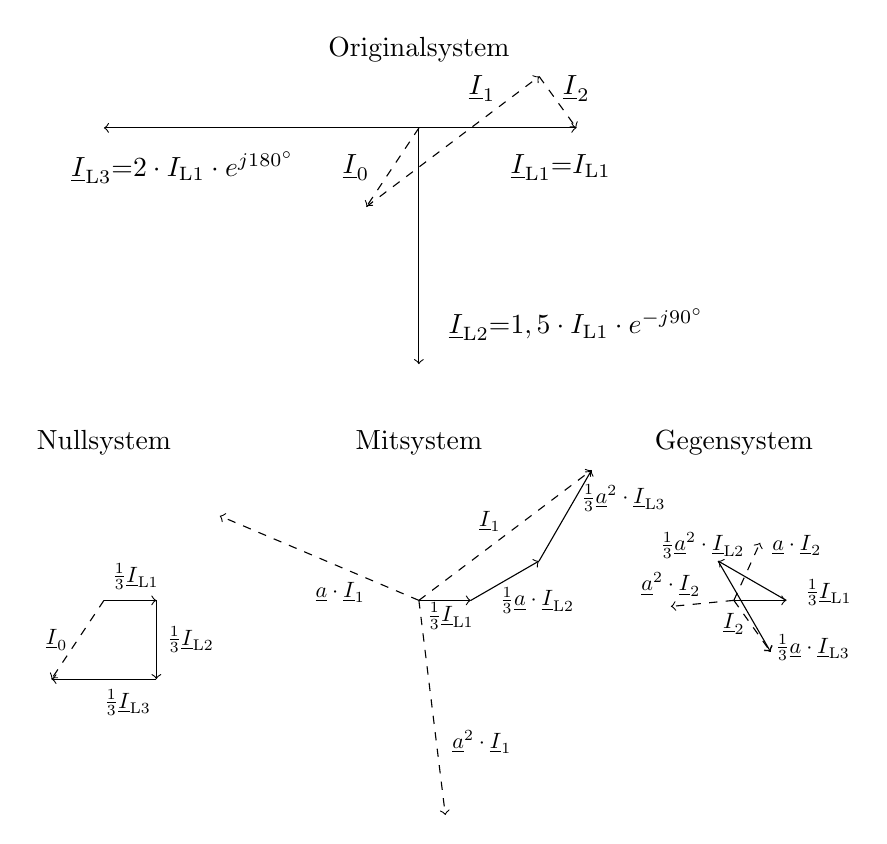
\begin{tikzpicture}
    \draw [->] (0, 0) -- (2, 0);
    \draw [->] (0, 0) -- (-4, 0);
    \draw [->] (0, 0) -- (0, -3);
    \draw [->] [dashed] (0, 0) -- (-0.666, -1);
    \draw [->] [dashed] (-0.666, -1) -- (1.527, 0.654);
    \draw [->] [dashed] (1.527, 0.654) -- (2, 0);

    \draw (1.8, -0.5) node {$\underline{I}_{\mathrm{L1}}{=}I_\mathrm{L1}$};
    \draw (-3, -0.5) node {$\underline{I}_{\mathrm{L3}}{=}2\cdot I_\mathrm{L1}\cdot e^{j180^{\circ}}$};
    \draw (2, -2.5) node {$\underline{I}_{\mathrm{L2}}{=}1,5\cdot I_\mathrm{L1}\cdot e^{-j90^{\circ}}$};
    \draw (0.8, 0.5) node {$\underline{I}_{\mathrm{1}}$};
    \draw (2, 0.5) node {$\underline{I}_{\mathrm{2}}$};
    \draw (-0.8, -0.5) node {$\underline{I}_{\mathrm{0}}$};

    \draw [->] [dashed] (0, -6) -- (2.193, -4.346);
    \draw [->] [dashed] (0, -6) -- (-2.529, -4.927);
    \draw [->] [dashed] (0, -6) -- (0.336, -8.726);
    \draw [->] (0, -6) -- (0.66, -6);
    \draw [->] (0.66, -6) -- (1.526, -5.5);
    \draw [->] (1.526, -5.5) -- (2.193, -4.346);

    \draw (0.9, -5) node [scale=0.8] {$\underline{I}_{\mathrm{1}}$};
    \draw (-1, -5.9) node [scale=0.8] {$\underline{a}\cdot\underline{I}_{\mathrm{1}}$};
    \draw (0.8, -7.8) node [scale=0.8] {$\underline{a}^2\cdot\underline{I}_{\mathrm{1}}$};
    \draw (0.4, -6.2) node [scale=0.8] {$\frac{1}{3}\underline{I}_{\mathrm{L1}}$};
    \draw (2.6, -4.7) node [scale=0.8] {$\frac{1}{3}\underline{a}^2\cdot\underline{I}_{\mathrm{L3}}$};
    \draw (1.5, -6) node [scale=0.8] {$\frac{1}{3}\underline{a}\cdot\underline{I}_{\mathrm{L2}}$};

    \draw [->] [dashed] (4, -6) -- (4.333, -5.268);
    \draw [->] [dashed] (4, -6) -- (4.467, -6.654);
    \draw [->] [dashed] (4, -6) -- (3.2, -6.077);
    \draw [->] (4, -6) -- (4.666, -6);
    \draw [->] (4.666, -6) -- (3.8, -5.5);
    \draw [->] (3.8, -5.5) -- (4.467, -6.654);

    \draw (4, -6.3) node [scale=0.8] {$\underline{I}_{\mathrm{2}}$};
    \draw (4.8, -5.3) node [scale=0.8] {$\underline{a}\cdot\underline{I}_{\mathrm{2}}$};
    \draw (3.2, -5.8) node [scale=0.8] {$\underline{a}^2\cdot\underline{I}_{\mathrm{2}}$};
    \draw (5.2, -5.9) node [scale=0.8] {$\frac{1}{3}\underline{I}_{\mathrm{L1}}$};
    \draw (3.6, -5.3) node [scale=0.8] {$\frac{1}{3}\underline{a}^2\cdot\underline{I}_{\mathrm{L2}}$};
    \draw (5, -6.6) node [scale=0.8] {$\frac{1}{3}\underline{a}\cdot\underline{I}_{\mathrm{L3}}$};

    \draw [->] [dashed] (-4, -6) -- (-4.666, -7);
    \draw [->] (-4, -6) -- (-3.334, -6);
    \draw [->] (-3.334, -6) -- (-3.334, -7);
    \draw [->] (-3.334, -7) -- (-4.666, -7);

    \draw (-4.6, -6.5) node [scale=0.8] {$\underline{I}_{\mathrm{0}}$};
    \draw (-3.6, -5.7) node [scale=0.8] {$\frac{1}{3}\underline{I}_{\mathrm{L1}}$};
    \draw (-2.9, -6.5) node [scale=0.8] {$\frac{1}{3}\underline{I}_{\mathrm{L2}}$};
    \draw (-3.7, -7.3) node [scale=0.8] {$\frac{1}{3}\underline{I}_{\mathrm{L3}}$};


    \draw (0, 1) node {Originalsystem};
    \draw (-4, -4) node {Nullsystem};
    \draw (0, -4) node {Mitsystem};
    \draw (4, -4) node {Gegensystem};

\end{tikzpicture}%
    }
    }{{\bf Zeigerdiagramme eines unsymmetrischen Systems.} Transformationen aus einem Originalsystem in Mit-, Gegen- und 
    Nullsystem. \label{ZeigerUnsym}}

\end{frame}

    \begin{frame}
        \ftx{Grundlagen - Matrixschreibweise}
    \s{
        Abb. \ref{ZeigerUnsym} zeigt das Zeigerdiagramm einer unsymmetrischen Belastung.
        Im Originalsystem ist an den Zeigern zu erkennen, dass sowohl die Winkel, wie auch die Amplituden vom symmetrischen Zustand abweichen.
        Durch die Transformation in die drei Systeme erhält man wiederum symmetrische Zeiger, mit denen dann einfacher gerechnet werden kann.
        An den Drehoperatoren und dem Vorfaktor von $\frac{1}{3}$ ist mit den Zeigern gut zu erkennen, wie sich die transformierten Ströme verhalten.
            
        Um die Transformationsgleichungen nicht immer vollständig hinschreiben zu müssen, können die Gleichungen auch in Matrixschreibweise geschrieben werden:

    \begin{eqa}
        \begin{bmatrix}
            \underline{I}_0 \\
            \underline{I}_1 \\
            \underline{I}_2 
        \end{bmatrix}
        = \frac{1}{3} \cdot
        \begin{bmatrix}
            1 & 1 & 1 \\
            1 & \underline{a} & \underline{a}^2 \\
            1 & \underline{a}^2 & \underline{a} 
        \end{bmatrix}
        \cdot
        \begin{bmatrix}
            \underline{I}_{\mathrm{L1}} \\
            \underline{I}_{\mathrm{L2}} \\
            \underline{I}_{\mathrm{L3}}
        \end{bmatrix}       \label{TraFoMatrix}
    \end{eqa}
 
    Die Schreibweise kann noch weiter vereinfacht werden, wenn der Term mit den Drehoperatoren und der Term mit Vorfaktor in einer Matrix zusammengfasst wird.
    Diese Matrix wird auch Symmetrierungsmatrix genannt:

    \begin{eqa} 
        \begin{bmatrix}
            \underline{T}
        \end{bmatrix}
        =\frac{1}{3} \cdot
        \begin{bmatrix}
            1 & 1 & 1 \\
            1 & \underline{a} & \underline{a}^2 \\
            1 & \underline{a}^2 & \underline{a} 
        \end{bmatrix}
        \end{eqa}

    In der Kompaktschreibweise erhält man so folgende Form:

    \begin{eqa}
        \begin{bmatrix}
            \underline{I}_{012}    
        \end{bmatrix}
        =
        \begin{bmatrix}
            \underline{T}    
        \end{bmatrix}
        \cdot
        \begin{bmatrix}
            \underline{I}_{\mathrm{L1L2L3}}    
        \end{bmatrix}
    \end{eqa}

    Gemäß den Rechenregeln für Matrizen kann mit der Inversen von $\begin{bmatrix}\underline{T}\end{bmatrix}$ die Rücktransformation erfolgen:

    \begin{eqa}
        \begin{bmatrix}
            \underline{I}_{\mathrm{L1}} \\
            \underline{I}_{\mathrm{L2}} \\
            \underline{I}_{\mathrm{L3}}
        \end{bmatrix}
        = \frac{1}{3} \cdot
        \begin{bmatrix}
            1 & 1 & 1 \\
            1 & \underline{a}^2 & \underline{a} \\
            1 & \underline{a} & \underline{a}^2 
        \end{bmatrix}
        \cdot
        \begin{bmatrix}
            \underline{I}_0 \\
            \underline{I}_1\\
            \underline{I}_2
        \end{bmatrix}
    \end{eqa}

    \begin{eqa}
        \begin{bmatrix}
            \underline{I}_{\mathrm{L1L2L3}}    
        \end{bmatrix}
        =
        \begin{bmatrix}
            \underline{T}    
        \end{bmatrix}^{-1}
        \cdot
        \begin{bmatrix}
            \underline{I}_{012}    
        \end{bmatrix}
    \end{eqa}

    }

    \b{
        \begin{itemize}
            \item Für eine vereinfachte Schreibweise können die Transformationsgleichungen in Matrixschreibweise beschrieben werden:
        \end{itemize}
        \begin{eqa}
            \begin{bmatrix}
                \underline{I}_0 \\
                \underline{I}_1 \\
                \underline{I}_2 
            \end{bmatrix}
            = \frac{1}{3} \cdot
            \begin{bmatrix}
                1 & 1 & 1 \\
                1 & \underline{a} & \underline{a}^2 \\
                1 & \underline{a}^2 & \underline{a} 
            \end{bmatrix}
            \cdot
            \begin{bmatrix}
                \underline{I}_{\mathrm{L1}} \\
                \underline{I}_{\mathrm{L2}} \\
                \underline{I}_{\mathrm{L3}}
            \end{bmatrix}       %\label{TraFoMatrix}
        \end{eqa}
        \begin{itemize}
            \item Die Schreibweise kann noch weiter vereinfacht werden, wenn der Term mit den Drehoperatoren und der Term mit Vorfaktor in einer Matrix zusammengfasst wird:
        \end{itemize}
        \begin{eqa} 
            \begin{bmatrix}
                \underline{T}
            \end{bmatrix}
            =\frac{1}{3} \cdot
            \begin{bmatrix}
                1 & 1 & 1 \\
                1 & \underline{a} & \underline{a}^2 \\
                1 & \underline{a}^2 & \underline{a} 
            \end{bmatrix}
            \end{eqa}
    }
\end{frame}

\begin{frame}
    \ftx{Grundlagen - Matrixschreibweise}
    \b{
    \begin{itemize}
        \item Werden die Gleichungen zusammengesetzt erhalt man in der Kompaktschreibweise folgende Gleichung:
    \end{itemize}
    \begin{eqa}
        \begin{bmatrix}
            \underline{I}_{012}    
        \end{bmatrix}
        =
        \begin{bmatrix}
            \underline{T}    
        \end{bmatrix}
        \cdot
        \begin{bmatrix}
            \underline{I}_{\mathrm{L1L2L3}}    
        \end{bmatrix}
    \end{eqa}
    \begin{itemize}
        \item Gemäß den Rechenregeln für Matrizen kann mit der Inversen von $\begin{bmatrix}\underline{T}\end{bmatrix}$ die Rücktransformation erfolgen:
    \end{itemize}
    \begin{eqa}
        \begin{bmatrix}
            \underline{I}_{\mathrm{L1}} \\
            \underline{I}_{\mathrm{L2}} \\
            \underline{I}_{\mathrm{L3}}
        \end{bmatrix}
        = \frac{1}{3} \cdot
        \begin{bmatrix}
            1 & 1 & 1 \\
            1 & \underline{a}^2 & \underline{a} \\
            1 & \underline{a} & \underline{a}^2 
        \end{bmatrix}
        \cdot
        \begin{bmatrix}
            \underline{I}_0 \\
            \underline{I}_1\\
            \underline{I}_2
        \end{bmatrix}
    \end{eqa}
    \begin{eqa}
        \begin{bmatrix}
            \underline{I}_{\mathrm{L1L2L3}}    
        \end{bmatrix}
        =
        \begin{bmatrix}
            \underline{T}    
        \end{bmatrix}^{-1}
        \cdot
        \begin{bmatrix}
            \underline{I}_{012}    
        \end{bmatrix}
    \end{eqa}
    }
\end{frame}


\begin{frame}
    \ftx{Systemarten}

    \begin{Merksatz}{Mit-, Gegen- und Nullsystem}
        Ein System wird zur Analyse in die drei Systeme: Mitsystem, Gegensystem und Nullsystem transformiert. \\
        Das {\bf Mitsystem} wird mit dem Index 1 versehen: \qquad  $\underline{I}_1$ \\
        Das {\bf Gegensystemsystem} wird mit dem Index 2 versehen: \qquad $\underline{I}_2$ \\
        Das {\bf Nullsystem} wird mit dem Index 0 versehen: \qquad $\underline{I}_0$ 
    \end{Merksatz}
\end{frame}



\begin{frame}
    \ftb{Drehstromleistung}

\s{
    Wie die Leistung berechnet wird, wurde bereits im Kapitel Drehstrom erläutert.
    Auch hier kann die Gleichung zur Leistungsberechnung zur Vereinfachung in Matrizenschreibweise ausgedrückt werden:
}
\b{
    \begin{itemize}
        \item Die Gleichung zur Leistungsberechnung kann zur Vereinfachung auch in Matrizenschreibweise ausgedrückt werden
    \end{itemize}
}
    \begin{eqa}
        \underline{S}_{\mathrm{L1L2L3}}&=\underline{U}_{\mathrm{L1}}\cdot\underline{I}_{\mathrm{L1}}^*+\underline{U}_{\mathrm{L2}}\cdot\underline{I}_{\mathrm{L2}}^*+\underline{U}_{\mathrm{L3}}\cdot\underline{I}_{\mathrm{L3}}^* \\
        &=
        \begin{bmatrix}
            \underline{U}_{\mathrm{L1}} & \underline{U}_{\mathrm{L2}} & \underline{U}_{\mathrm{L3}}
        \end{bmatrix}
        \cdot
        \begin{bmatrix}
            \underline{I}_{\mathrm{L1}}^* \\
            \underline{I}_{\mathrm{L2}}^* \\
            \underline{I}_{\mathrm{L3}}^*
        \end{bmatrix}
        =
        \begin{bmatrix}
            \underline{U}_{\mathrm{L1L2L3}}
        \end{bmatrix}
        \cdot
        \begin{bmatrix}
            \underline{I}_{\mathrm{L1L2L3}}
        \end{bmatrix}_t
        ^*      \notag
    \end{eqa}

\end{frame}
\begin{frame}
    \ftx{Drehstromleistung und Komponentenleistung}
    

\s{
    Mit den gegebenen Drehoperatoren können die Ströme und Spannungen in einem symmetrische System auf jeweils eine Phase bezogen werden 
    ($\underline{U}_{\mathrm{L2}}=\underline{a}^2\cdot\underline{U}_{\mathrm{L1}}, \underline{U}_{\mathrm{L3}}=\underline{a}\cdot\underline{U}_{\mathrm{L1}}$)

    Daraus ergibt sich für die Leistung die bekannte Vereinfachung:
}
\b{
    \begin{itemize}
        \item Mit den Drehoperatoren können die Spannungen und Ströme auf eine Phase bezogen werden
        \item Draus ergibt sich die bekannte Vereinfachung:
    \end{itemize}
}
    \begin{eqa}
        \underline{S}_{\mathrm{L1L2L3}}&=\underline{U}_{\mathrm{L1}}\cdot\underline{I}_{\mathrm{L1}}^*+\underline{U}_{\mathrm{L1}}\cdot\underline{I}_{\mathrm{L1}}^*+\underline{U}_{\mathrm{L1}}\cdot\underline{I}_{\mathrm{L1}}^* \\
        &=3\cdot\underline{U}_{\mathrm{L1}}\cdot\underline{I}_{\mathrm{L1}}^*
    \end{eqa}
\end{frame}

\begin{frame}
    \ftx{Drehstromleistung und Komponentenleistung}

\s{
    Nun kann mit der Matrixschreibweise die Transformation in die neuen Systeme berechnet werden:
}
\b{
    \begin{itemize}
        \item Nun kann mit der Matrixschreibweise die Transformation in die neuen Systeme berechnet werden:
    \end{itemize}
}
    \begin{eqa}
        \begin{bmatrix}
            \underline{U}_{\mathrm{L1L2L3}}
        \end{bmatrix}
        &=
        (
            \begin{bmatrix}
                \underline{T}
            \end{bmatrix}^{-1}
            \cdot
            \begin{bmatrix}
                \underline{U}_{012}
            \end{bmatrix}
        )
        =
        \begin{bmatrix}
            \underline{U}_{012}
        \end{bmatrix}
        \cdot
        \begin{bmatrix}
            \underline{T}
        \end{bmatrix}^{-1} \\
        \begin{bmatrix}
            \underline{I}_{\mathrm{L1L2L3}}
        \end{bmatrix}^*
        &=
        (
            \begin{bmatrix}
                \underline{T}
            \end{bmatrix}^{-1}
            \cdot
            \begin{bmatrix}
                \underline{I}_{012}
            \end{bmatrix}
        )^*
        =
        \begin{bmatrix}
            \underline{T}
        \end{bmatrix}^{-1*}
        \cdot
        \begin{bmatrix}
            \underline{I}_{012}
        \end{bmatrix}^*   \\         
        \underline{S}_{\mathrm{L1L2L3}}
        &=
        \begin{bmatrix}
            \underline{U}_{012}
        \end{bmatrix}_t
        \cdot
        \begin{bmatrix}
            \underline{T}
        \end{bmatrix}^{-1}
        \cdot
        \begin{bmatrix}
            \underline{T}
        \end{bmatrix}^{-1*}
        \cdot
        \begin{bmatrix}
            \underline{I}_{012}
        \end{bmatrix}^* \\
        &=
        \begin{bmatrix}
            \underline{U}_{012}
        \end{bmatrix}_t
        \cdot
        \begin{bmatrix}
            1 & 1 & 1 & \\
            1 & \underline{a}^2 & \underline{a} \\
            1 & \underline{a} & \underline{a}^2
        \end{bmatrix}
        \cdot
        \begin{bmatrix}
            1 & 1 & 1 & \\
            1 & \underline{a}^2 & \underline{a} \\
            1 & \underline{a} & \underline{a}^2
        \end{bmatrix}^*
        \cdot
        \begin{bmatrix}
            \underline{I}_{012}
        \end{bmatrix}^* \notag\\
        &=
        \begin{bmatrix}
            \underline{U}_{012}
        \end{bmatrix}_t
        \cdot
        \begin{bmatrix}
            1 & 1 & 1 & \\
            1 & \underline{a}^2 & \underline{a} \\
            1 & \underline{a} & \underline{a}^2
        \end{bmatrix}
        \cdot
        \begin{bmatrix}
            1 & 1 & 1 & \\
            1 & \underline{a} & \underline{a}^2 \\
            1 & \underline{a}^2 & \underline{a}
        \end{bmatrix}
        \cdot
        \begin{bmatrix}
            \underline{I}_{012}
        \end{bmatrix}^* \notag\\
        &=
        \begin{bmatrix}
            \underline{U}_{012}
        \end{bmatrix}
        \cdot
        \begin{bmatrix}
            3 & 0 & 0 \\
            0 & 3 & 0 \\
            0 & 0 & 3
        \end{bmatrix}
        \cdot
        \begin{bmatrix}
            \underline{I}_{012}
        \end{bmatrix}^* \notag\\
        &=3\cdot(\underline{U}_0\cdot\underline{I}_o^*+\underline{U}_1\cdot\underline{I}_1^*+\underline{U}_2\cdot\underline{I}_2^*)=3\cdot\underline{S}_{012} \notag
    \end{eqa}

\end{frame}

\begin{frame}
    \ftb{Ersatzschaltbilder}
\s{
    ESB dienen grundlegend immmer der einfacheren Betrachtung und einem erleichterten Verständniss der Komponenten.
    Es sollen sich nun verschiedene Betriebsmittel angeschaut werden und wie sich die Transformationen in verschiedenen Netzsituationen verhalten.
}
\b{
    \begin{itemize}
        \item ESB dienen grundlegend immmer der einfacheren Betrachtung und einem erleichterten Verständniss der Komponenten
        \item Es sollen sich nun verschiedene Betriebsmittel angeschaut werden und wie sich die Transformationen in verschiedenen Netzsituationen verhalten
    \end{itemize}
}
\end{frame}

\begin{frame}
        \ftc{Symmetrische Spannungsquelle}
\s{
    Symmetrische Spannungsquellen findet man z.B. bei der Netzeinspeisung und auch bei Synchronmaschienen.
    Im ersten Schritt wird sich das Ausgangssystems angeschaut.
    Die Zusammenhänge zwischen der Sternspannung und den einzelnen Phasen ist bereits aus dem Kapitel ??? bekannt.
    Mit der Formel für die Transformation (vgl. \ref{TraFoMatrix}) lässt sich nun rechnerisch zeigen, dass in einem solchen symmetrischen Fall die Spannungen des Gegen- und Nullsystems 0 ergeben.

    Lediglich im Mitsystem tritt eine treibende Spannung, in Höhe der Sternspannung auf:
}
\b{
    \begin{itemize}
        \item Als erste Komponente werden die Spannungsquellen betrachtet
        \item Die Zusammenhänge zwischen der Sternspannung und den einzelnen Phasen sind bereits bekannt
        \item Es wird die Formel für die Transformation herangezogen und in die Matrixschreibweise überführt
    \end{itemize}
}
    \begin{eqa}
        \begin{bmatrix}
            \underline{U}_0 \\
            \underline{U}_1 \\
            \underline{U}_2
        \end{bmatrix}
        &=
        \frac{1}{3}\cdot
        \begin{bmatrix}
            1 & 1 & 1 & \\
            1 & \underline{a} & \underline{a}^2 \\
            1 & \underline{a}^2 & \underline{a}
        \end{bmatrix}
        \cdot
        \begin{bmatrix}
            \underline{U}_{\mathrm{L1}} \\
            \underline{U}_{\mathrm{L2}} \\
            \underline{U}_{\mathrm{L3}}
        \end{bmatrix} \\
        \begin{bmatrix}
            \underline{U}_{012}
        \end{bmatrix}
        &=
        \begin{bmatrix}
            \underline{T}
        \end{bmatrix}
        \cdot
        \begin{bmatrix}
            \underline{U}_{\Stern} \\
            \underline{a}^2\cdot\underline{U}_{\Stern} \\
            \underline{a}\cdot\underline{U}_{\Stern}
        \end{bmatrix}
    \end{eqa}

\end{frame}
    \begin{frame}
        \ftx{Symmetrische Spannungsquelle}
        
  \s{
    Löst man die Gleichungen für die transformierten Systeme auf erhält man die Spannungsergebnisse:
  }
  \b{
    \begin{itemize}
        \item Wird die Gleichung für die transformierten Systeme aufgelöst, erhält man die Spannungsergebnisse
    \end{itemize}
  }
    \begin{eqa}
        \underline{U}_0&=\frac{1}{3}\cdot{U}_{\Stern}\cdot(1+\underline{a}^2+\underline{a})=0 \\
        \underline{U}_1&=\frac{1}{3}\cdot{U}_{\Stern}\cdot(1+\underline{a}\cdot\underline{a}^2+\underline{a}^2\cdot\underline{a})=U_{\Stern} \\
        \underline{U}_2&=\frac{1}{3}\cdot{U}_{\Stern}\cdot(1+\underline{a}^2\cdot\underline{a}^2+\underline{a}\cdot\underline{a})=0 
    \end{eqa}

\end{frame}
    \begin{frame}
        \ftx{Symmetrische Spannungsquelle}
  \s{
    Mit den Ergebnissen des Gegen- und Nullsystems kann bildlich gesagt werden, dass diese kurzgeschlossen sind.
    So können für die drei transformierten Systeme die jeweiligen ESB erstellt werden:
  }
  \b{
    \begin{itemize}
        \item Den Spannung entsprechend können die ESB der einzelnen Systeme aufgestellt werden
        \item Mit den Ergebnissen des Gegen- und Nullsystems kann bildlich gesagt werden, dass diese kurzgeschlossen sind
    \end{itemize}
  }
    \fu{
        \begin{circuitikz}
    \draw (4, 0) to[short, o-] (0, 0)
    to [short] (0, 1.2)
    to[short, -o] (4, 1.2);

    \draw (4, 1.4) to[short, o-] (0, 1.4)
    to [short] (0, 2.6)
    to[short, -o] (4, 2.6);

    \draw (4, 2.8) to[short, o-] (0, 2.8)
    to [sV, v<=$U_{\Stern}$] (0, 4)
    to[short, -o] (4, 4);

    \draw (2, 0.6) node {Nullsystem};
    \draw [->](4, 1) -- (4, 0.2);
    \draw (4.4, 0.6) node {$\underline{U}_0$};

    \draw (2, 2) node {Gegensystem};
    \draw [->](4, 2.4) -- (4, 1.6);
    \draw (4.4, 2) node {$\underline{U}_2$};

    \draw (2, 3.4) node {Mitsystem};
    \draw [->](4, 3.8) -- (4, 3);
    \draw (4.4, 3.4) node {$\underline{U}_1$};

\end{circuitikz}
    }{{\bf Ersatzschaltbilder der transformierten Spannungsquelle.} Bei der symmetrischen Spannungsquelle verfügt nur das ESB 
    des Mitsystems über die Spannungsquelle. \label{ESBSymQuellen}}

    \s{
        In der Abbildung \ref{ESBSymQuellen} soll nochmal deutlich hervorgehoben werden, dass einerseits drei einzelne System 
        gebildet werden und weiter, dass in dem spezial Fall der symmetrischen Quellen nur in einem der Systeme eine Spannung 
        auftaucht.
    }
    
\end{frame}

\begin{frame}
    \ftc{Symmetrische Last}
\s{
    Für die Betrachtung der Lasten soll eine Sternschaltung mit Rückleiter gewählt werden. 
    Es wird in jedem Leiter, auch im Rückleiter, eine Impedanz Z angenommen.
    Für den symmetrischen Fall werden die Impedanzen als gleich groß angenommen, lediglich die Impedanz im Rückleiter kann von den anderen abweichen und bekommt einen eigenen Index.

    Für das Originalsystem werden die Gleichung für die Spannung folgendermaßen aufgestellt:
}
\b{
    \begin{itemize}
        \item Für die Betrachtung der Lasten soll eine Sternschaltung mit Rückleiter gewählt werden
        \item Es wird in jedem Leiter, auch im Rückleiter, eine Impedanz Z angenommen
        \item Für den symmetrischen Fall werden die Impedanzen als gleich groß angenommen, lediglich die Impedanz im Rückleiter kann von den anderen abweichen und bekommt einen eigenen Index.
    \end{itemize}
}

    \begin{eqa}
        \underline{U}_{\mathrm{L1}}=\underline{Z}\cdot\underline{I}_{\mathrm{L1}}+\underline{Z}_\mathrm{E}\cdot(\underline{I}_{\mathrm{L1}}+\underline{I}_{\mathrm{L2}}+\underline{I}_{\mathrm{L3}}) \\
        \underline{U}_{\mathrm{L2}}=\underline{Z}\cdot\underline{I}_{\mathrm{L2}}+\underline{Z}_\mathrm{E}\cdot(\underline{I}_{\mathrm{L1}}+\underline{I}_{\mathrm{L2}}+\underline{I}_{\mathrm{L3}}) \\
        \underline{U}_{\mathrm{L3}}=\underline{Z}\cdot\underline{I}_{\mathrm{L3}}+\underline{Z}_\mathrm{E}\cdot(\underline{I}_{\mathrm{L1}}+\underline{I}_{\mathrm{L2}}+\underline{I}_{\mathrm{L3}})
    \end{eqa}

\end{frame}
    \begin{frame}
        \ftx{Symmetrische Last}
    \s{
    Auch hier kann mittels Matrixschreibweise vereinfacht werden:
    }
    \b{
        \begin{itemize}
            \item Auch hier kann mittels Matrixschreibweise vereinfacht werden
        \end{itemize}
    }
    \begin{eqa}
        \begin{bmatrix}
            \underline{U}_{\mathrm{L1}} \\
            \underline{U}_{\mathrm{L2}} \\
            \underline{U}_{\mathrm{L3}}
        \end{bmatrix}
        =
        \begin{bmatrix}
            \underline{Z}+\underline{Z}_\mathrm{E} & \underline{Z}_\mathrm{E} & \underline{Z}_\mathrm{E} \\
            \underline{Z}_\mathrm{E} & \underline{Z}+\underline{Z}_\mathrm{E} & \underline{Z}_\mathrm{E} \\
            \underline{Z}_\mathrm{E} & \underline{Z}_\mathrm{E} & \underline{Z}+\underline{Z}_\mathrm{E}
        \end{bmatrix}
        \cdot
        \begin{bmatrix}
            \underline{I}_{\mathrm{L1}} \\
            \underline{I}_{\mathrm{L2}} \\
            \underline{I}_{\mathrm{L3}}
        \end{bmatrix}
    \end{eqa}

    Mit...
    
    \begin{eqa}
        \begin{bmatrix}
            \underline{Z}_{\mathrm{L1L2L3}}
        \end{bmatrix}
        =
        \begin{bmatrix}
            \underline{Z}+\underline{Z}_\mathrm{E} & \underline{Z}_\mathrm{E} & \underline{Z}_\mathrm{E} \\
            \underline{Z}_\mathrm{E} & \underline{Z}+\underline{Z}_\mathrm{E} & \underline{Z}_\mathrm{E} \\
            \underline{Z}_\mathrm{E} & \underline{Z}_\mathrm{E} & \underline{Z}+\underline{Z}_\mathrm{E}
        \end{bmatrix}
      \end{eqa}

      ...ergibt sich

      \begin{eqa}
        \begin{bmatrix}
            \underline{U}_{\mathrm{L1L2L3}}
        \end{bmatrix}
        =
        \begin{bmatrix}
            \underline{Z}_{\mathrm{L1L2L3}}
        \end{bmatrix}
        \cdot
        \begin{bmatrix}
            \underline{I}_{\mathrm{L1L2L3}}
        \end{bmatrix}
      \end{eqa}

    \end{frame}
      \begin{frame}
        \ftx{Symmetrische Last}
      \s{
      Wird mit den Transformationsgleichungen umgeformt folgt:
      }
      \b{
        \begin{itemize}
            \item Wird mit den Transformationsgleichungen umgeformt folgt:
        \end{itemize}
      }
    \begin{eqa}
    \begin{bmatrix}
        \underline{T}
    \end{bmatrix}^{-1}
    \cdot
    \begin{bmatrix}
        \underline{U}_{012}
    \end{bmatrix}
    =
    \begin{bmatrix}
        \underline{Z}_{\mathrm{L1L2L3}}
    \end{bmatrix}
    \begin{bmatrix}
        \underline{T}
    \end{bmatrix}^{-1}
    \cdot
    \begin{bmatrix}
        \underline{I}_{012}
    \end{bmatrix}
    \end{eqa}

    \s{
    Bei den symmetrischen Spannungsquellen konnte aus der Transformation die Spannung abhängig vom Originalsystem errechnet werden.
    Das gleiche soll auf für die Impedanzen für die Verbraucher geschafft werden.
    Dafür müssen die aufgestellten Gleichunge noch so umgeformt werden, dass sich ein Verhältnis von transformierten Impedanzen und Impedanzen des Originalsystem ergibt.
    Um das zu erreichen werden beide Seiten erst mit $\begin{bmatrix}\underline{T}\end{bmatrix}$ erweitert und dann auf Grundlage des Ohmschen-Gesetzes umgestellt.
    }
    \b{
        \begin{itemize}
            \item Wie bei den Spannungsquellen soll aus der Transformation die Spannung abhängig vom Originalsystem errechnet werden
            \item Durch Umstellung wird ein Verhältnis zwischen transformierten Impedanzen und Impedanzen des Originalsystems geschaffen
        \end{itemize}
    }
    \begin{eqa}
        \begin{bmatrix}
            \underline{T}
        \end{bmatrix}
        \cdot
        \begin{bmatrix}
            \underline{T}
        \end{bmatrix}^{-1}
        \cdot
        \begin{bmatrix}
            \underline{U}_{012}
        \end{bmatrix}
        &=
        \begin{bmatrix}
            \underline{T}
        \end{bmatrix}
        \cdot
        \begin{bmatrix}
            \underline{Z}_{\mathrm{L1L2L3}}
        \end{bmatrix}
        \begin{bmatrix}
            \underline{T}
        \end{bmatrix}^{-1}
        \cdot
        \begin{bmatrix}
            \underline{I}_{012}
        \end{bmatrix}   \\
        \begin{bmatrix}
            \underline{U}_{012}
        \end{bmatrix}
        &=
        \begin{bmatrix}
            \underline{T}
        \end{bmatrix}
        \cdot
        \begin{bmatrix}
            \underline{Z}_{\mathrm{L1L2L3}}
        \end{bmatrix}
        \begin{bmatrix}
            \underline{T}
        \end{bmatrix}^{-1}
        \cdot
        \begin{bmatrix}
            \underline{I}_{012}
        \end{bmatrix}   \\
        \begin{bmatrix}
            \underline{Z}_{012}
        \end{bmatrix}
        &=
        \begin{bmatrix}
            \underline{T}
        \end{bmatrix}
        \cdot
        \begin{bmatrix}
            \underline{Z}_{\mathrm{L1L2L3}}
        \end{bmatrix}
        \begin{bmatrix}
            \underline{T}
        \end{bmatrix}^{-1}
      \end{eqa}

    \end{frame}

      \begin{frame}
        \ftx{Symmetrische Last}
   
    \s{
    Wird die Matrixoperation der letzten Gleichung durchgeführt, dann ergibt sich der gewünschte Zusammenhanhg von Original- und Transformationssystem.
    }
    \b{
        \begin{itemize}
            \item Mit der Druchführung der Matrixoperation ergibt sich der gewünschte Zusammenhang von Original- und Transformationssystem
        \end{itemize}
    }
    \begin{eqa}
        \begin{bmatrix}
            \underline{Z}_{012}
        \end{bmatrix}
        =
        \begin{bmatrix}
                \underline{Z}+3\underline{Z}_E & 0 & 0 \\
                0 & \underline{Z} & 0 \\
                0 & 0 & \underline{Z}
        \end{bmatrix}
    \end{eqa}

\end{frame}
    \begin{frame}
        \ftx{Symmetrische Last}
   
    \s{
    Nun können auch für die symmetrischen Lasten die jeweiligen ESB der transformierten Systeme aufgestellt werden:
    }
    \b{
        \begin{itemize}
            \item Mit dem errechneten Zusammenhängen können die ESB der einzelnen Systeme aufgestellt werden
            \item Im Mit- und Gegensystem treten die gleichen Impedanzen auf
            \item Im Nullsystem tritt zudem eine Impedanz mit dreifachem Wert auf
        \end{itemize}
    }
    \fu{
       \begin{circuitikz}
    \draw (0, 0) to[R, l_=$3\cdot\underline{Z}_{\mathrm{E}}$, o-] (4, 0)
    to [short] (4, 1.2)
    to[R=$\underline{Z}$, -o] (0, 1.2);

    \draw (0, 1.6) to[short, o-] (4, 1.6)
    to [short] (4, 2.8)
    to[R=$\underline{Z}$, -o] (0, 2.8);

    \draw (0, 3.2) to[short, o-] (4, 3.2)
    to [short] (4, 4.4)
    to[R=$\underline{Z}$, -o] (0, 4.4);

    \draw [->](0, 1) -- (0, 0.2);
    \draw (-0.4, 0.6) node {$\underline{U}_0$};

    \draw [->](0, 2.6) -- (0, 1.8);
    \draw (-0.4, 2.2) node {$\underline{U}_2$};

    \draw [->](0, 4.2) -- (0, 3.4);
    \draw (-0.4, 3.8) node {$\underline{U}_1$};

\end{circuitikz}
    }{{\bf Ersatzschaltbilder der transformierten Last.} Bei der symmetrischen Last weisen die drei Systeme alle eine 
    symmetrische Impedanz auf, jedoch verfügt das Nullsystem zusätzlich noch über die dreifache Impedanz für einen 
    Rückleiter. \label{ESBSymLasten}}

    \s{
    In Abb. \ref{ESBSymLasten} treten im Mit- und Gegensystem die gleichen Impedanzen auf.
    Sollten die Verbraucher im Dreieck verschaltet sein, müssten die Impedanzen mit den bekannten Verhältnissen in Sterngrößen umgerechnet werden.
    Für die Nullimpedanzen gilt, dass Ströme nur fließen, wenn auch in der Realität eine Verbindung zu einem Stern besteht.
    Dann treten die Impedanzen im Rückleiter mit dreifachem Wert auf.
    }
  
  
\end{frame}

\begin{frame}
    \ftc{Symmetrische Leitungen}

    \s{
    Die Leitung ist die Verbindung zwischen der Spannungsquelle und den Verbrauchern.
    Bisher wurden in den Betrachtungen zum Drehstrom nur unterschieden zwischen Erzeugung und Verbrauchern.
    Mit den Leitungen kommt nun eine zusätzliche Komponente hinzu, die separat betrachtet werden soll.
    Leitungen weisen grundsätzlich Eigenimpedanzen, Koppelimpedanzen und Leiter-Erde-Impedanzen auf. Die Leiter-Erde-Impedanzen können jedoch vernachlässigt werden.
    So hat jeder Leiter eine Eigenimpedanzen und zwei Koppelimpedanzen, also zu den jeweils anderen Leitern.
    Die Spannung für diese Berechnung wird definiert als Differenz der Spannungen am Anfang und am Ende der Leitung.
    So lässt sich die Matrix-Gleichung für ein Leitungssystem aufstellen:
    }

    \b{
        \begin{itemize}
            \item Die Leitung ist die Komponente, die die Spannungsquelle und die Verbraucher verbindet
            \item Es treten grundsätzlich Eigenimpedanzen und Koppelimpedanzen auf (Leiter-Erde-Impedanzen werden vernachlässigt)
            \item Dementsprechend treten in jedem Strang eine Eigenimpedanzen und zwei Koppelimpedanzen (zu den anderen Strängen) auf
            \item Die Spannung über einen Strang wird definiert als Spannungsdifferenz der Spannung am Anfang und am Ende der Leitung
        \end{itemize}
    }
    \begin{eqa}
        \begin{bmatrix}
            \underline{U}_{\mathrm{L1A}}-\underline{U}_{\mathrm{L1B}} \\
            \underline{U}_{\mathrm{L2A}}-\underline{U}_{\mathrm{L2B}} \\
            \underline{U}_{\mathrm{L3A}}-\underline{U}_{\mathrm{L3B}}
        \end{bmatrix}
        =
        \begin{bmatrix}
            \underline{Z}_\mathrm{S} & \underline{Z}_\mathrm{K} & \underline{Z}_\mathrm{K} \\
            \underline{Z}_\mathrm{K} & \underline{Z}_\mathrm{S} & \underline{Z}_\mathrm{K} \\
            \underline{Z}_\mathrm{K} & \underline{Z}_\mathrm{K} & \underline{Z}_\mathrm{S}
        \end{bmatrix}
        \cdot
        \begin{bmatrix}
            \underline{I}_{\mathrm{L1}} \\
            \underline{I}_{\mathrm{L2}} \\
            \underline{I}_{\mathrm{L3}}
        \end{bmatrix}
    \end{eqa}

\end{frame}
    \begin{frame}
        \ftx{Symmetrische Leitungen}
  
\s{
    Daraus kann wieder eine Kompaktschreibweise abgeleitet werden (Mit $U_{\mathrm{L1A}}-U_{\mathrm{L1B}}=U_{\mathrm{L1}}$, ...):
}
\b{
    \begin{itemize}
        \item Mit $U_{\mathrm{L1A}}-U_{\mathrm{L1B}}=U_{\mathrm{L1}}$, ... kann wieder eine Kompaktschreibweise abgeleitet werden
    \end{itemize}
}
    \begin{eqa}
        \begin{bmatrix}
            \underline{U}_{\mathrm{L1L2L3}}
        \end{bmatrix}
        =
        \begin{bmatrix}
            \underline{Z}_{\mathrm{L1L2L3}}
        \end{bmatrix}
        \cdot
        \begin{bmatrix}
            \underline{I}_{\mathrm{L1L2L3}}
        \end{bmatrix}
    \end{eqa}

    \s{
    Es liegt nun eine sehr ähnliche Gleichung vor, wie die bei den symmetrischen Verbrauchern.
    Auch hier soll die Gleichung so umgeformt werden, dass eine direkte Abhängigkeit von Originalsystem und Transformationssystem vorliegt.
    Da die Gleichung grundlegend gleich aufgebaut ist, können die gleichen Erweiterungen und Umformungen durchgeführt werden, wie bereits bei den symmetrischen Verbrauchern:
    }
    \b{
        \begin{itemize}
            \item Die Gleichung ist nun sehr ähnlich wie bei den symmetrischen Verbrauchern
            \item Somit können die gleichen Umformungen durchgeführt werden, sodass auch hier ine direkte Abhängigkeit von Originalsystem und Transformationssystem vorliegt
        \end{itemize}
    }
    \begin{eqa}
        \begin{bmatrix}
            \underline{Z}_{012}
        \end{bmatrix}
        =
        \begin{bmatrix}
            \underline{Z}_\mathrm{S}+2\cdot\underline{Z}_\mathrm{K} & 0 & 0 \\
            0 & \underline{Z}_\mathrm{S}-\underline{Z}_\mathrm{K} & 0 \\
            0 & 0 & \underline{Z}_\mathrm{S}-\underline{Z}_\mathrm{K}
        \end{bmatrix}
      \end{eqa}
\s{
    Wichtig ist bei der Umformung immer, dass die umgeformte Impedanzmatrix nur aus Werten auf der Hauptdiagonale besteht, damit es nur direkte Zusammenhänge zwischen den einzenlen Leitern und den Transformationssytemen gibt.
}

\end{frame}
\begin{frame}
    \ftx{Symmetrische Leitungen}
    

    \fu{
        \begin{circuitikz}
    \draw (0, 0) to[short, o-o] (7.5, 0) [dashed];

    \draw (0, 1.5) to[short, f=$\underline{I}_{\mathrm{L3}}$, o-] (1.5, 1.5)
    to[R=$\underline{Z}_{\mathrm{S}}$] (3, 1.5)
    to[short] (4.5, 1.5)
    to[R] (6, 1.5)
    to[R, -o] (7.5, 1.5);

    \draw (0, 3) to[short, f=$\underline{I}_{\mathrm{L2}}$, o-] (1.5, 3)
    to[R=$\underline{Z}_{\mathrm{S}}$] (3, 3)
    to[R] (4.5, 3)
    to[R] (6, 3)
    to[short, -o] (7.5, 3);


    \draw (0, 4.5) to[short, f=$\underline{I}_{\mathrm{L1}}$, o-] (1.5, 4.5)
    to[R=$\underline{Z}_{\mathrm{S}}$] (3, 4.5)
    to[R] (4.5, 4.5)
    to[short] (6, 4.5)
    to[R, -o] (7.5, 4.5);


    \draw [->](-1.8, 4.5) -- (-1.8, 0);
    \draw (-1.3, 3.7) node {$\underline{U}_{\mathrm{L1A}}$};
    \draw [->](-1.5, 3) -- (-1.5, 0);
    \draw (-1, 2.2) node {$\underline{U}_{\mathrm{L2A}}$};
    \draw [->](-1.2, 1.5) -- (-1.2, 0);
    \draw (-0.7, 0.7) node {$\underline{U}_{\mathrm{L3A}}$};

    \draw [->](9.3, 4.5) -- (9.3, 0);
    \draw (8.8, 3.7) node {$\underline{U}_{\mathrm{L1B}}$};
    \draw [->](9, 3) -- (9, 0);
    \draw (8.5, 2.2) node {$\underline{U}_{\mathrm{L2B}}$};
    \draw [->](8.7, 1.5) -- (8.7, 0);
    \draw (8.2, 0.7) node {$\underline{U}_{\mathrm{L3B}}$};


    \draw (-0.4, 0) node {$N_{\mathrm{Q}}$};
    \draw (7.9, 0) node {$N_{\mathrm{V}}$};

    \draw (-0.4, 1.5) node {$L_3$};
    \draw (-0.4, 3) node {$L_2$};
    \draw (-0.4, 4.5) node {$L_1$};
    \draw (7.9, 1.5) node {$L_3$};
    \draw (7.9, 3) node {$L_2$};
    \draw (7.9, 4.5) node {$L_1$};

    \draw [-] [dashed] (3.75, 4.5) -- (3.75, 3);
    \draw (3.75, 4.5) node[circ] {};
    \draw (3.75, 3) node[circ] {};
    \draw (4.1, 3.75) node {$\underline{Z}_{\mathrm{K}}$};

    \draw [-] [dashed] (5.24, 3) -- (5.25, 1.5);
    \draw (5.25, 3) node[circ] {};
    \draw (5.25, 1.5) node[circ] {};
    \draw (5.6, 2.25) node {$\underline{Z}_{\mathrm{K}}$};

    \draw [-] [dashed] (6.75, 4.5) -- (6.75, 1.5);
    \draw (6.75, 4.5) node[circ] {};
    \draw (6.75, 1.5) node[circ] {};
    \draw (7.1, 3.75) node {$\underline{Z}_{\mathrm{K}}$};

\end{circuitikz}
    }{{\bf Ersatzschaltbilder der transformierten Leitung.} ESB einer symmetrischen Leitung mit den drei Phasen $L_\mathrm{1}$,
    $L_\mathrm{2}$ und $L_\mathrm{3}$ sowie gestrichelt die angedeutete Leitung der Sternpunktbehandlung. \label{ESBSymLeitung}}

    \s{
    Abb. \ref{ESBSymLeitung} zeigt das ESB der drei Systeme für symmetrische Leitungen.
    Die gestrichelte Leitung soll die Sternpunktbehandlung auf Erzeugungs- und Verbraucherseite widerspiegeln zur Referenz der Sternspannungen.
    }
    \b{
    \begin{itemize}
        \item ESB der drei Systeme für symmetrische Leitungen
        \item Die gestrichelte Leitung soll die Sternpunktbehandlung auf Erzeugungs- und Verbraucherseite widerspiegeln zur Referenz der Sternspannungen
    \end{itemize}
}

\end{frame}




